\documentclass[11pt,oneside]{book}

% ========== 基础 ==========
\usepackage[a4paper,margin=2.5cm]{geometry}
\usepackage{fontspec}
\setmainfont{Times New Roman}
\usepackage{xeCJK}
\IfFontExistsTF{Microsoft YaHei}{
    \setCJKmainfont{Microsoft YaHei}
    \setCJKsansfont{Microsoft YaHei}
    \setCJKmonofont{Microsoft YaHei}
}{
    \setCJKmainfont{SimSun}
    \setCJKsansfont{SimHei}
    \setCJKmonofont{FangSong}
}

% ========== 颜色 ==========
\usepackage{xcolor}

% ========== 图片 ==========
\usepackage{graphicx}
\graphicspath{{images/}}

% ========== 表格 ==========
\usepackage{booktabs}

% ========== 数学 ==========
\usepackage{amsmath,amssymb}

% ========== 代码 ==========
\usepackage{listings}

\definecolor{codegray}{rgb}{0.95,0.95,0.95}

\lstdefinestyle{gamedev}{
    backgroundcolor=\color{codegray},
    basicstyle=\ttfamily\small,
    keywordstyle=\color{blue},
    commentstyle=\color{green!50!black},
    stringstyle=\color{red},
    numbers=left,
    numberstyle=\tiny,
    frame=single,
    breaklines=true
}

\lstset{style=gamedev}

% ========== 超链接 ==========
\usepackage{hyperref}

% ========== 提示框 ==========
\usepackage{tcolorbox}

\newtcolorbox{note}{
colback=blue!5,
colframe=blue!50,
title=Note
}

\newtcolorbox{warning}{
colback=red!5,
colframe=red!60,
title=Warning
}

\newtcolorbox{tip}{
colback=green!5,
colframe=green!50,
title=Tip
}

% ========== 页眉 ==========
\usepackage{fancyhdr}
\pagestyle{fancy}
\fancyhead[L]{Game Development Notes}
\fancyhead[R]{\leftmark}
\fancyfoot[C]{\thepage}

% ========== 控制每个section中图片仅在该section下==========

\usepackage[section]{placeins}
% ========== 文档开始 ==========
\begin{document}

\title{Game Development Notes}
\author{Alfie}
\date{\today}

\maketitle

\tableofcontents
\newpage

% ========== Part ==========
\part{Fundamentals}

\chapter{Introduction}

Game development combines mathematics, graphics, physics, and programming.

\section{Game Engine}

A \textbf{game engine} provides the core functionality required to build games.

\begin{note}
Examples of popular engines include Unity, Unreal Engine, and Godot.
\end{note}

---

%  图片示例

\section{Rendering Pipeline}

\begin{figure}[h]
\centering
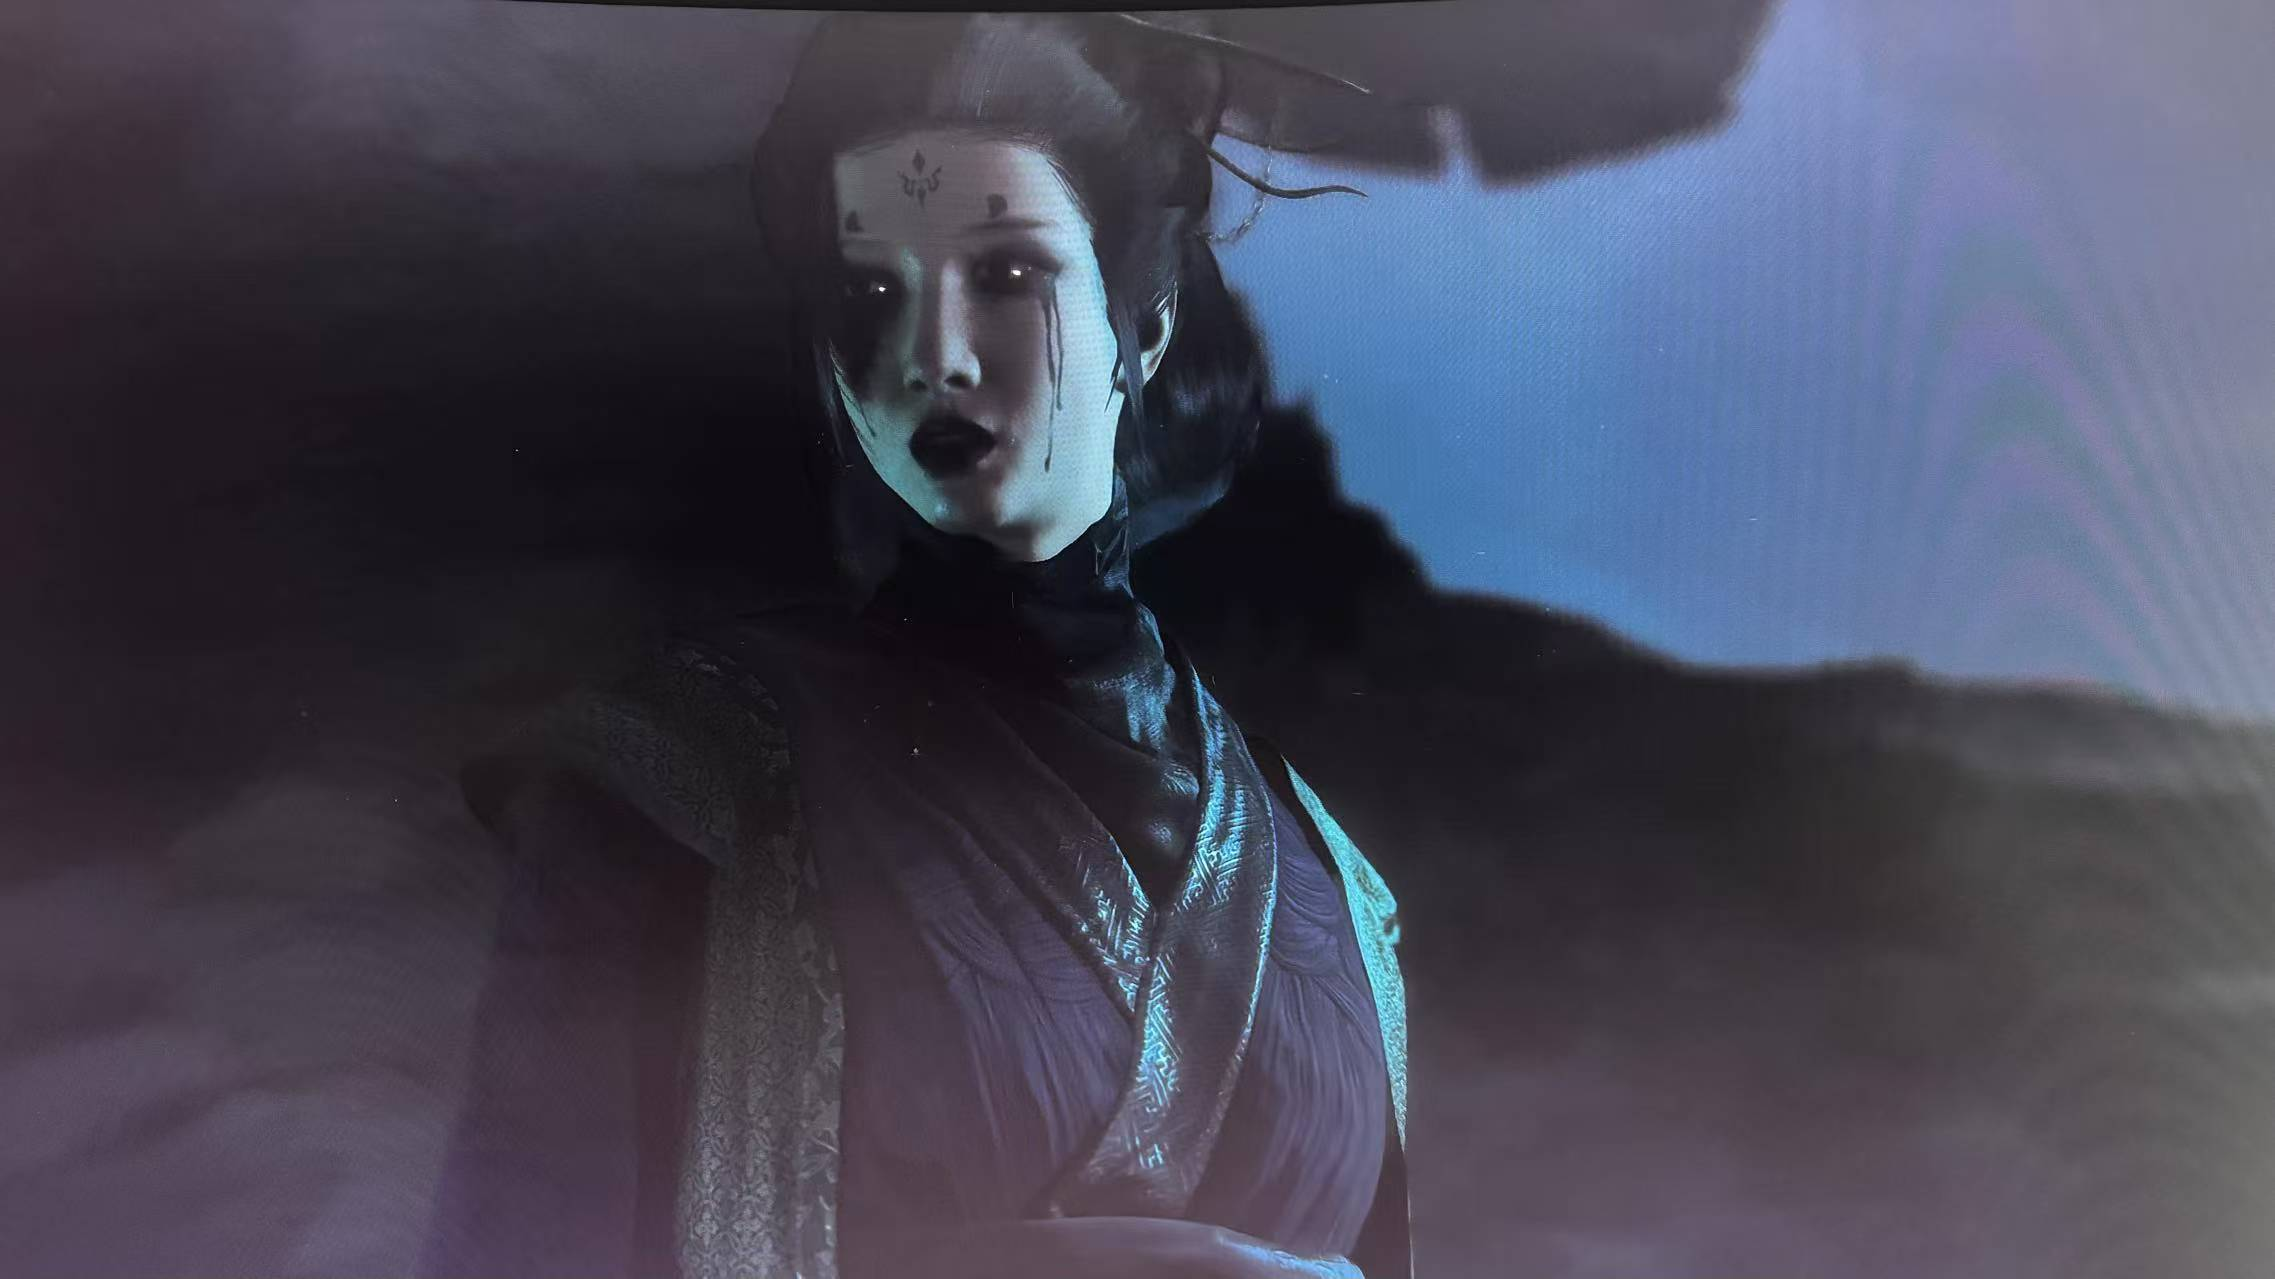
\includegraphics[width=0.7\textwidth]{pipeline.jpg}
\caption{Basic Rendering Pipeline}
\label{fig:pipeline}
\end{figure}

As shown in Figure~\ref{fig:pipeline}, rendering transforms 3D geometry into pixels.

---

% 代码示例

\section{Example Code}

C++ example:

\begin{lstlisting}[language=C++]
#include <iostream>

int main()
{
    std::cout << "Hello Game Dev!" << std::endl;
    return 0;
}
\end{lstlisting}

Python example:

\begin{lstlisting}[language=Python]
import pygame

pygame.init()

screen = pygame.display.set_mode((800,600))

running = True

while running:
    for event in pygame.event.get():
        if event.type == pygame.QUIT:
            running = False
\end{lstlisting}

---

%表格示例

\section{Common Game Engines}

\begin{table}[h]
\centering
\begin{tabular}{lll}
\toprule
Engine & Language & Type \\
\midrule
Unity & C\# & General \\
Unreal Engine & C++ & AAA \\
Godot & GDScript & Open Source \\
\bottomrule
\end{tabular}
\caption{Game engines comparison}
\end{table}

---

% 公式示例

\section{Basic Physics}

Velocity formula:

\[
v = \frac{dx}{dt}
\]

Newton's second law:

\[
F = ma
\]

---

% 提示框示例

\begin{tip}
Understanding vector math is essential for 3D graphics.
\end{tip}

\begin{warning}
Floating point precision errors can break physics simulations.
\end{warning}

---

%---------------------------------------------新章节

\chapter{蓝图编程}

\section{玩家移动}

关闭默认模板中的移动
\begin{itemize}
\item 更改“世界场景设置”中的“游戏模式重载”
\item 在“项目设置”，“地图和模式”中，更改“默认游戏模式”
\end{itemize}
新建移动：
\begin{itemize}
\item 新建蓝图类：游戏模式基础 BP\_GameMode
\item 新建蓝图类：角色 BP\_Charactor
\item 设置BP\_GameMode中默认pawn类为刚创建的角色BP\_Charactor，关联游戏模式和默认角色
\item 设置“项目设置”中的“地图和模式”中默认游戏模式为刚创建的BP\_GameMode
\item 新建文件夹Input用于处理输入，（不使用轴和操作映射，改用增强输入映射）
       \subitem 新建“输入”，“输入操作” IA\_Move2, 将“值类型”改为“Vector2D”
       \subitem 新建“输入”，“输入映射情景” IMC\_Input，在“映射”“Default Key Mappings”“Mappings”中添加IA\_Move2，绑定键盘WASD。向后走添加“修改器”，“否定”；左右走添加“修改器”，“拌合输入轴值”
\item 
\end{itemize}

\begin{figure}[h]
\centering
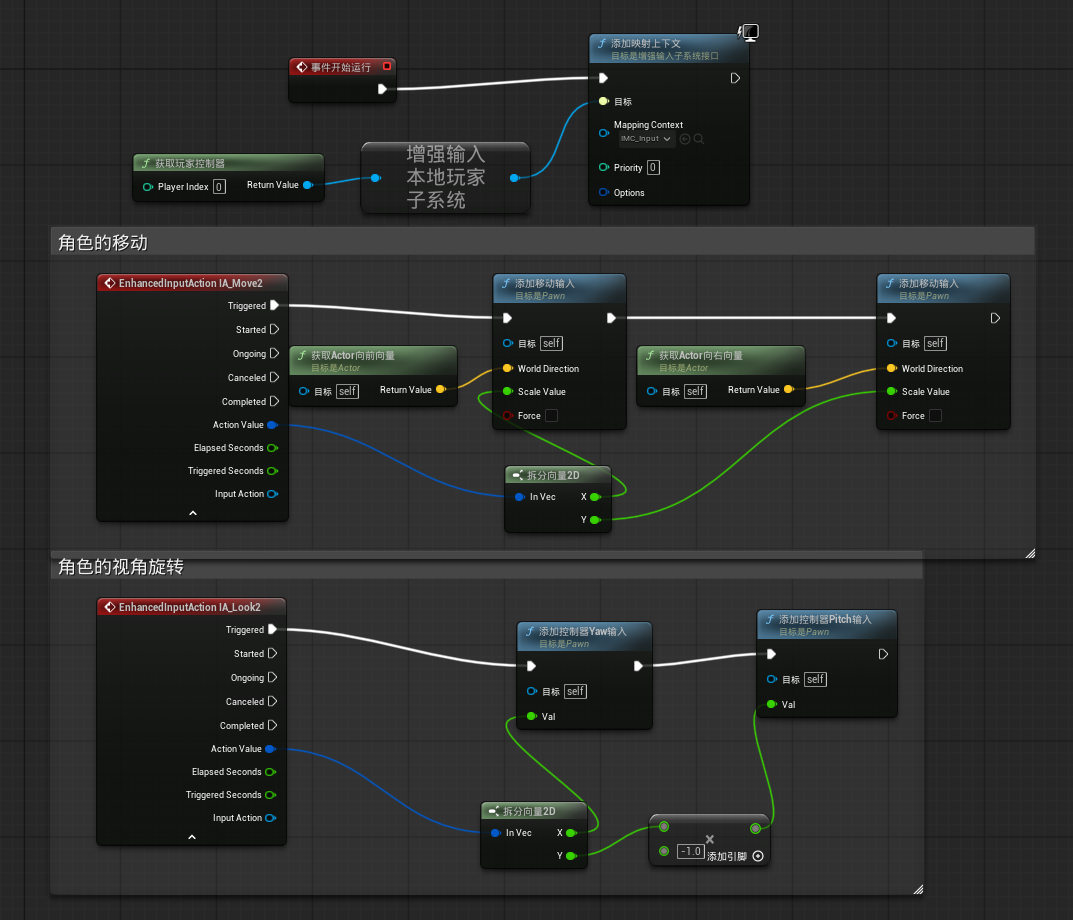
\includegraphics[width=1.0\textwidth]{BP_Charactor事件图表之移动.png}
\caption{BP\_Charactor事件图表之移动}
\end{figure}

\section{视角旋转}

新建鼠标旋转视角：
\begin{itemize}
\item 新建“输入”，“输入操作” IA\_Look2, 将“值类型”改为“Vector2D”
\item 修改 IMC\_Input，在“映射”“Default Key Mappings”“Mappings”中添加IA\_Look2，绑定鼠标XY 2D轴。
\item 姿态角 roll（横滚）、pitch（俯仰 y）、yaw（航向 x） 分别对应角色的前后、左右、上下旋转。
\item 上下移动时方向和惯用操作相反
      \subitem  法一：令值乘-1
      \subitem  法二：在IMC\_Input中，在IA\_Look2的“修改器”中添加修改器“否定”，且只勾选"Y"
\end{itemize}


\begin{tip}
框选蓝图按c，可以对蓝图进行注释
\end{tip}

\section{自动开关门功能}

新建开关门功能：
\begin{itemize}
\item 在“窗口”中选择“Fab”，添加一个门类型的资源
\item 修改门框的碰撞属性（默认为一个实心的门框，玩家无法通过），可在“光照”中“玩家碰撞”中查看物体的碰撞属性。在“碰撞”中选择“自动凸包碰撞”
\item 新建文件夹Door，添加Actor蓝图类BP\_Door，右上角添加两个静态网格体组件（模型），分别命名为DoorFrame和Door，DoorFrame设置为门框模型，Door设置为门模型（静态网格体选中指定资产）
\item 自动门用盒体碰撞实现，在“组件”中选择“Box Collision”，在“细节”中找到事件“组件开始/结束重叠时”添加逻辑
\item 使用时间轴组件，将一个值丝滑的过渡到另一个值（设置两个关键帧）
\end{itemize}


\begin{figure}[h]
\centering
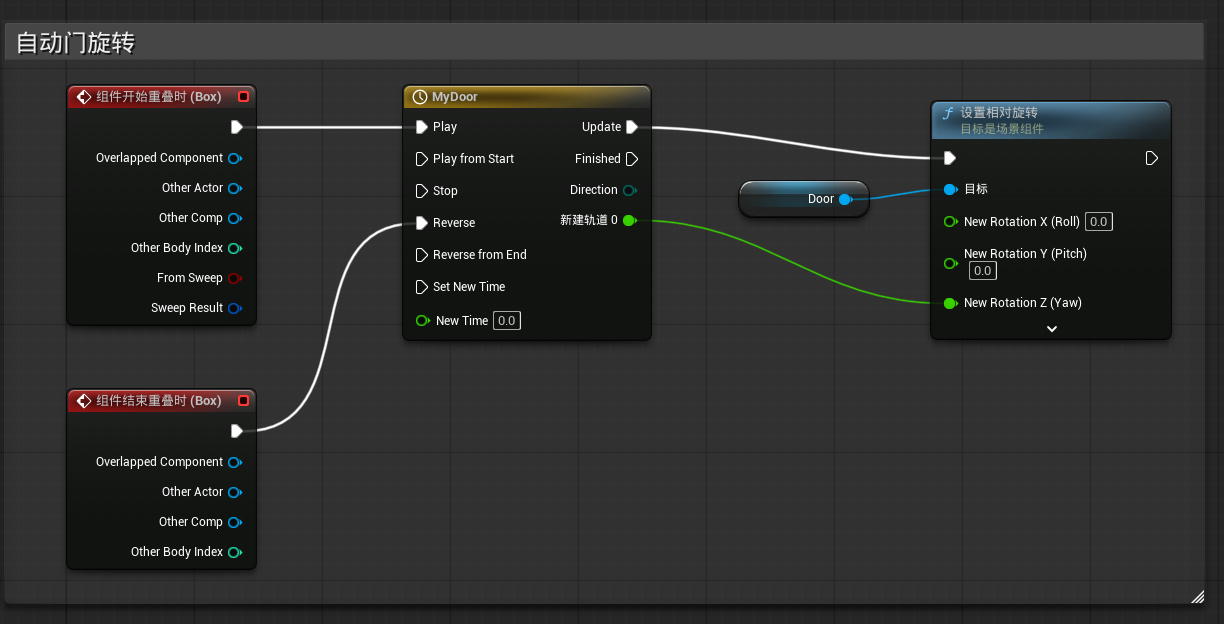
\includegraphics[width=1.0\textwidth]{BP_Door自动门旋转.png}
\caption{BP\_Door自动门旋转}
\end{figure}

\section{常用的流程控制节点}

常用的流程控制节点：
\begin{itemize}
\item 分支（Branch）：根据条件执行不同的分支    
\item FlipFlop：在两条路径之间切换执行，用法：下蹲按钮
\item doOnce：只执行一次，之后不再执行，除非reset，startclose是初始是的状态
\item 序列（Sequence）：按顺序执行多个节点，依次执行
\item 延迟（Delay）：在执行下一个节点之前等待指定的时间
\item ForLoop：循环执行节点，指定循环次数，左右都是闭区间
\item gate：根据条件控制执行，开关门的逻辑中，门打开(open)时执行路径打开，门关闭()时执行路径关闭,toggle时切换状态
\end{itemize}

\begin{figure}[h]
\centering
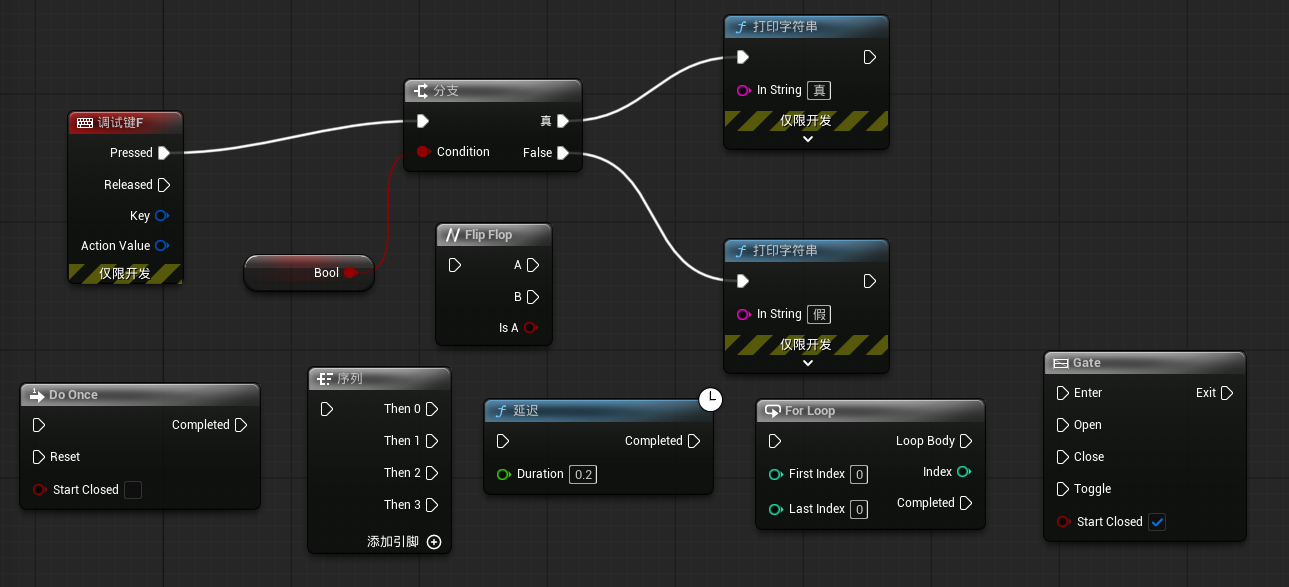
\includegraphics[width=1.0\textwidth]{7种常用的流程控制节点.png}
\caption{7种常用的流程控制节点}
\end{figure}

\section{第三人称动画系统}

制作第三人称运动系统：
\begin{itemize}
\item 选中BP\_Charactor，在“网格体”中添加一个骨骼网格体组件（带动画的模型），并调整正对的方向
\item 在组件中添加弹簧臂（SpringArm），并在这下面添加Camera，使角色在靠墙时视野不会穿透到墙里面
\item {\color{red} 在弹簧臂中，勾选“使用pawn”控制旋转，并选择角色类默认值，取消勾选“使用控制器旋转yaw”}
\item 修改蓝图，使角色的移动方向和摄像机的方向一致
\item 在类默认值中，角色移动（旋转设置）中，勾选“将旋转朝向运动”

\end{itemize}


\begin{figure}[h]
\centering
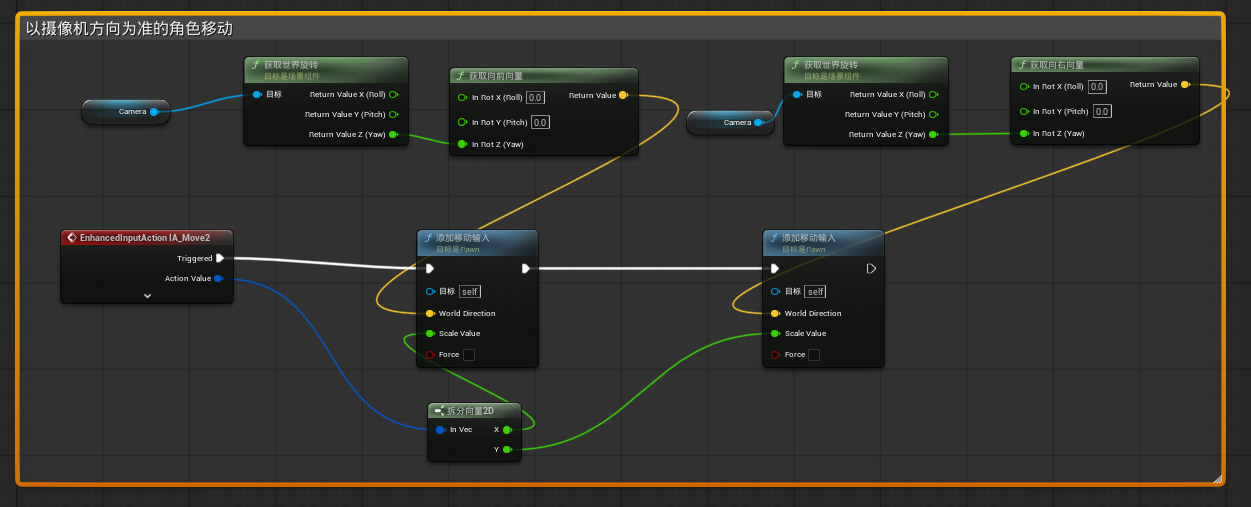
\includegraphics[width=1.0\textwidth]{角色移动逻辑（摄像机）.png}
\caption{角色移动逻辑（摄像机}
\end{figure}

制作第三人称动画系统：
\begin{itemize}
\item 新建Animation文件夹，新建动画->动画蓝图 ABP\_Main,新建动画->混合空间 BS\_Walk
\item 混合空间：混合两个不同的动画，让动画间能进入丝滑的过渡；设置平滑时间0.2,平滑类型为立方，使停止时更加丝滑
\item 在ABP\_Main中设置浮点型变量Speed，依据Speed的值传入混合空间，实现动画的切换
\item 在BP\_Charactor中，类默认值->动画->动画蓝图，选择ABP\_Main
\end{itemize}

\begin{figure}[h]
\centering
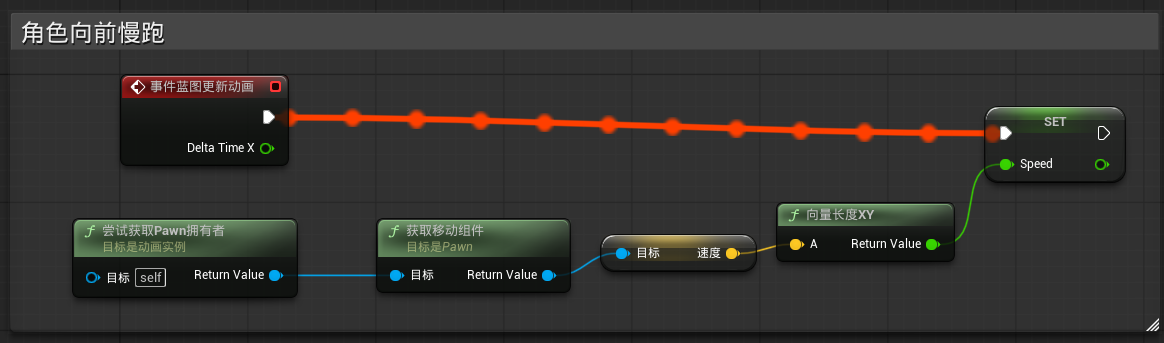
\includegraphics[width=1.0\textwidth]{角色移动动画蓝图.png}
\caption{角色移动动画蓝图}
\end{figure}

%---------------------------------------------新章节
\chapter{蓝图实战}

\section{第二章复习}

\begin{itemize}
\item 在epic games中找到虚幻引擎->库，找到我的项目中的ChallengeGame，右键“在文件夹中显示”，在content下导入素材
\item Maps->关卡，Materials->材质，Meshes->模型，Textures->纹理
\item 在Code->Character->Input下，新建输入操作IA\_Move，IA\_Look，IMC\_Challenge
\item 新建游戏模式基础BP\_ChallengeMode，将项目默认游戏模式更改为BP\_ChallengeMode，并设置默认pawn类为BP\_ChallengeCharacter，同时给BP\_ChallengeCharacter添加骨骼网格体组件，弹簧臂组件和摄像机组件
\item 实现角色移动和视角旋转的逻辑（F2.1），在弹簧臂中，勾选“使用 pawn”控制旋转，并选择角色类默认值，取消勾选“使用控制器旋转 yaw”，勾选“将旋转朝向运动”
\item 添加动画过渡，混合空间采用旧有->1D即可，（F2.5）
\end{itemize}

\begin{tip}
选中蓝图组件按alt，可以查看该组件的英文名称
\end{tip}


\begin{tip}
悬浮在线条上双击，可以理线
\end{tip}

\begin{tip}
混合空间中，按住ctrl拖动进度条，可以显示动画预览
\end{tip}

\begin{figure}[h]
\centering
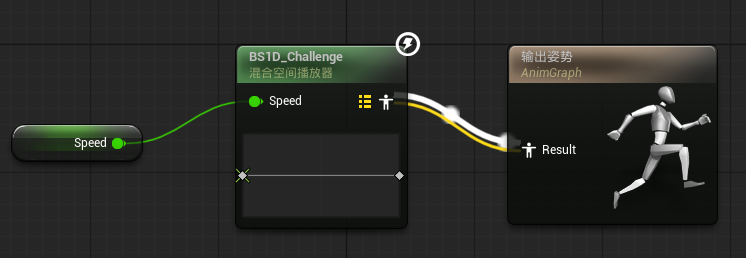
\includegraphics[width=1.0\textwidth]{使用混合空间.png}
\caption{使用混合空间，结合图2.5使用}
\end{figure}

\section{实现跳跃功能}

\begin{itemize}
\item 增加输入操作IA\_Jump，绑定空格键，值无需修改（数字）。因为跳跃按一下就会执行一次，不需要长时间按所以不需要轴输入。
\item 角色事件图中添加逻辑，当IA\_Jump被触发时，调用角色的Jump函数（角色类自带的函数），{\color{red} 使用started连，而不用trigger连}
\item 制作跳跃动画，引入状态机(F3.1)。给每一个状态添加动画，并添加转化条件
\subitem locomotion->Jump\_Start->角色不在地面上且有向上的速度，此时1.需要分割z轴速度 2.使用类型转换节点将父类pawn转换为子类BP\_ChallengeCharacter，得到isFalling变量（F3.3）
\subitem Jump\_Start->Jump\_Loop->Jump\_Start动画即将播放完成（F3.4）
\subitem Jump\_Loop->Jump\_End->角色在地面上 (F3.5)
\subitem Jump\_End->locomotion-> 角色重新走动或者重新跳跃。假设角色跳跃后没有走动，又再次跳了一下，只有speed >= 1的判断条件的话
，没有令角色转回locomotion，导致第二次跳跃动画没有播放（F3.6)


\end{itemize}



\begin{tip}
在状态机节点上，拖动边缘可以引出线，拖动中间可以移动节点
\end{tip}

\begin{warning}
若在设置状态机状态时，动画为绿色，则无法编译。需要将该动画"附加设置"->additive动画类型改为“无additive”
\end{warning}

\begin{tip}
事件图中，选中连线按alt，可以切断该连线
\end{tip}

\begin{figure}[h]
\centering
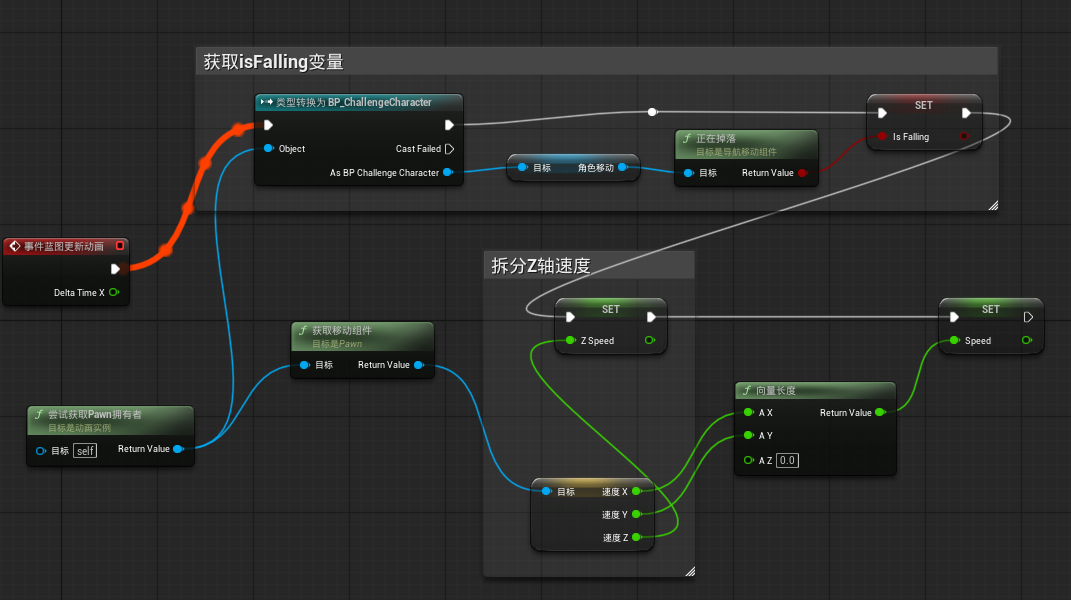
\includegraphics[width=1.0\textwidth]{获取角色更多信息.png}
\caption{获取角色z轴速度以及是否掉落}
\end{figure}

\begin{figure}[h]
\centering
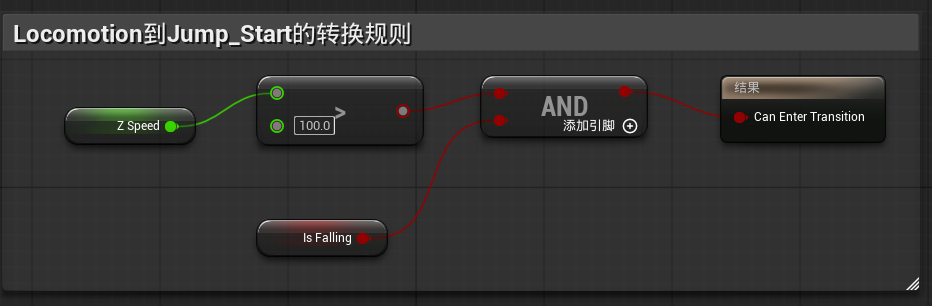
\includegraphics[width=1.0\textwidth]{转换规则1.png}
\caption{转换规则1}
\end{figure}

\begin{figure}[h]
\centering
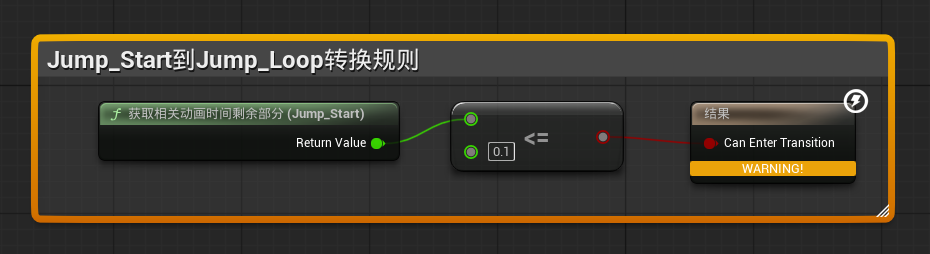
\includegraphics[width=1.0\textwidth]{转换规则2.png}
\caption{转换规则2}
\end{figure}

\begin{figure}[h]
\centering
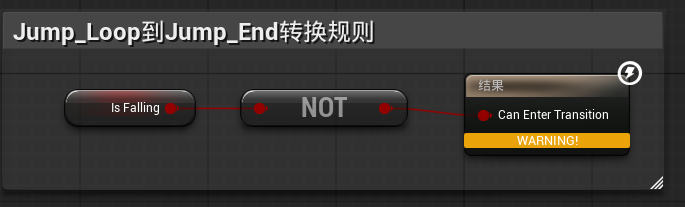
\includegraphics[width=1.0\textwidth]{转换规则3.png}
\caption{转换规则3}
\end{figure}

\begin{figure}[h]
\centering
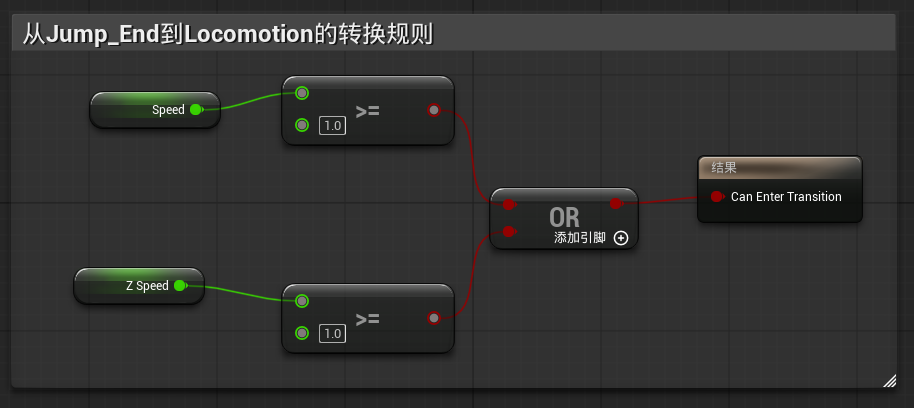
\includegraphics[width=1.0\textwidth]{转换规则4.png}
\caption{转换规则4}
\end{figure}


\begin{tip}
调试时，小窗显示状态机，并选中已生成的运行示例，可以实时查看状态
\end{tip}

\section{实现场景机关陷阱--大摆锤动画}

bug修复：上一节的Jump\_End->locomotion转换逻辑中，只有角色重新运动（有速度）才会转换回去，这意味着
假设我们跳跃完不动，则角色一直卡在Jump\_End，静止不动。\\
解决方法：添加一个条件，若剩余动画的播放时间小于0.1秒，则转换回locomotion。

\begin{itemize}
\item 在Code中新建文件夹Mechanism，保存机关陷阱,新建Actor蓝图类BP\_Sphere(大摆锤陷阱)
\item BP\_Sphere左上角添加“静态网格体组件”（即模型）Sphere，在“细节”中选择模型
\item 添加一个球形碰撞组件SphereCollision为模型的子类，调整大小使其包裹住模型
\item 在事件图中，添加逻辑，添加时间轴，并创建浮点型轨道，设置三个关键帧，控制大摆锤pitch(y轴)角度从左摆到右，再从右摆到左，并右键关键帧选择“自动”，使其过渡更加丝滑
\item 使用自定义事件实现无限循环


\end{itemize}


\begin{tip}
选中事件图中的组件，按F2，可以更改名称
\end{tip}

\begin{figure}[h]
\centering
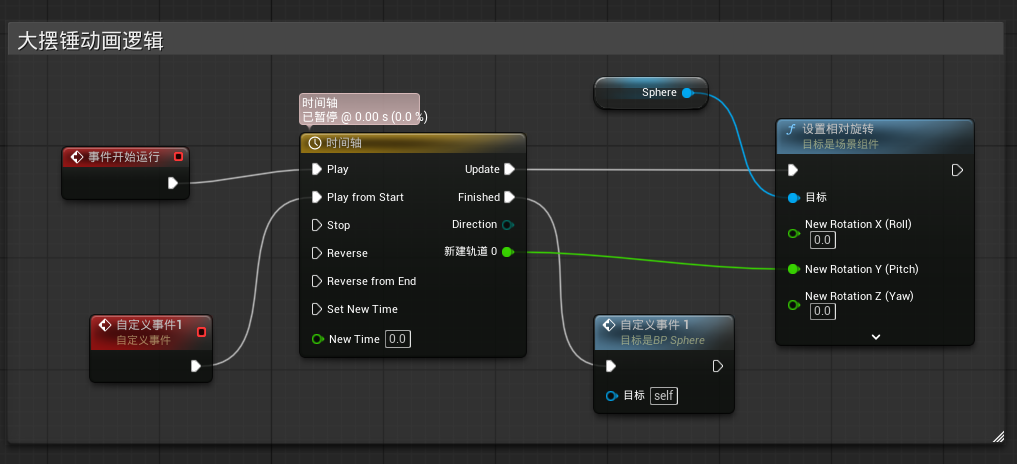
\includegraphics[width=1.0\textwidth]{大摆锤动画逻辑.png}
\caption{大摆锤动画逻辑}
\end{figure}

\section{实现角色死亡布娃娃效果}

\begin{itemize}
\item 在角色BP\_ChallengeCharactor事件图中，定义死亡事件
\item 在大摆锤BP\_Sphere事件图中，添加碰撞逻辑，当角色与球形碰撞组件发生重叠（在碰撞中找到该事件）时，调用角色的死亡事件
\item 双击角色的骨骼网格体组件，在“物理”导入物理资产
\item 此时角色被撞后，直接消失了（掉到地面之外去了） -> 将网格体“碰撞”改为PhysicsActor，使角色会和地面碰撞
\item 角色被撞后，摄像机直接自由了 -> 将摄像机的父类弹簧臂挂载到网格体下面
\item 摄像机可能会卡住 -> 在弹簧臂组件中，取消勾选“摄像机碰撞”“进行碰撞测试”，使摄像机不会穿透物体 或 使用事件图实现
\item 为了保险起见，死亡后设置运动模式为“无”
\end{itemize}

\begin{figure}[h]
\centering
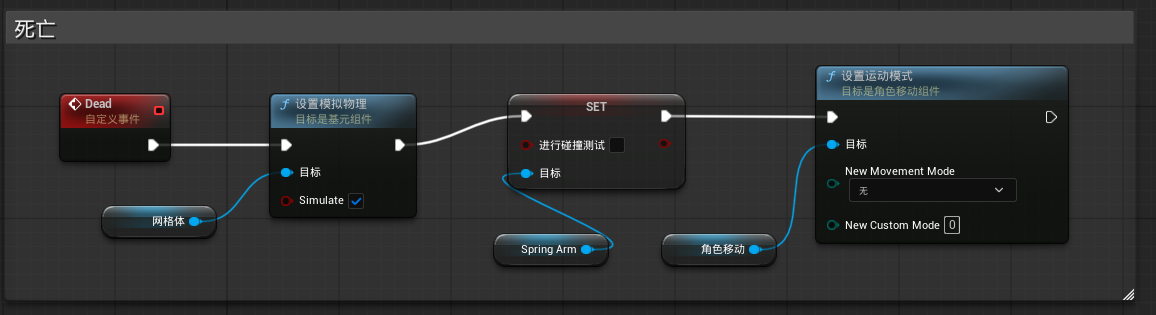
\includegraphics[width=1.0\textwidth]{角色死亡逻辑.png}
\caption{角色死亡逻辑}
\end{figure}

\section{实现角色死亡后重生逻辑}

\begin{itemize}
\item 角色死亡后，首先延迟几秒，接着销毁当前actor（角色是actor的一个子类），最后调用重生逻辑在检查点生成一个新的角色
\item 重生逻辑（BP\_ChallengeMode中实现）：使用“生成actor”节点，类选择我们的角色，并设置重生位置。新建“变换”类变量RebirthLocal，分割结构体引脚，连接位置与旋转（无需连接缩放）
\subitem 设置检查点变量的原因是因为在不同的位置死亡有不同的检查点，该变量需要由外部实时更新 

\end{itemize}

\begin{figure}[h]
\centering
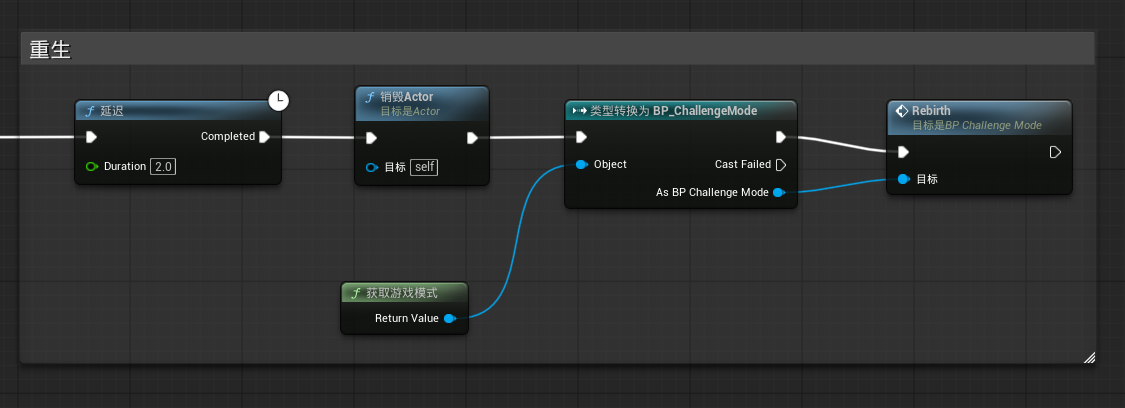
\includegraphics[width=1.0\textwidth]{角色重生.png}
\caption{角色重生}
\end{figure}

\begin{figure}[h]
\centering
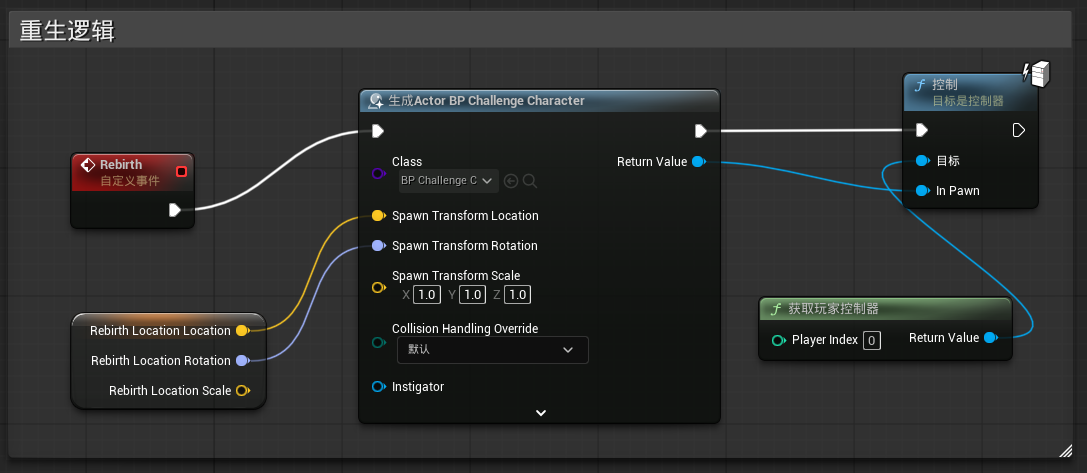
\includegraphics[width=1.0\textwidth]{重生逻辑.png}
\caption{重生逻辑}
\end{figure}


%---------------------------------------------新章节

\chapter{数学运算}

\section{运算符}

\begin{itemize}
\item 加法：add
\item 减法：subtract
\item 乘法：multiply    
\item 除法：divide
\item 灰色引脚，通配符 -> 可以连接任意类型的输入输出
\item 平方：square
\item 平方根：sqrt
\item 幂：power 
\item 取余：modulo \%
\item 绝对值：abs
\item 数学表达式：expression 通过输入字符串的方式在名称处输入表达式，使用输入引脚传入变量。通常使用数学表达式即可，他会自动生成其他节点
\end{itemize}


\begin{warning}
加法乘法满足交换律，顺序不影响结果；减法除法不满足交换律！
\end{warning}

\section{向量}


\begin{itemize}
    \item 坐标 -> 位置
    \item 方向 + 程度（模长，代表速度，力度）
    \item 向量的点积 -> 判断向量的相对方向，使用dot计算，结果属于[-1,1]-> 可以用于背刺处决 :当结果接近1时，说明两个向量方向相同，即角色从后方正对敌人；当结果接近-1时，说明两个向量方向相反，即角色与敌人面对面；

\end{itemize}



%---------------------------------------------新章节

\part{开放世界开发}

\chapter{人物系统}

\section{移动}

大纲
\begin{itemize}
    \item 创建第三人称新项目 RPG\_TuTorial\_Series，选择蓝图与第三人称模板
    \item 在Charactor文件夹中，新建RPG\_Charactor,新建动画Animations,新建状态Locomotion（移动）和Crouched（蹲伏）
    \item 设置Locomotion，Jump，Crouched的动画，并设置状态转换
    \item Crouched动作需要添加新的输入映射（左ctrl键），蹲伏后角色速度更慢，视角更远
    \item 加入倾斜动作，
    \subitem 添加lean文件夹与两个动画，均为Run\_Fwd的副本
    \subitem 设置为叠加（Additive）动画类型为“网格体空间”，基础姿势类型为“选择的动画缩放”,并选择Run\_Fwd作为基础动画
    \subitem 进入骨骼树，选中骨盆，旋转10°，保存关键帧
    \subitem 新建Lean混合空间，水平坐标设为Lean Value，左侧选中左倾动画，右侧选中右倾动画，并与走路动画进行混合
    \subitem {\color{red} 困难！}在角色动画蓝图中，添加Lean Value变量，并计算倾斜值，逻辑如(F5.4)所示，计算每一帧角度和上一帧角度的差值
    \item 更改人物的材质，改变颜色为蓝色
    \item 给项目增加版本控制 -> 一直push失败，从https改用ssh -> 仍然不行，单次上传的文件不可以超过2GB
\end{itemize}

操作要点：
\begin{itemize}
\item idle->walk/run->stop，Speed为0时转换到idle，Speed大于0时转换到walk/run，Speed小于等于0时转换到stop，stop到idle只需勾选{\color{blue} 基于状态中序列播放器的自动规则}，即stop动画结束，会自动跳转到idle。
\item 添加跳跃状态机：Jump->Falling（勾选循环动画）
\item 设置Land为叠加播放（Additive），与缓存的locomotion叠加，实现跳跃时角色仍然有行走的动画
\item 角色的跳跃动画好像被吞掉了-->从To Falling到跳跃与降落的优先级相同，我们令跳跃的优先级更高（1最高）
\item 蹲伏后角色的速度更慢 -> 设置角色移动中最大行走速度为350（奔跑为500）
\item 蹲伏后镜头要拉远 -> 设置弹簧臂的目标臂长为550（正常为400）-> 画面会因为相机位置突然跳变，实现平滑过渡需要添加时间轴组件，设置两个关键帧(0,0)(1,1),连接插值（lerp）插件 
\end{itemize}






\begin{tip}
可以使用添加状态别名的方式来使逻辑更加清晰
\end{tip}


\begin{tip}
对动画图中，全部选中按Q可以对齐
\end{tip}


\begin{figure}[h]
\centering
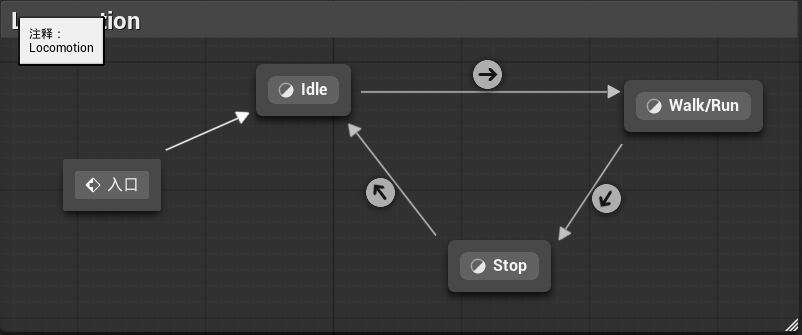
\includegraphics[width=1.0\textwidth]{Locomotion逻辑.png}
\caption{Locomotion逻辑}
\end{figure}

\begin{warning}
在绑定了蹲伏按键后，按左control没有任何反应，我编译检查状态，发现没有进入IA\_Crouch分支。后续检查发现，按任何除了wasd空格的案件均没有反应。
经过层层排查，最终发现使用的IMC\_Default为同名，不同路径下的另一个输入映射情景，但是更改完WASD不再能使用->character中事件图调用的增强输入均为另一个路径下的文件
\end{warning}

\begin{warning}
按下了蹲伏以后，如果直接跳跃不会解除蹲伏状态 -> 在跳跃逻辑中，如果没有蹲伏，就直接跳跃；如果蹲伏了，则翻转蹲伏，再跳跃
\end{warning}

\begin{figure}[h]
\centering
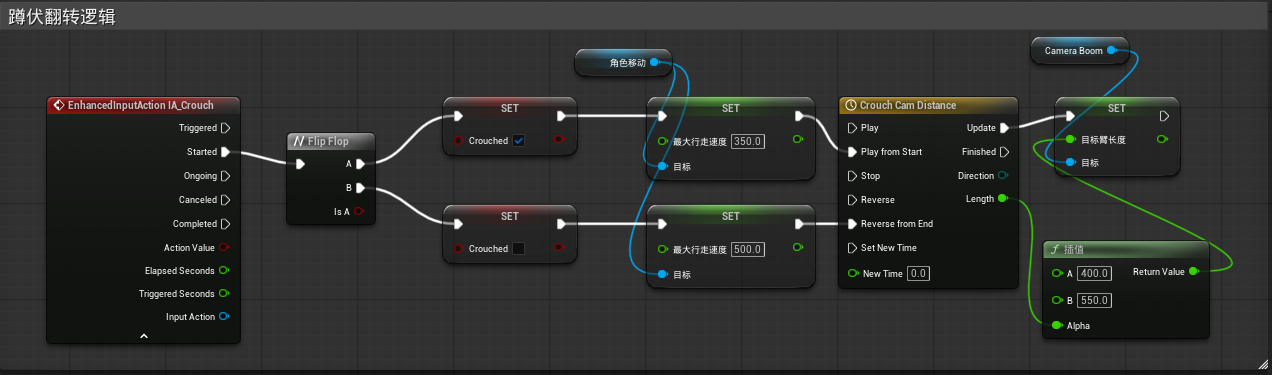
\includegraphics[width=1.0\textwidth]{蹲伏翻转逻辑.png}
\caption{蹲伏翻转逻辑}
\end{figure}

\begin{figure}[h]
\centering
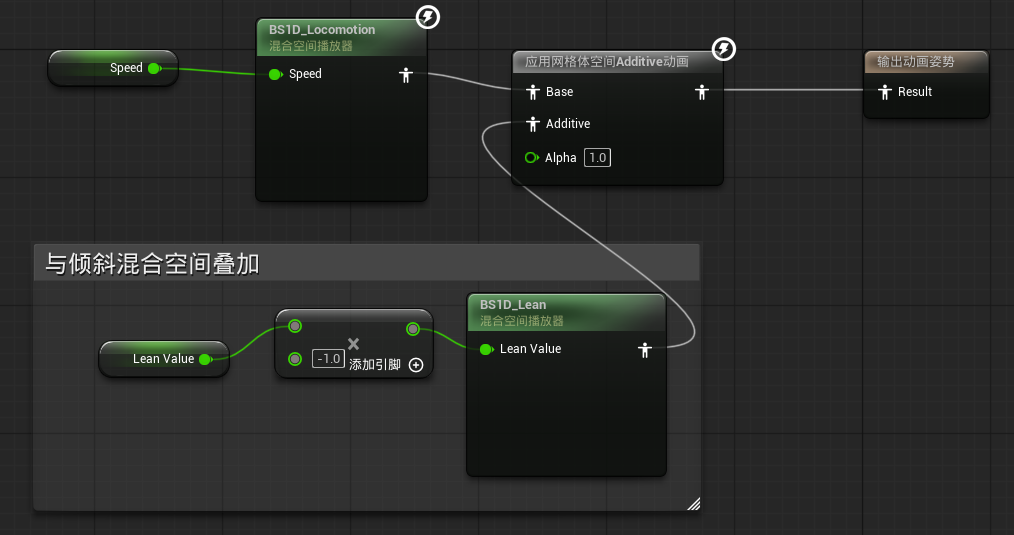
\includegraphics[width=1.0\textwidth]{修改走路动画.png}
\caption{修改走路动画，与倾斜动画叠加使用}
\end{figure}

\begin{figure}[h]
\centering
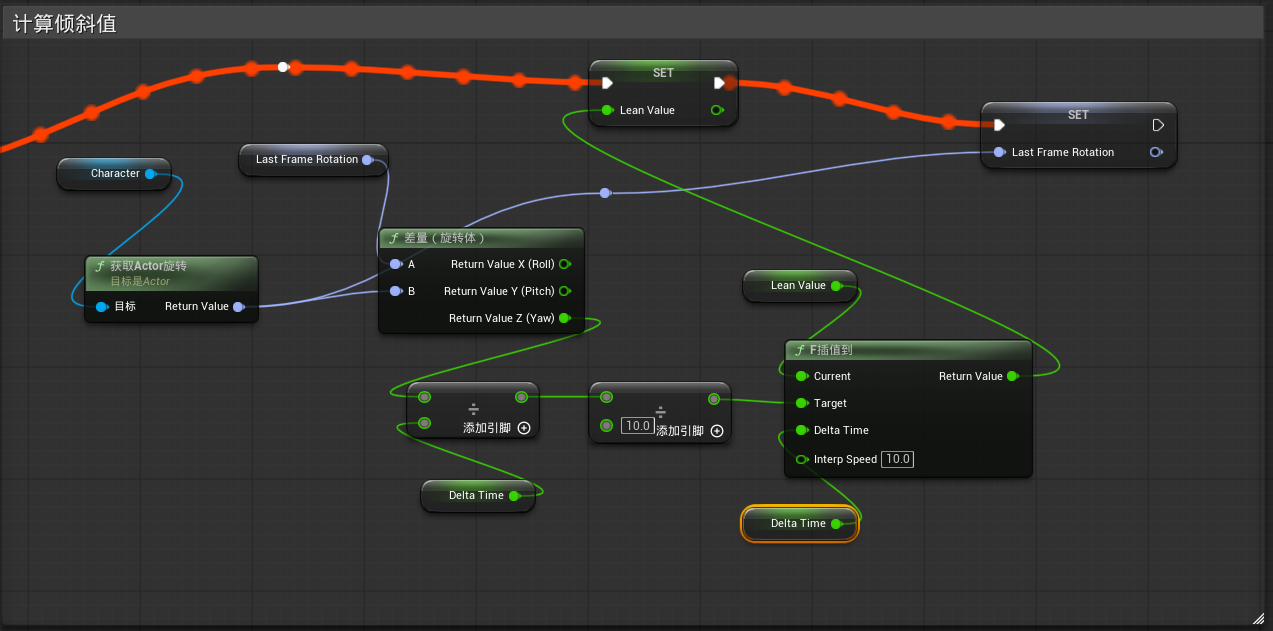
\includegraphics[width=1.0\textwidth]{计算倾斜值.png}
\caption{计算倾斜值}
\end{figure}




\section{动态扭曲翻越}


\begin{itemize}
    \item “编辑”“插件”中，添加motion warping插件
    \item 动画中新建Vaulting文件夹，导入翻越动画，启用“根骨骼运动”
    \item 选中翻越动画，右键选择“创建动画蒙太奇”，新建蒙太奇
    \item 在蒙太奇动画通知轨道右键“添加通知状态”“添加运动扭曲”，按住shift拖动选取范围，可以显示实时帧
    \item 双击MontionWarping，修改“忽略z轴”“扭曲旋转”部分
    \item 进入人物蓝图，首先添加运动扭曲组件，接着创建新函数Vault，与Vault Motion Warp事件
\end{itemize}

操作要点：
\begin{itemize}
    \item 翻越函数的实现首先需要启用至多三次球形射线追踪，球形射线彼此相距30个单位，从目标点平行指向前方。
    \item 一旦球形射线追踪命中，再依据命中位置，垂直于地面发出6条射线，表示需要翻越的距离。
    \item 设置变量起始翻越位置Vault Start Pos并debug球，垂直射线与击中物体的第一个交点就是起始翻越位置
    \item 设置变量中部翻越位置Vault Middle Pos并debug球，保存6条垂直射线中与物体相交的点
    \item 设置变量结束翻越位置Vault Land Pos，保存6条射线中第一条不与物体相交的线，在这条线一段距离后就是着陆点线
    \item 将起点、中点、着陆点传入蒙太奇的运动扭曲通知状态，完成动态扭曲翻越
    \item 修改输入为增强输入，连出Started引脚

\end{itemize}

\begin{tip}
可以对变量创建类别，使变量列表更加清晰
\end{tip}

\begin{warning}
按了shift后播放了动画，但是看起来没有丝毫位移 -> 在触发 Vault Motion Warp事件时，没有将运动模式设置为“正在飞行”
\end{warning}

\begin{warning}
观察蹲伏状态，感觉人物蹲的太快了点，但这是状态间的转化 -> 状态间的转化由引擎自动blend生成 -> 修改转换条件“混合设置”时长为0.5s
\end{warning}

\begin{figure}[h]
\centering
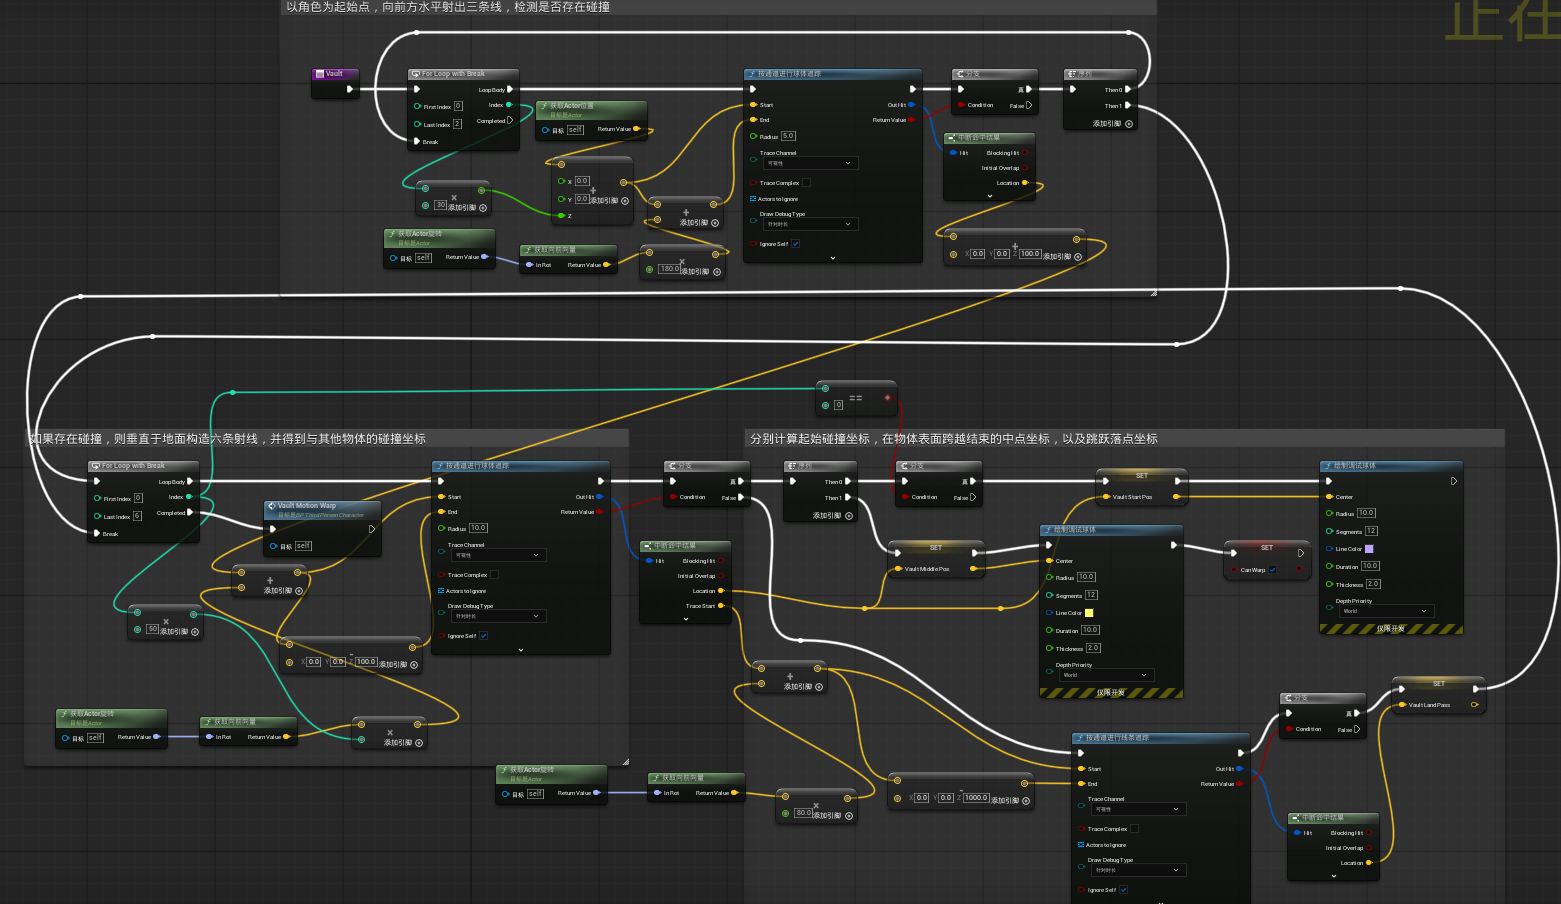
\includegraphics[width=1.0\textwidth]{翻越逻辑.png}
\caption{翻越逻辑}
\end{figure}


\begin{figure}[h]
\centering
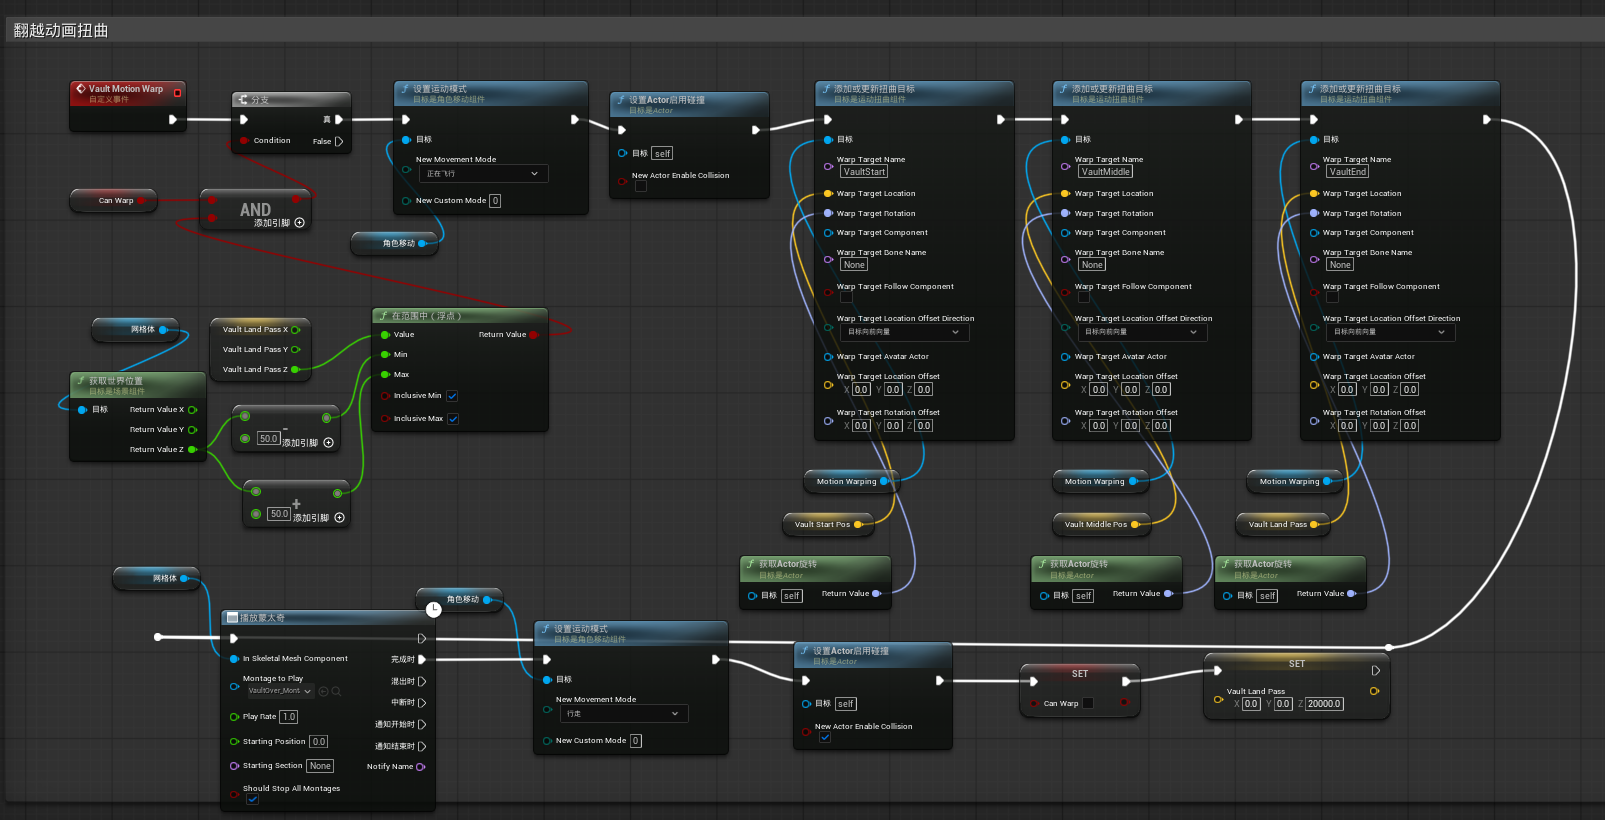
\includegraphics[width=1.0\textwidth]{翻越动画扭曲.png}
\caption{翻越动画扭曲}
\end{figure}

\section{暗杀}

\begin{itemize}
    \item 在动画文件夹下新建Assassinations，存放暗杀动作,同上一节，为两个暗杀动画(攻击和受击)启用根运动，并创建蒙太奇
    \item 创建输入映射，绑定按键F
    \item 新建文件夹BluePrints,在里面创建蓝图接口BPI\_Assassination;创建测试类假人BP\_Dummy,并添加球形碰撞,在“类设置”中添加接口
    \item 给测试类假人BP\_Dummy添加一个网格体作为模拟目标，并且保证他没有启用碰撞预设，且游戏中不可见
    \item 添加攻击与受击逻辑
    \item 敌人被刺杀后进入布娃娃状态,将碰撞预设改为“Customer”，取消勾选相机，将胶囊体组件的碰撞预设改为"IgnoreOnlyPawn"
    \item 新建UI文件夹，新建“用户界面”“控件蓝图”，做一个刺杀提示,在BP\_Dummmy中添加widget组件
\end{itemize}

\begin{figure}[h]
\centering
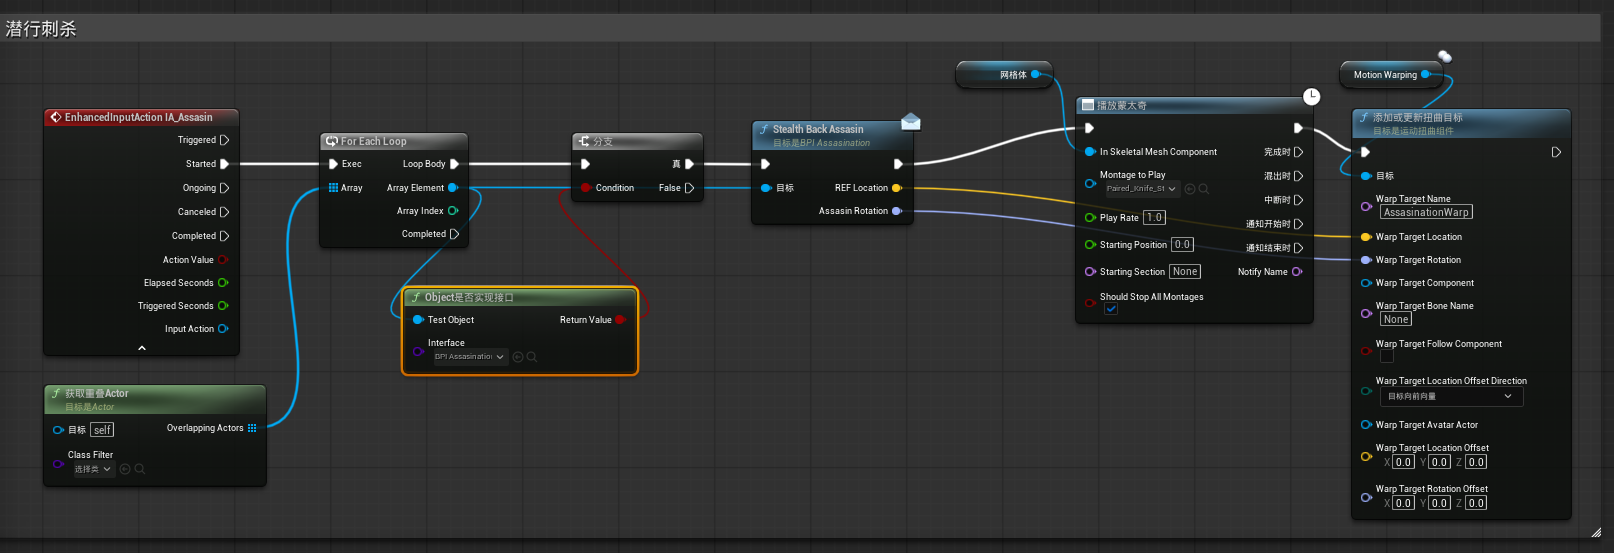
\includegraphics[width=1.0\textwidth]{刺杀逻辑.png}
\caption{刺杀逻辑}
\end{figure}

\begin{figure}[h]
\centering
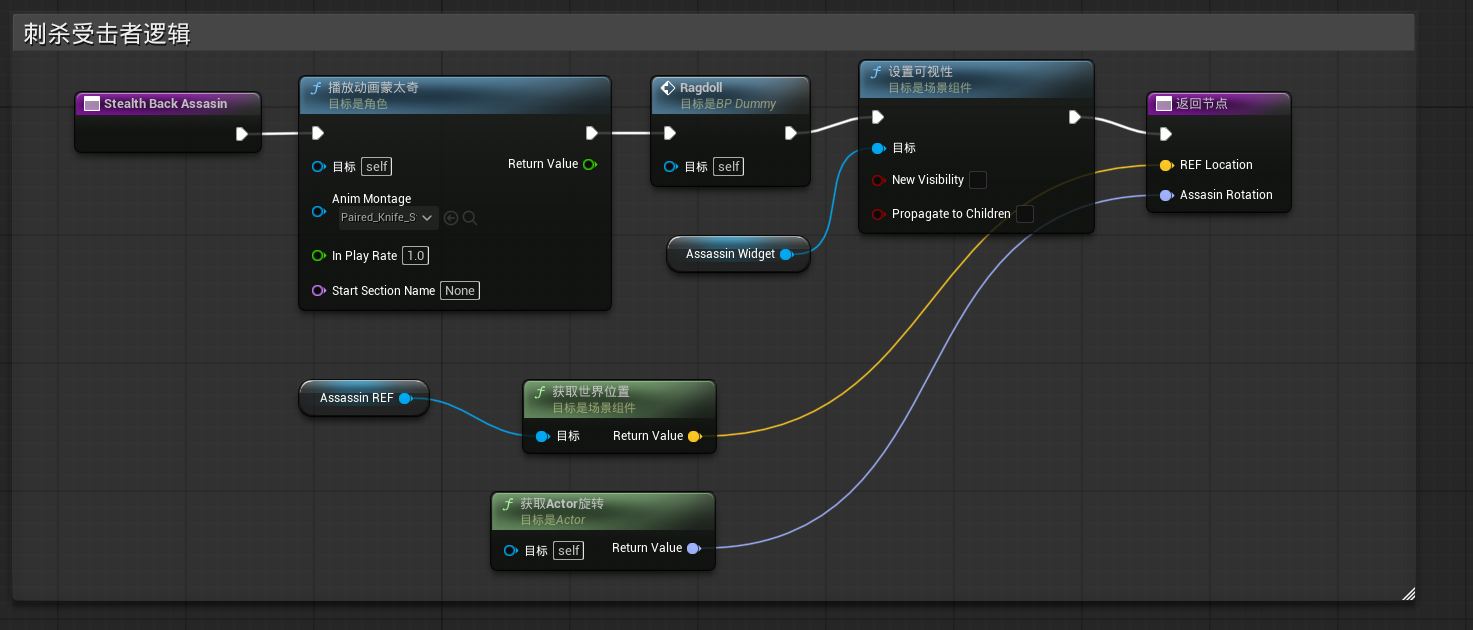
\includegraphics[width=1.0\textwidth]{假人受击逻辑.png}
\caption{假人受击逻辑}
\end{figure}

\begin{figure}[h]
\centering
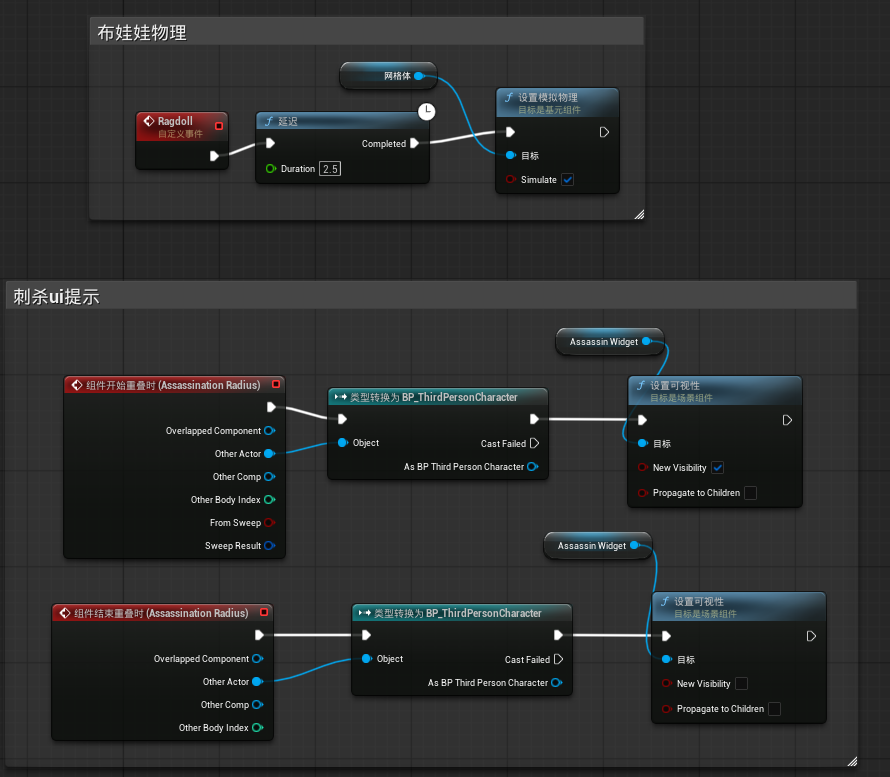
\includegraphics[width=1.0\textwidth]{刺杀UI提示.png}
\caption{刺杀UI提示}
\end{figure}


\begin{figure}[h]
\centering
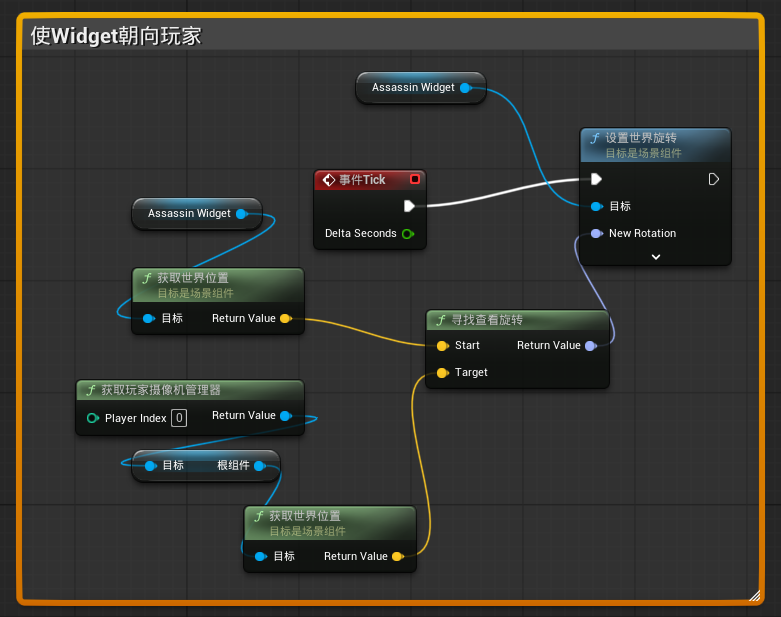
\includegraphics[width=1.0\textwidth]{自动调整文字提示朝向.png}
\caption{自动调整文字提示朝向}
\end{figure}


%---------------------------------------------新章节
\section{玩家属性}

\begin{itemize}
    \item 在Blueprints添加Actor component蓝图类BPC\_Player Stats,添加属性生命值，耐力值，经验等属性，设定默认值，实现增加与减少函数
    \item 在UI中添加UserWidget WB\_HUD，添加血条与耐力条,在人物蓝图中事件开始时调用该部件。
    \item 血量使用进度条,设置锚点调整位置，为百分比创建绑定（每一帧读取）或当属性改变时传入；血条上添加文本框
    \item 编写血量增加减少逻辑（F5.12）并且在血量变化时更新相关变量，在角色控制蓝图中添加BPC\_Player Stats组件
    \item 启用组件“事件任意伤害”，调用血量减少逻辑
    \item 实现死亡事件：禁用输入，对角色网格体设置模拟物理（布娃娃），并设置mesh碰撞预设为自定义，启用碰撞（查询和物理），胶囊体碰撞预设改为“仅忽略pawn”（否则自身网格体会与胶囊体发生碰撞）
    \item 实现耐力系统后，创建新按键冲刺（左alt），按住冲刺键将最大速度由500改为1000，并消耗耐力。耐力降为0以后，不允许跑步,使用定时器实现相关逻辑（F5.14）。
    \item 当角色速度没有冲刺时，令耐力逐渐恢复，这个检查逻辑通过event tick每一帧检查一次 ，因此自带循环逻辑，不用通过事件实现
    \item 修复角色在蹲下时可以奔跑bug，增加冲刺动画（将原来的跑步动画速率调高），并添加进入locomotion的混合空间（多加个关键帧）
    \item 增加经验值与等级系统，制作经验值UI ，操作与之前类似
    \item 创建新文件夹Audio放置音效，Footsteps（脚步声），Grunts-Hit（呻吟声和击打声）,UI（界面类声音 ）
    \item 以脚步声为例，新建Meta Sound Source，添加音效的随机扰动。并创建声音衰减资产，防止声音的无限传播 。Inner Radius（内半径）内声音为百分百，Falloff Distance（衰减距离）控制衰减曲线，脚步音和源声音都需要应用衰减。
    \item 将声音应用到动画源，进入通知新增轨道，在关键帧右键“新建状态”“播放声音”

\end{itemize}

操作要点：
\begin{itemize}
    \item 血量下降时，不能令血量为负数 -> 在减少血量函数中，首先判断当前血量是否小于等于0
    \item 跑步使用普通的声音即可，落地时使用metasound，并乘一个适当的系数
    \item 角色死亡后再播放死亡音效延迟过长，我们可以使用Sequence节点让逻辑同时执行
    \item 新建Sound Cue，实现死亡的随机音效（多种音效随机选取一个）
    \item 修复角色未移动，按住alt仍然消耗耐力的bug 

\end{itemize}


\begin{figure}[h]
\centering
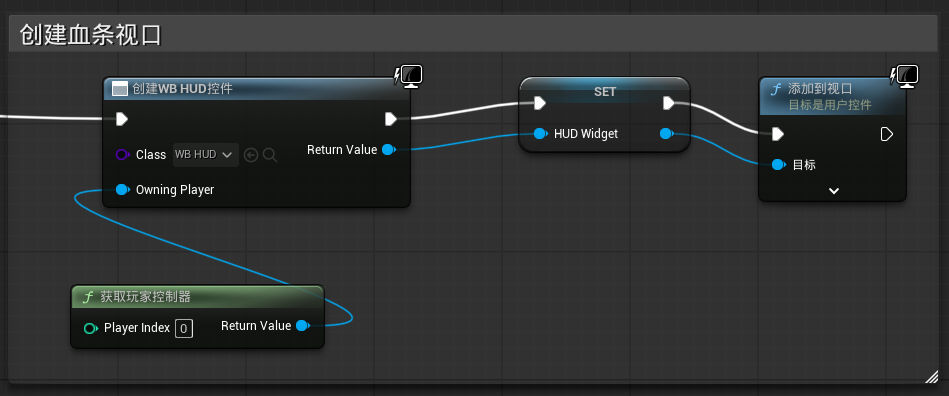
\includegraphics[width=1.0\textwidth]{调用血条组件.png}
\caption{调用血条组件}
\end{figure}


\begin{figure}[h]
\centering
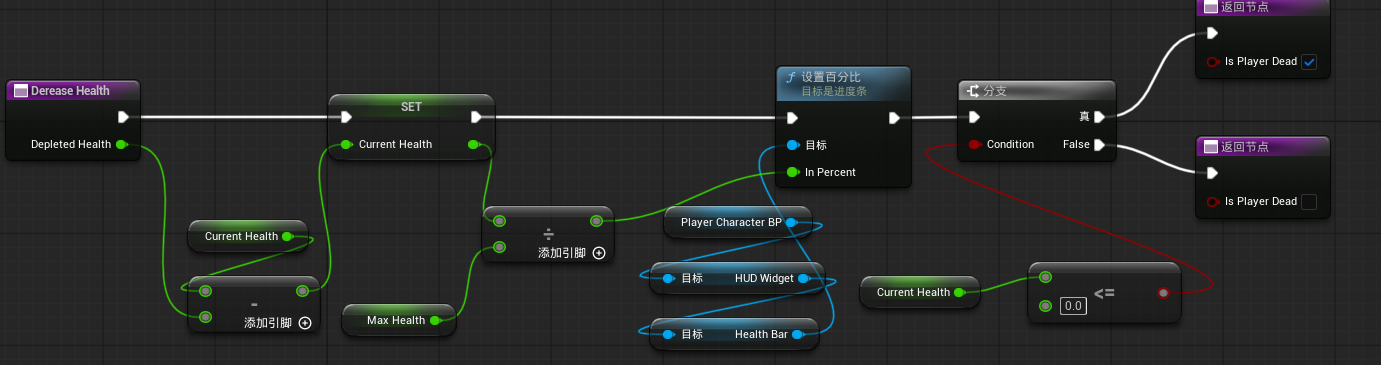
\includegraphics[width=1.0\textwidth]{血量减少ui显示.png}
\caption{以血量减少ui显示为例}
\end{figure}

\begin{warning}
加入我们给HUD传入初值，那么会报错HUD为空 -> 因为在角色的事件开始时，HUD组件还没有被创建出来 -> 获取HUD变量时等待一帧(Delay until next tick)，确保HUD组件被创建出来了
\end{warning}

\begin{figure}[h]
\centering
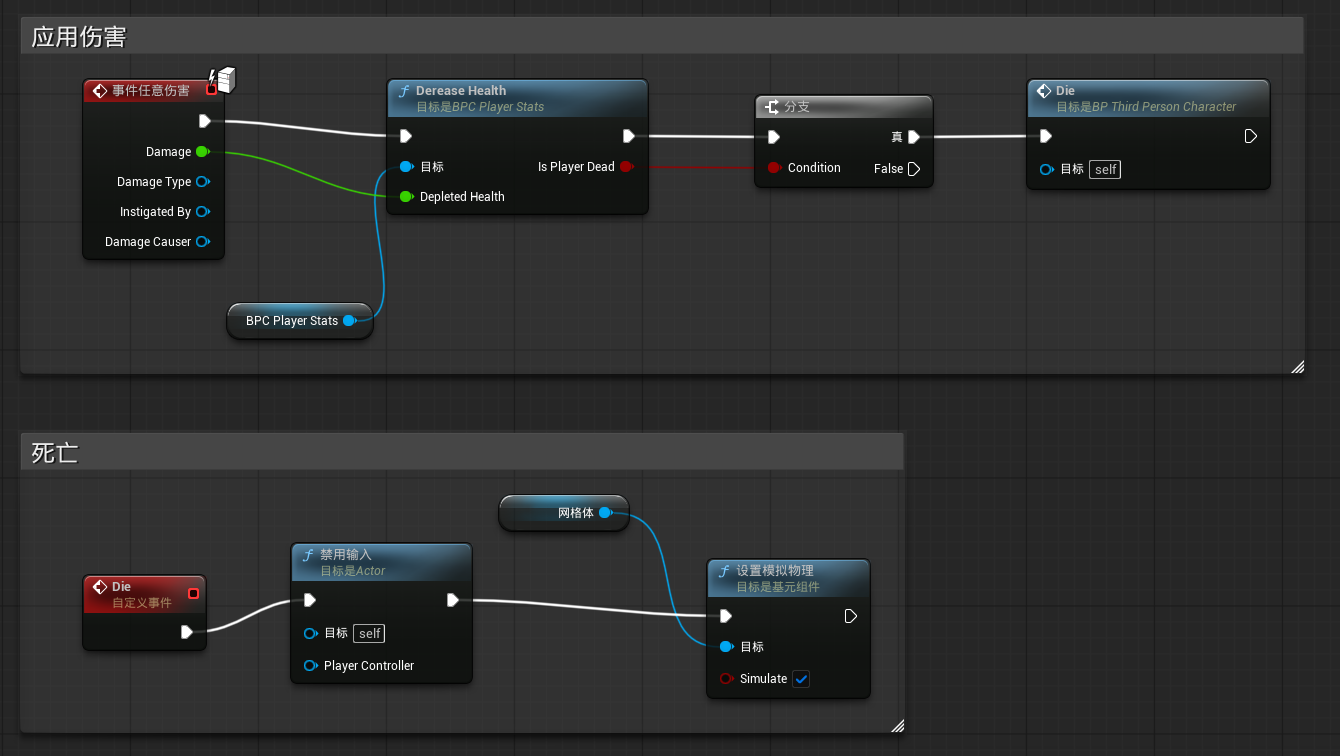
\includegraphics[width=1.0\textwidth]{角色受伤逻辑.png}
\caption{角色受伤逻辑}
\end{figure}

\begin{tip}
    Event tick，逻辑在每一帧都会执行
\end{tip}

\begin{figure}[h]
\centering
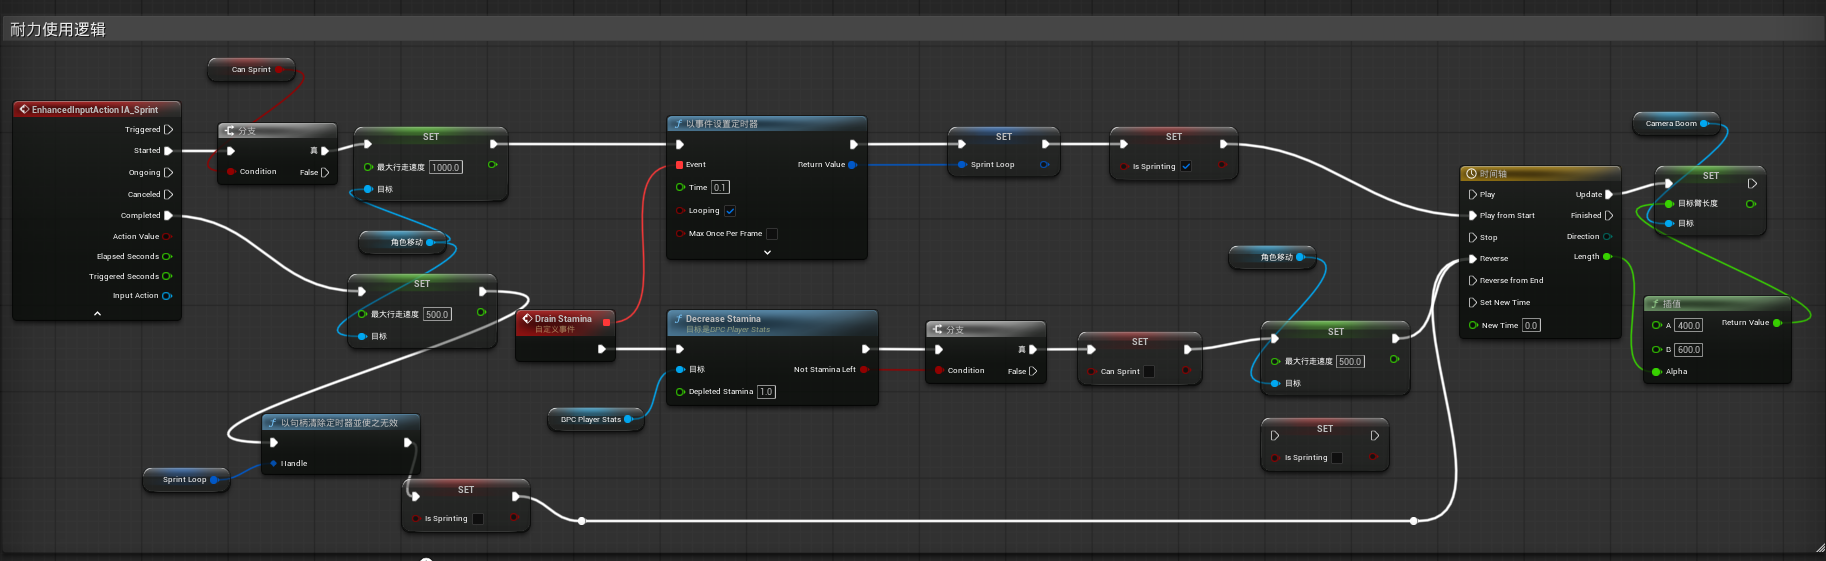
\includegraphics[width=1.0\textwidth]{耐力使用.png}
\caption{耐力使用}
\end{figure}

\begin{figure}[h]
\centering
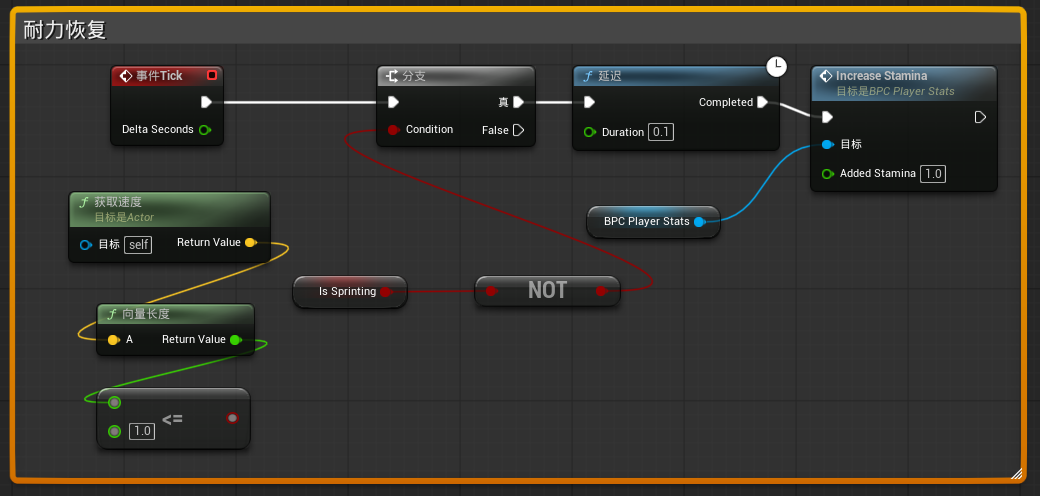
\includegraphics[width=1.0\textwidth]{耐力恢复.png}
\caption{耐力恢复}
\end{figure}


\begin{figure}[h]
\centering
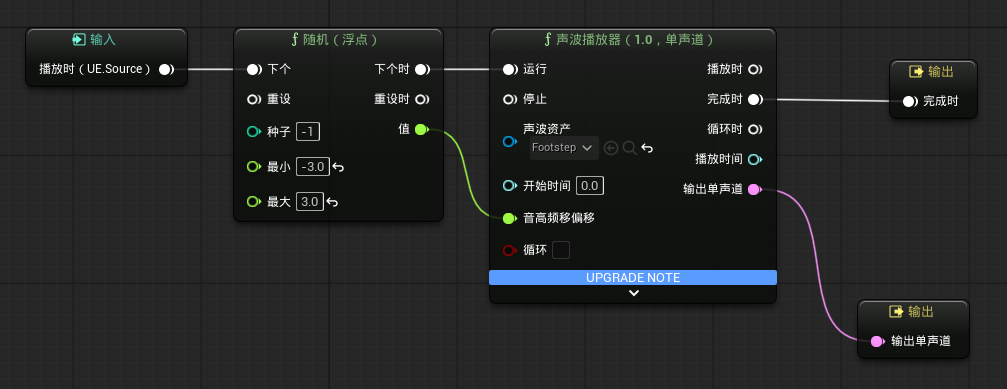
\includegraphics[width=1.0\textwidth]{脚步声.png}
\caption{脚步声}
\end{figure}

\begin{tip}
    设置UI界面时，一定要选择合适的锚点，否则在不同分辨率下UI位置会发生变化
\end{tip}



%---------------------------------------------新章节
\section{战斗系统  }


\begin{itemize}
    \item 新建文件夹SwordAttacks，添加攻击动画，并将所有动画启动根运动。
    \item 新建两个AnimNotify组件，添加函数“接收通知”，用于通知连招的继续和结束。为所有攻击蒙太奇添加这两个通知
    \item 新建BPC\_AttackSystem组件（我们上一个BPC文件用于管理玩家属性），并添加至玩家
    \item 新建攻击动作（鼠标左键）,连招间的切换使用通知实现，
    \item 为了让动画更自然有位移，我们对想实现位移的骨骼树选中root骨骼， 增加若干关键帧，并移动模型位置
    \item 创建剑的材质，右键基础颜色，创建Matiarial，并将各种texture连接（基础颜色，金属度，法线，遮蔽，粗糙度），将材质应用到模型上
    \item 将剑绑定到骨骼上：打开需要绑定的动画，进入骨骼树，选中右手，右键创建插槽Hand\_R\_Sword。对插槽右键单击，添加预览资产，选中剑，并调整位置
    \item 在玩家的静态网格组件中添加静态网格组件，并绑定到剑上，设置剑为无碰撞。
    \item 在动画新建文件夹Hit\_Reacts，添加受击动画，并创建蒙太奇
    \item 在连击系统的基础上增加攻击判定，给剑身加上两个标记（给剑组件增加arrow），将两个端点的坐标传入球形追踪
    \item 增加攻击通知，在播放攻击动画时，激活剑身碰撞的判定逻辑。添加AnimNotifyState->BP\_Notify\_SwordTraceLoop,在通知开始时启动球形追踪，在通知结束时关闭球形追踪，实现逻辑与耐力类似（通过以事件设置定时器）。
    \item 在攻击动画蒙太奇中添加启用攻击判定的通知，该通知用于攻击1和攻击4的判定
    \item 角色攻击2为前刺，攻击3为前踢，我们使用额外的Sphere Trace实现。和前面类似，在角色网格体组件上增加箭头组件，依据箭头位置计算球形检测的起点和终点。由于这个动作比较快，而且只发生一次，我们使用AimNotify实现
    \item 增加伤害逻辑。为假人类默认值中添加新标签“Damageable”，区别该模型是否允许被攻击。该模型受击时，可能和一个动画存在多个碰撞，因此我们使用do once和delay来对应用AimNotifyState的事件控制伤害的频率。对于AimNotify，本身就只执行一次。
    \item 当检测到受击时，对假人应用受到伤害，并在任意伤害发生时，播放受击动画，并接上launch character，施加击退效果
    \item 添加摄像机抖动效果,新建蓝图LegacyCameraShake类BP\_SwordHitCameraShake，并适当调整参数
    \item 为攻击与受击添加音效,使用事件实现，在actor位置播放音效->优化：建立meta sound，让声音更具动态效果
    \item 增加血液特效。在攻击到敌人的逻辑末尾增加粒子发射器Spawn Emitter at Location，选择血液特效,并调整位置与旋转，选择自动释放、
    \item 将玩家属性系统应用到测试假人身上，为测试假人添加新的血量UI（锚点居中）->左上角添加widget并在“用户界面”“控件类”应用刚才的资产
    \item 新建输入“目标锁定”（Tab），以角色为起点，发射射线检测前方物体。若检测到带有“Damageable”标签的物体，则锁定该目标，即在tick事件中实时计算摄像机朝向（F5.24）
    \item 新建动画闪避（Dodge-Roll ），输入“闪避”（X）。注意翻滚的实现中要防止角色重复翻滚且只播放翻滚动画的前几秒->使用蒙太奇而不用动画蒙太奇实现，翻滚播放完成后才允许再次翻滚

\end{itemize}

\begin{figure}[h]
\centering
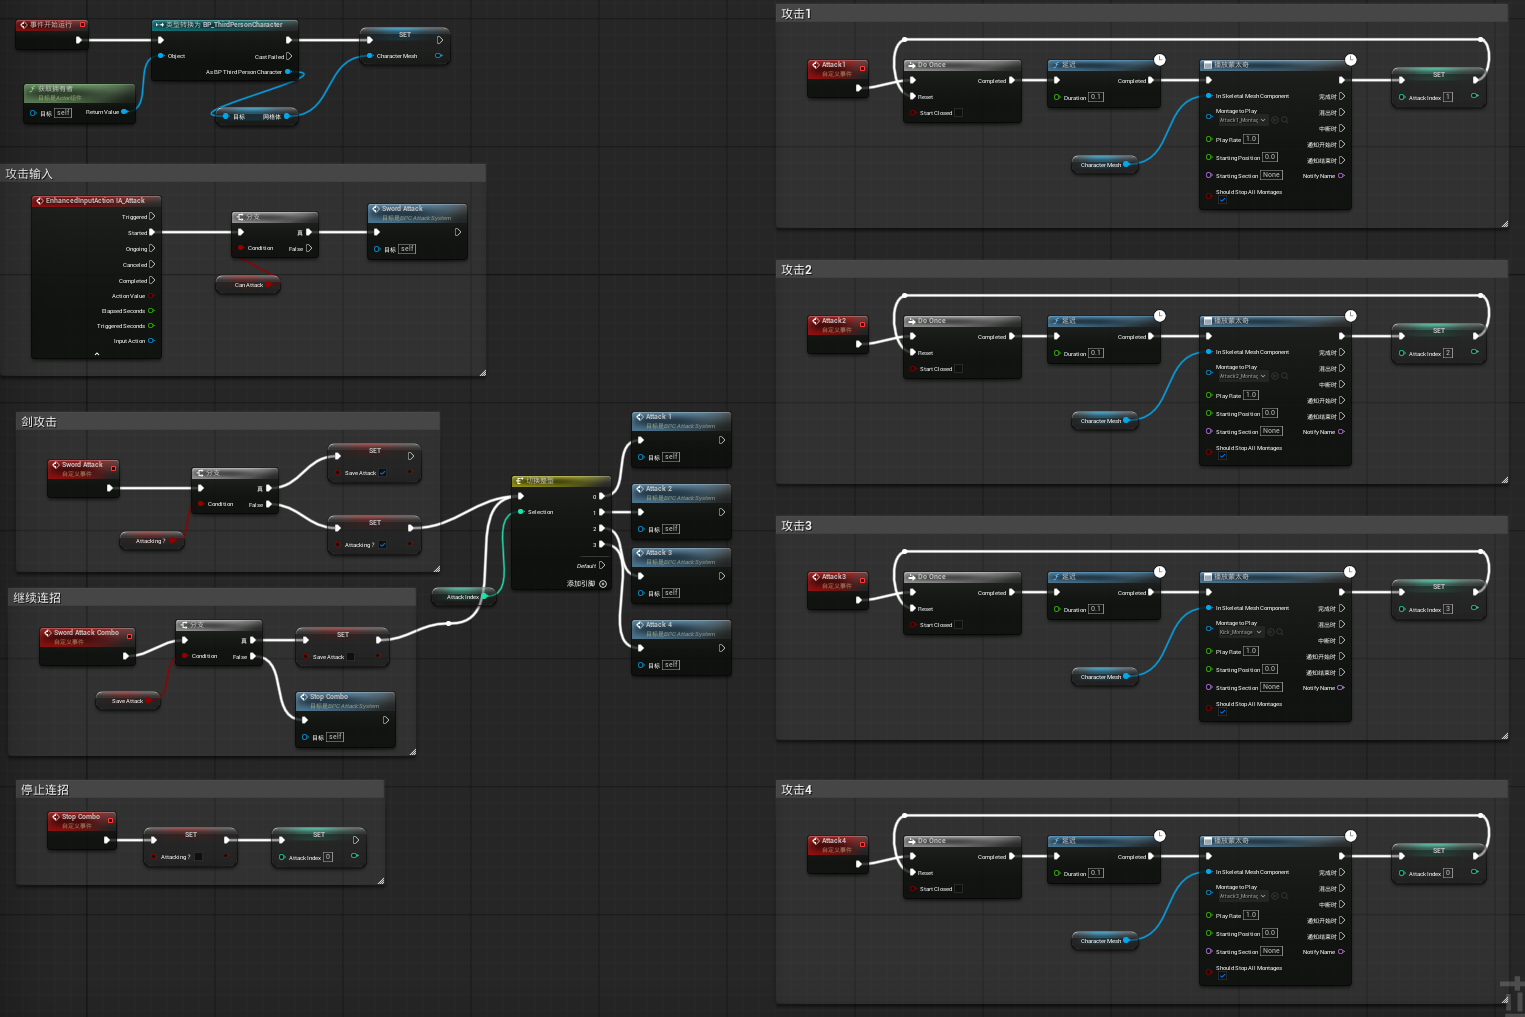
\includegraphics[width=1.0\textwidth]{连招系统.png}
\caption{连招系统}
\end{figure}


\begin{warning}
修复蹲伏拉视角反向播放逻辑，使得快速按两次ctrl时，视角不会卡到结尾

\end{warning}

\begin{tip}
AimNotify通知仅仅能接收信号什么时候开始，我们用于连招。在连招期间，一旦收到信号则继续连招；
AimNotifyState可以区分信号的开始和结束，我们用于攻击判定，仅仅在攻击的时候启用碰撞判定

\end{tip}


\begin{tip}
在地图中选择物体，按ctrl+e可以快速打开它的面板
\end{tip}


\begin{tip}
可建立动画蒙太奇类变量，使用数组，实现不同动画的随机播放
\end{tip}

\begin{figure}[h]
\centering
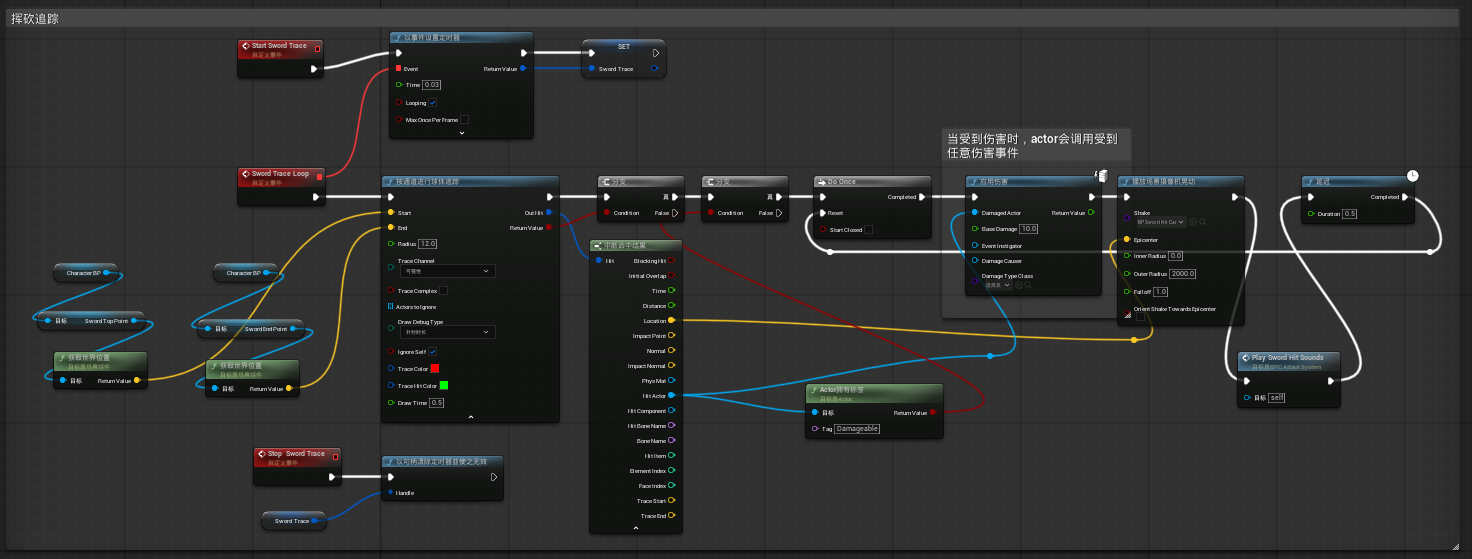
\includegraphics[width=1.0\textwidth]{挥砍追踪.png}
\caption{挥砍追踪}
\end{figure}

\begin{figure}[h]
\centering
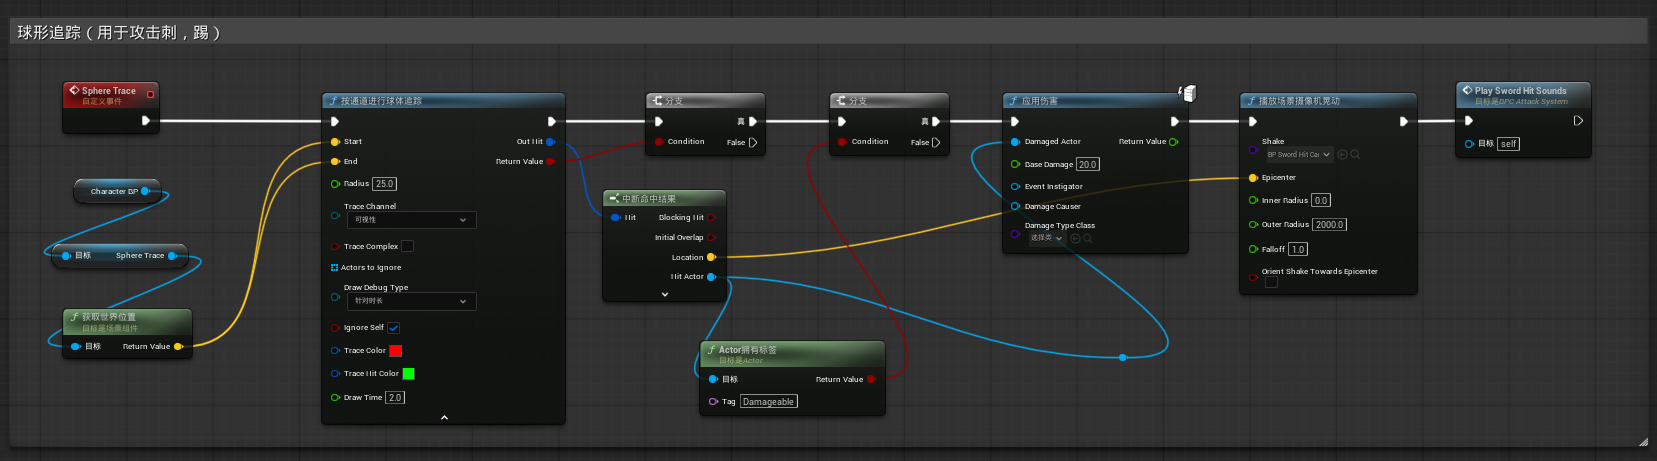
\includegraphics[width=1.0\textwidth]{球形追踪.png}
\caption{球形追踪}
\end{figure}

\begin{figure}[h]
\centering
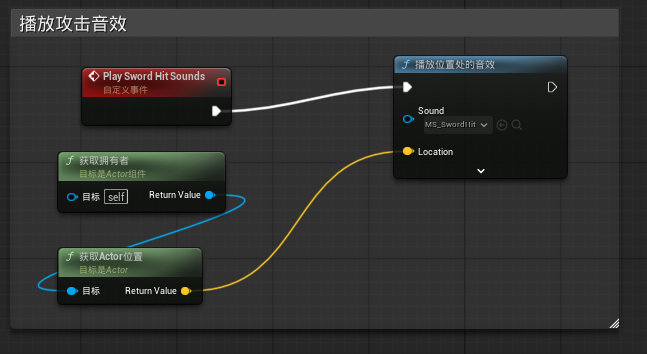
\includegraphics[width=1.0\textwidth]{挥砍音效.png}
\caption{挥砍音效}
\end{figure}


\begin{warning}
    当我们想把属性系统应用到假人身上时，由于我们之前写的所有逻辑都基于第三人称角色，因此原来的逻辑将无法获取到对象
    -> 在原来的cast to第三人称角色组件上的cast failed节点接入额外的处理分支，设置isPlayer标志系统当前的拥有者是谁
\end{warning}



\begin{tip}
将widget“细节”中，“用户界面”“空间”改为屏幕，则玩家在任何位置都能看到该UI面对玩家
\end{tip}

\begin{figure}[h]
\centering
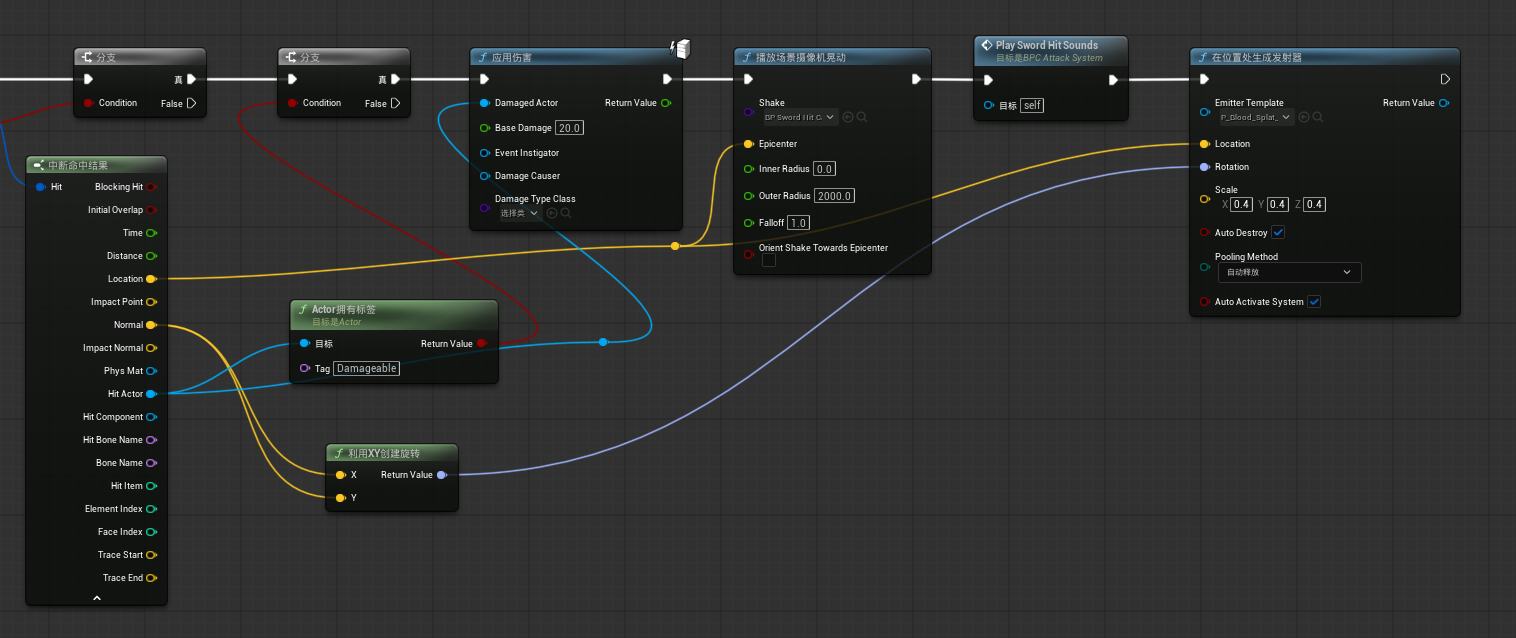
\includegraphics[width=1.0\textwidth]{血液粒子特效应用.png}
\caption{血液粒子特效应用}
\end{figure}

\begin{figure}[h]
\centering
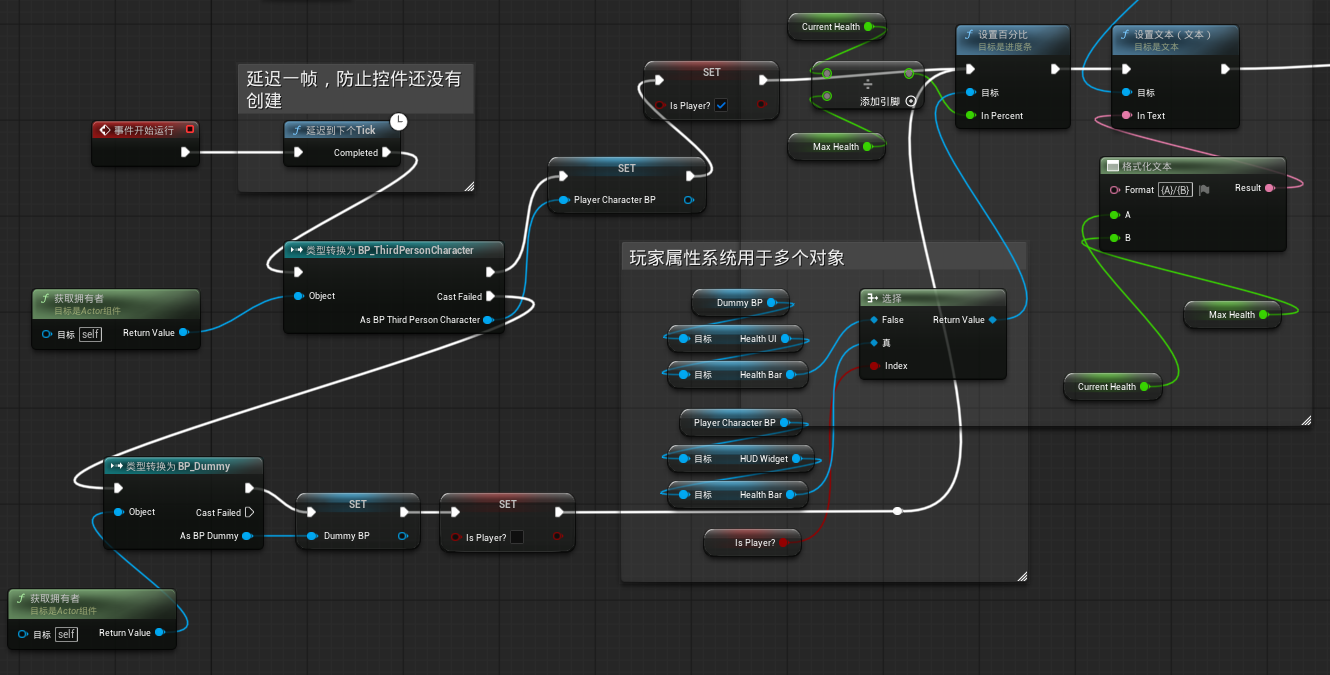
\includegraphics[width=1.0\textwidth]{属性刷新UI逻辑更新.png}
\caption{属性刷新UI逻辑更新}
\end{figure}


\begin{warning}
假人被杀死后，模型虽然变为了布娃娃，但是碰撞体还在，我们仍然可以攻击到虚空中的假人碰撞体，并令之发出呻吟 -> 等待后续修复
\end{warning}

\begin{warning}
角色蹲伏以后，胶囊体并没有随之减小，因此无法穿过狭小的空间 -> 在蹲伏逻辑中，调整胶囊体的半高 -> 90 到 60，然而这样会导致角色的中心点发生变化，出现卡住的情况 -> 调整角色模型的Z高度，加上30的偏移量
\end{warning}

\begin{tip}
可以通过设置相机的启用摄像机延迟，来改变相机跟随玩家移动的速度，从而使移动更平滑
\end{tip}

\begin{tip}
可以通过sequence组件实现并行操作
\end{tip}

\begin{figure}[h]
\centering
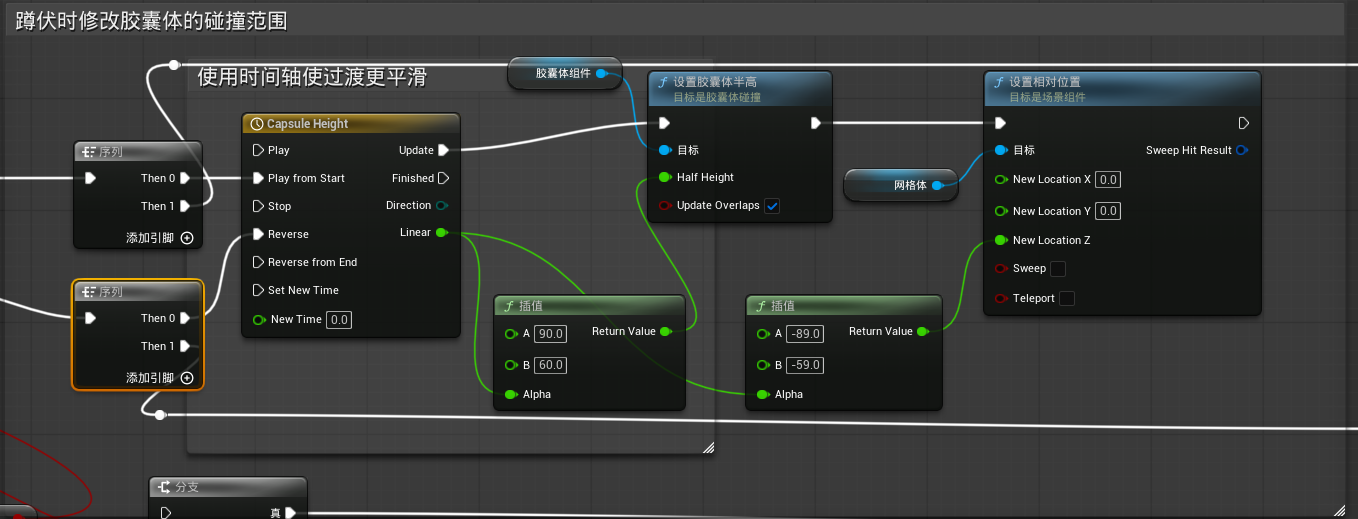
\includegraphics[width=1.0\textwidth]{设置胶囊体半高.png}
\caption{设置胶囊体半高}
\end{figure}

\begin{figure}[h]
\centering
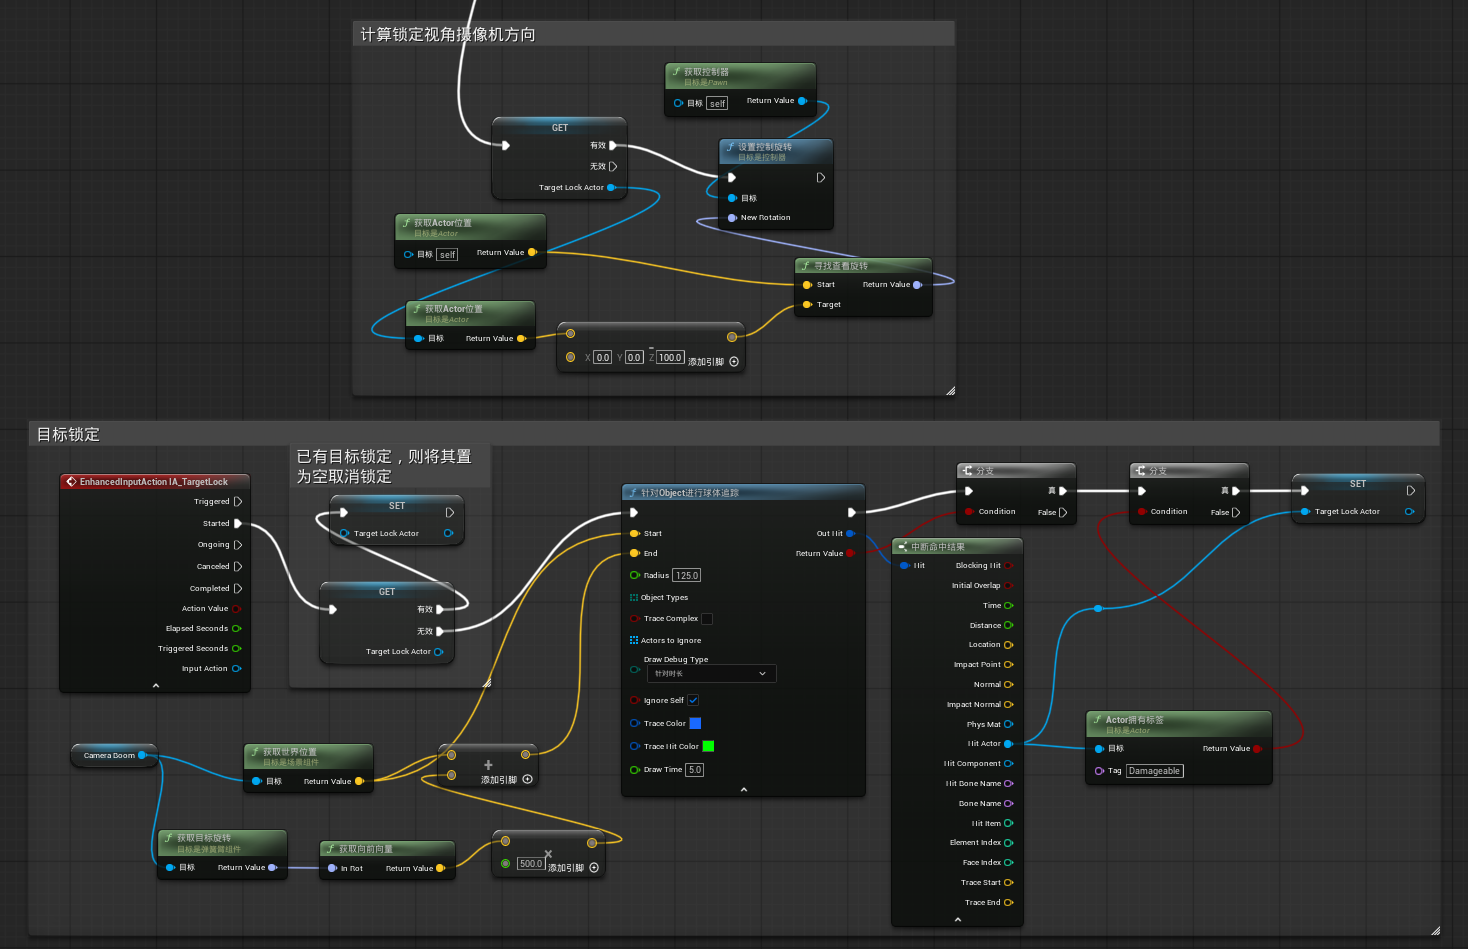
\includegraphics[width=1.0\textwidth]{目标锁定.png}
\caption{目标锁定}
\end{figure}

\begin{tip}
Play Montage与Play Aim Motagehic的区别：前者端口更多，可以用于判定动画是否完成；后者只是播放动画
\end{tip}

\begin{warning}
目标锁定时，球形通道总是检测所有物体，并且在第一个接触点中断，导致我们的目标锁定总是碰到地面从而失效 -> 将按通道进行球形追踪改为按object进行球形追踪，并且勾选物理形体
\end{warning}


\begin{figure}[h]
\centering
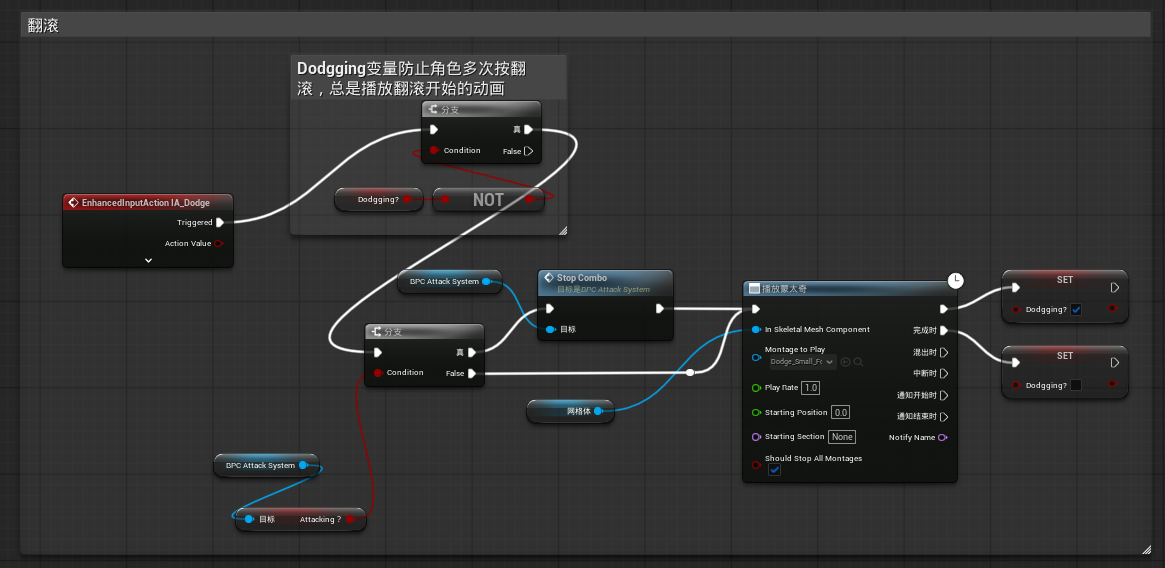
\includegraphics[width=1.0\textwidth]{翻滚.png}
\caption{翻滚}
\end{figure}


\begin{warning}
翻越时，假设物体非常高，我们依然能计算出有效的碰撞起点，碰撞中点以及着陆点，导致角色从物体中间飞过去 -> 增加检测中点穿过某个物体的逻辑（F5.26），若最终计算的中点和物体发生了重叠，则不允许翻越
\end{warning}

\begin{figure}[h]
\centering
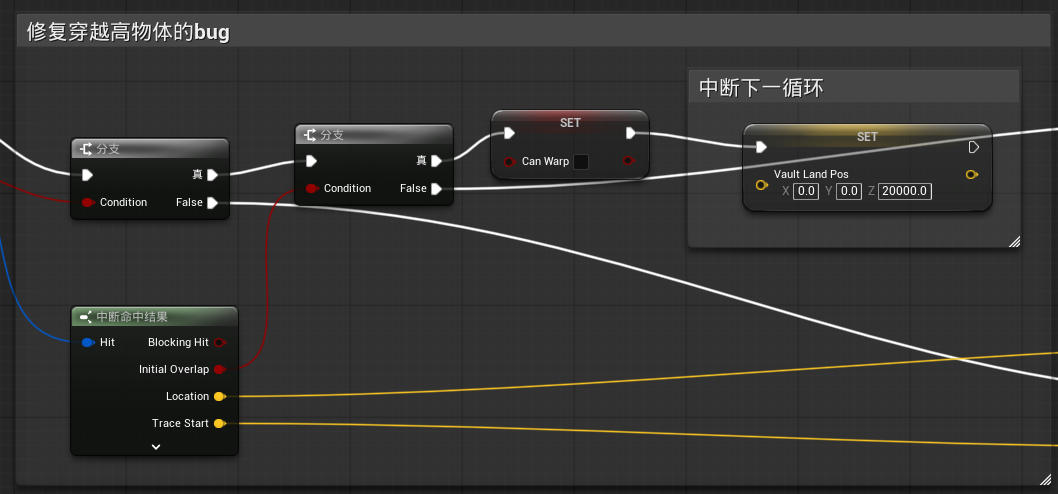
\includegraphics[width=1.0\textwidth]{修复翻越逻辑.png}
\caption{修复翻越逻辑}
\end{figure}



%---------------------------------------------新章节
\section{装备系统} 

\begin{itemize}
    \item 新建文件夹 Equipment\_System，保存装备系统的资源
    \item 新建“蓝图”“结构” S\_Weapons，用于保存手持物品的参数，包括名称，伤害，等级，图标，静态网格体，类型（枚举器），武器槽位;“结构” S\_Slots,包含一个"数据表行处理"类型的物品(item)
    \item 新建“蓝图”“枚举”E\_Weapon\_Types，用于保存所有的武器类型：近战武器，远程武器，盔甲，盾牌
    \item 新建“其他”“数据表格” DB\_Weapons,行结构体选择我们之前创建的结构S\_Weapons，在里面添加武器实例的信息。
    \item 新建“Actor” BP\_Weapon，用于放置在场景中可被玩家拾取的武器。新建S\_Slots类型的变量itemData,并打开“可编辑实例”“生成时公开”。在构造脚本中为该蓝图选择静态网格体。
    \item 新建“Actor Component” BPC\_EquipmentSystem，管理武器相关的属性。新建函数添加武器。
    \item 添加输入操作IA\_Interact(F),按下后在周围进行球形追踪，检测是否有武器实例，如果有则调用添加武器函数，并销毁武器实例
    \item 新建UI文件夹，用于装备系统的UI显示。添加输入操作IA\_EquipmentMenu(M)，按下后打开背包,显示鼠标光标并启用ui输入，同时设置移动模式为空。关闭背包后需要恢复
    \item 使用Widget添加装备槽的UI，并将其放置在装备UI中的垂直框当中。单击装备槽，可以弹出一个新UI，显示背包中所有武器的列表，再点击屏幕任意位置，令控件不可见
    \item 允许选择装备列表中的装备，装备列表项新建按钮，在普通状态下，更改其着色不透明度为0，悬停时加入一点透明度。
    
    \item 在装备UI中间添加玩家视口。在角色视口新建弹簧臂，调整角度使其正对玩家，取消勾选“进行碰撞测试”；在上面添加场景捕获2D组件,该组件能将捕获到的图像保存为纹理，“基元渲染模式”->"使用仅显示列表"，并将角色添加入列表。
    \item 场景捕获器中“场景捕获”“纹理目标”新建“渲染目标”至装备文件夹，将“渲染纹理目标2D”的尺寸改为2048*2048,并右键“创建材质”遮罩捕获的天空盒。给装备UI中间的图片“笔刷”“图像”选择该材质
    \item 虽然完成了显示，但是中间这个角色很小，还被拉伸了-> 增加缩放框，限制按比例拉伸，将图像放入缩放框中。并且给UI加了背景和背景模糊
    \item 给装备列表项添加点击逻辑。新建变量CurrentEquipableSlot，保存当前正在点击的装备槽。给每个列表项新建S\_Slots型变量，保存这个列表项自己对应的武器数据行。在创建列表项时写入。
    
    \item 增加装备武器函数，获取装备槽中的S\_Slots内容，改变当前武器的静态网格体模型（F5.34）。
    \item 对装备槽进行分类，给装备槽添加新变量slotCategory，表示该槽允许装备的物品，并点击小眼睛将其设置为公共变量。每个槽只打开该类别下的列表项
    \item 增加盾牌与弓箭装备以及它们的正确槽位（都Spine5上创建插槽），在Assign Slot时，在枚举类型上switch，进入不同的处理逻辑（F5.35）,不同逻辑的差别仅仅是操作角色不同位置的静态网格体组件

\end{itemize}

\begin{figure}[h]
\centering
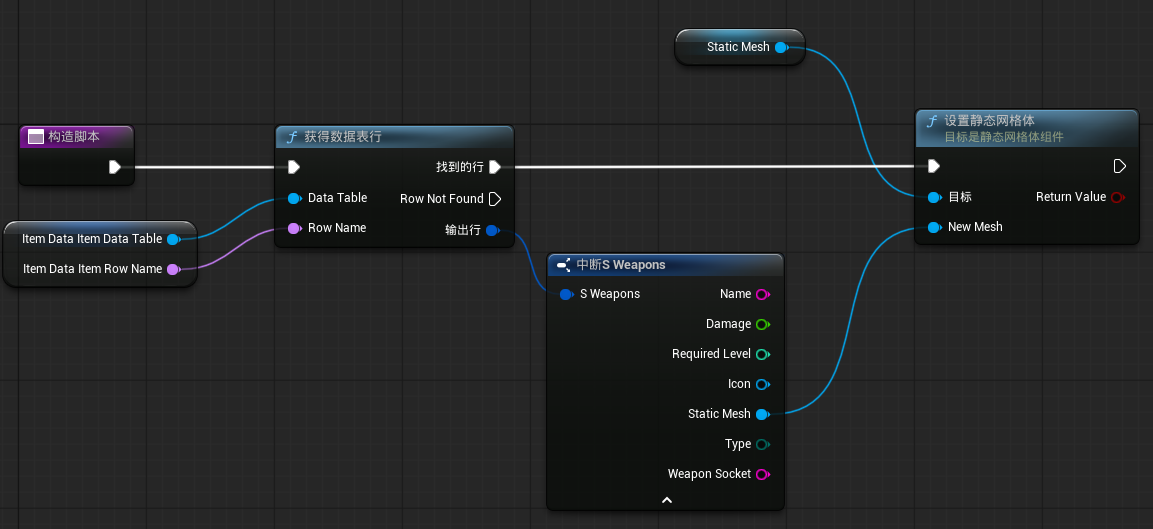
\includegraphics[width=1.0\textwidth]{设置可编辑实例武器的网格体.png}
\caption{设置可编辑实例武器的网格体}
\end{figure}


\begin{figure}[h]
\centering
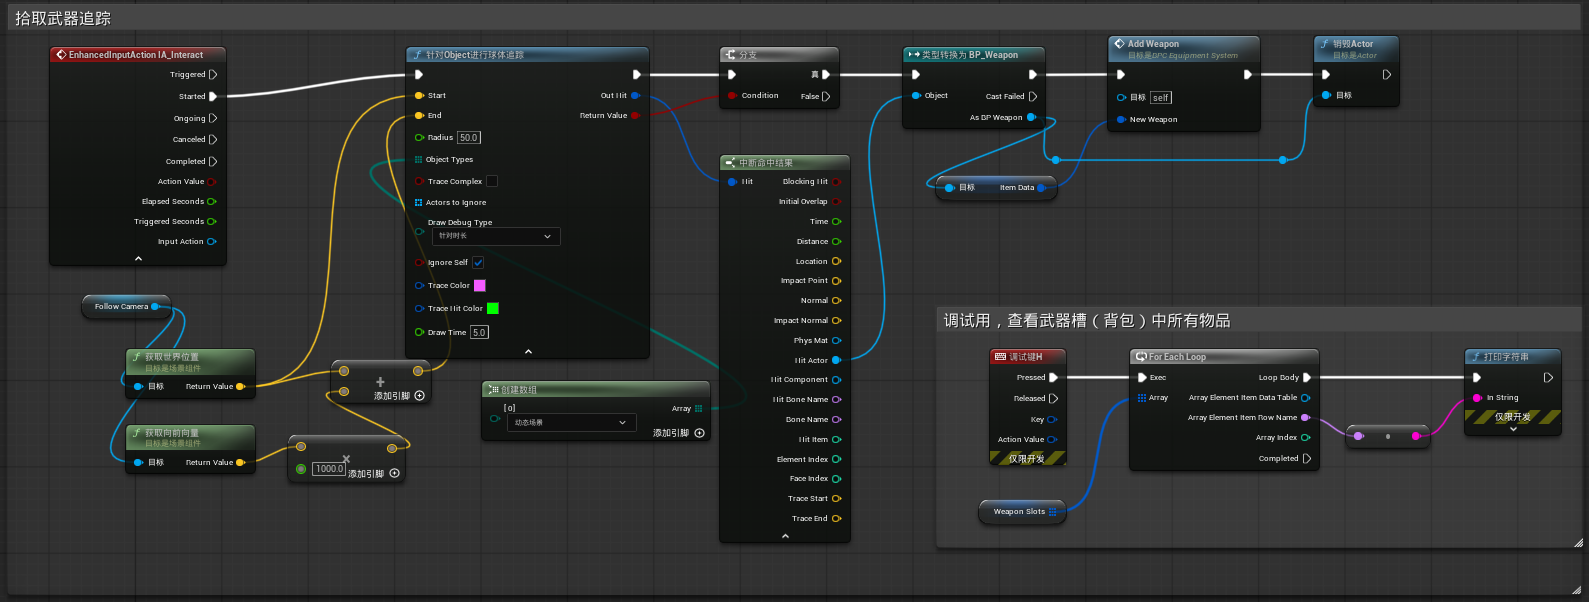
\includegraphics[width=1.0\textwidth]{拾取武器追踪.png}
\caption{拾取武器追踪}
\end{figure}

\begin{warning}
在打开装备UI面板时，我们要允许输入模式接收UI和游戏输入，否则按M键回不去了
\end{warning}

\begin{figure}[h]
\centering
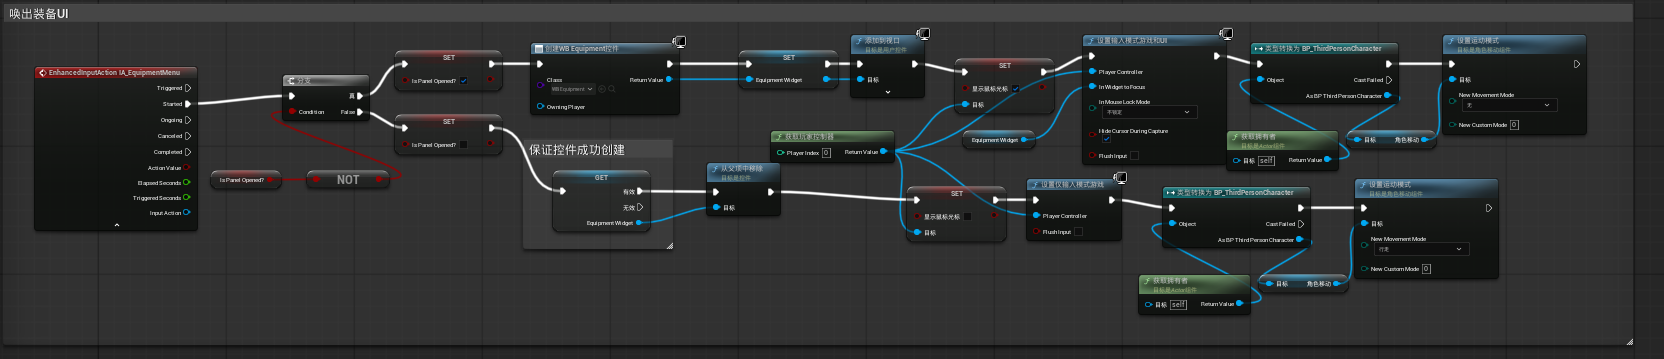
\includegraphics[width=1.0\textwidth]{背包UI.png}
\caption{唤出与关闭背包UI}
\end{figure}

\begin{figure}[h]
\centering
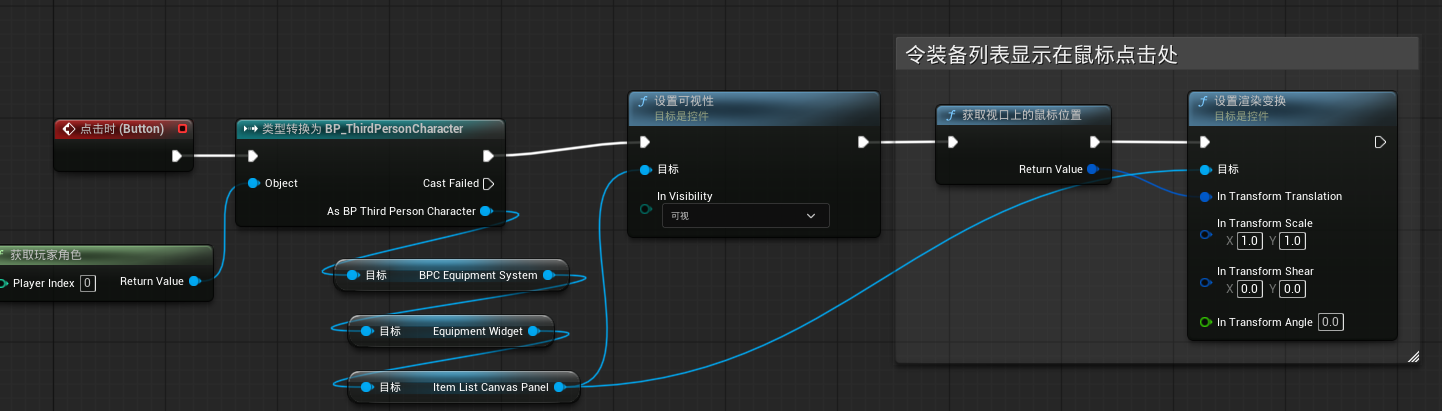
\includegraphics[width=1.0\textwidth]{装备列表.png}
\caption{按装备槽按钮显示装备列表}
\end{figure}


\begin{warning}
需要留意widget布局中的先后顺序，下面的组件会覆盖上面的组件！
\end{warning}

\begin{figure}[h]
\centering
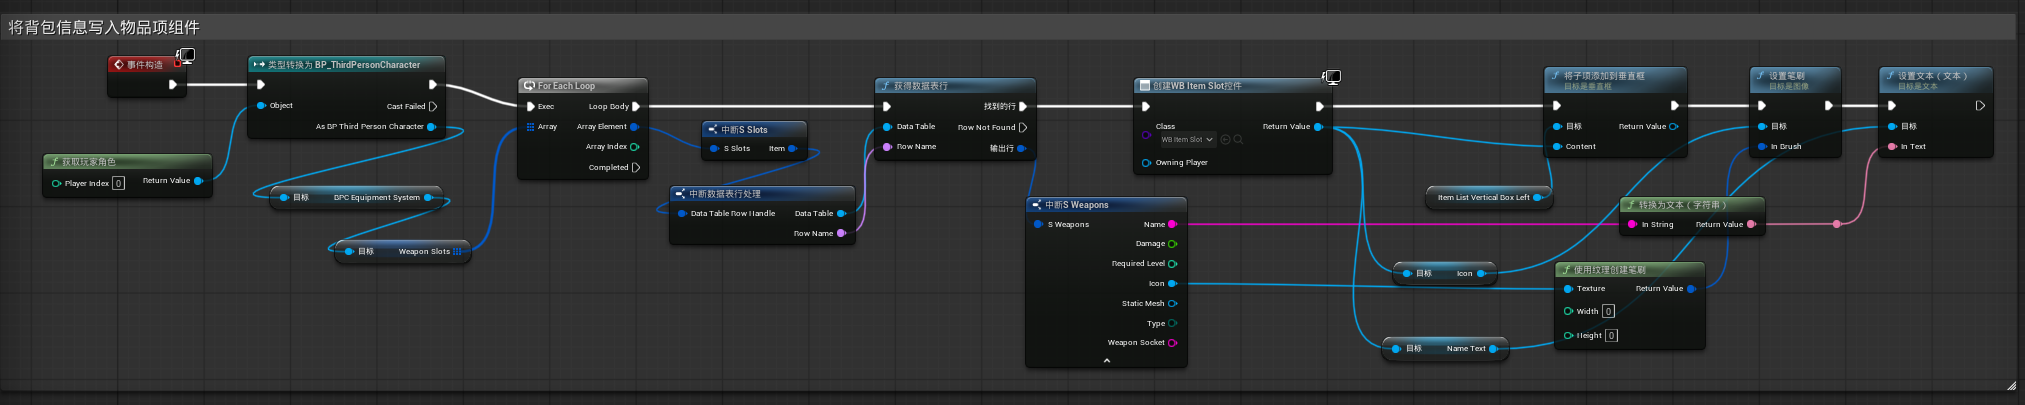
\includegraphics[width=1.0\textwidth]{将背包中物品信息写入物品项.png}
\caption{将背包中物品信息写入物品项}
\end{figure}

\begin{figure}[h]
\centering
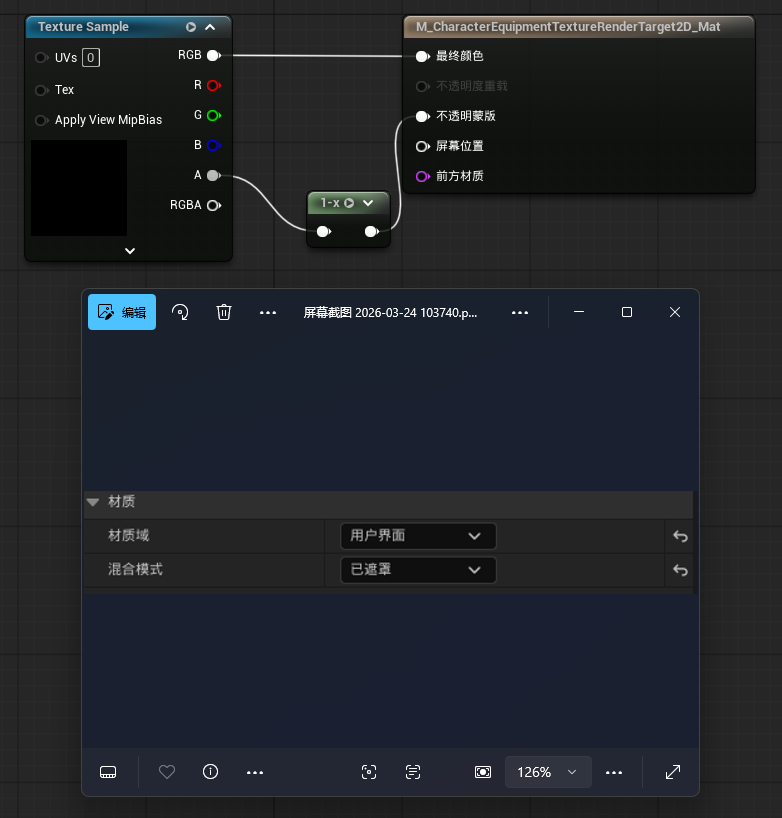
\includegraphics[width=1.0\textwidth]{遮罩场景捕获天空.png}
\caption{遮罩场景捕获天空材质设置}
\end{figure}

\begin{figure}[h]
\centering
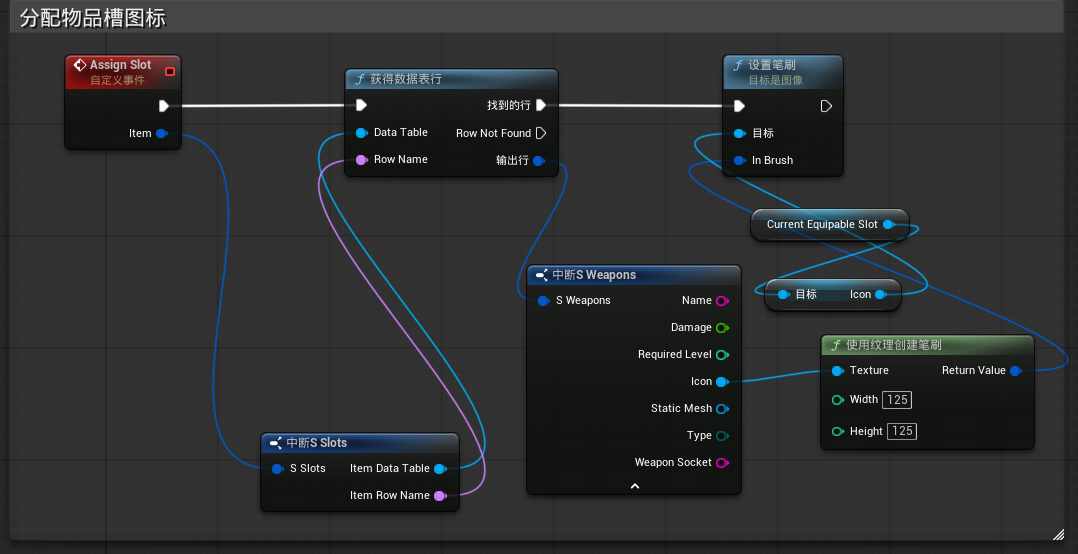
\includegraphics[width=1.0\textwidth]{分配物品槽图标.png}
\caption{分配物品槽图标}
\end{figure}


\begin{figure}[h]
\centering
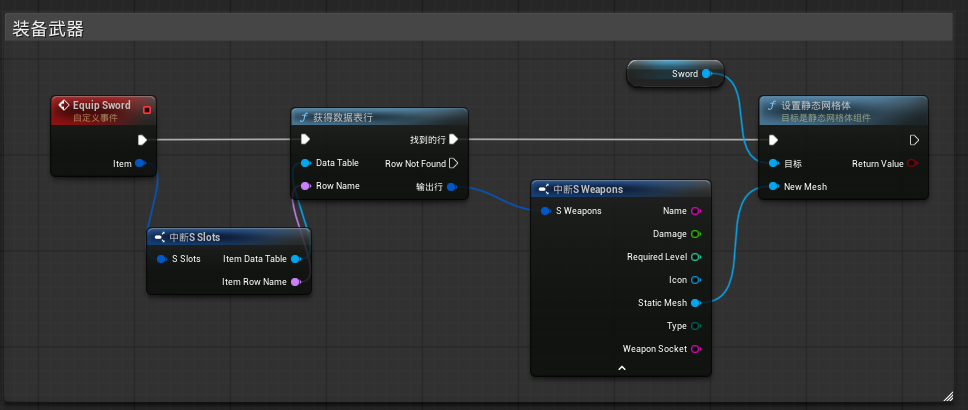
\includegraphics[width=1.0\textwidth]{装备武器.png}
\caption{装备武器}
\end{figure}

\begin{warning}
装备武器列表项越来越多 -> 每次生成列表项时，都要清除之前生成的项，重新生成列表项
\end{warning}


\begin{warning}
当我们打开背包装备武器再关闭，然后再打开时，由于生成的是另外的widget实例，所以之前的武器装备图标消失了 ->
在关闭窗口时不再将其被父级移除并置空，而是隐藏起来;在打开窗口时，若是已生成，则设置可见，否则才创建
\end{warning}


\begin{warning}
我们没有装备剑时，由于攻击动作绑定在角色身上，所以仍然可以播放攻击动画且执行碰撞判定。
-> 在begin play时，如果sword mesh组件没有被赋值，设置攻击系统can attack为false。
\end{warning}


\begin{figure}[h]
\centering
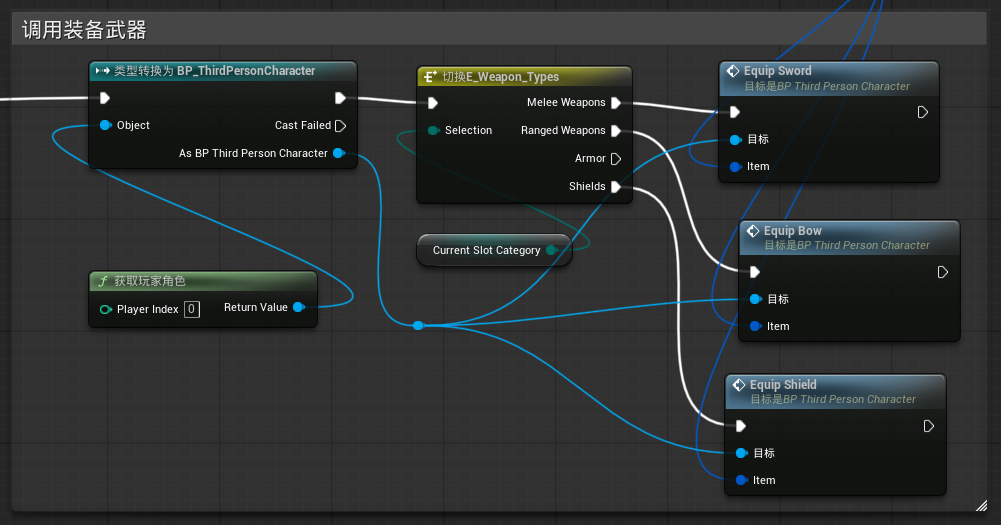
\includegraphics[width=1.0\textwidth]{装备不同类型的武器.png}
\caption{装备不同类型的武器}
\end{figure}

装备系统补充,拾取护甲：
\begin{itemize}
    \item 对新导入的装备，使用“建模模式”，在xForm中编辑轴枢点，改为“中央”
    \item 为模型人的骨骼创建不同的插槽:头盔->head，颈部装甲 -> neck01, 肩甲 ->spine05,胸甲 -> spine05 .....
    \item 给模型网格体添加想要的组件，选择插槽，并禁用碰撞
    \item 在数据库中添加盔甲的相关信息，由于一套盔甲使用了大量的插槽，所以在数据库中我们不设置默认插槽。
    \item 给所有的盔甲设计相同的tag“Bronze Armor”，并默认为不可见。装备时检索名称，
\end{itemize}

\begin{figure}[h]
\centering
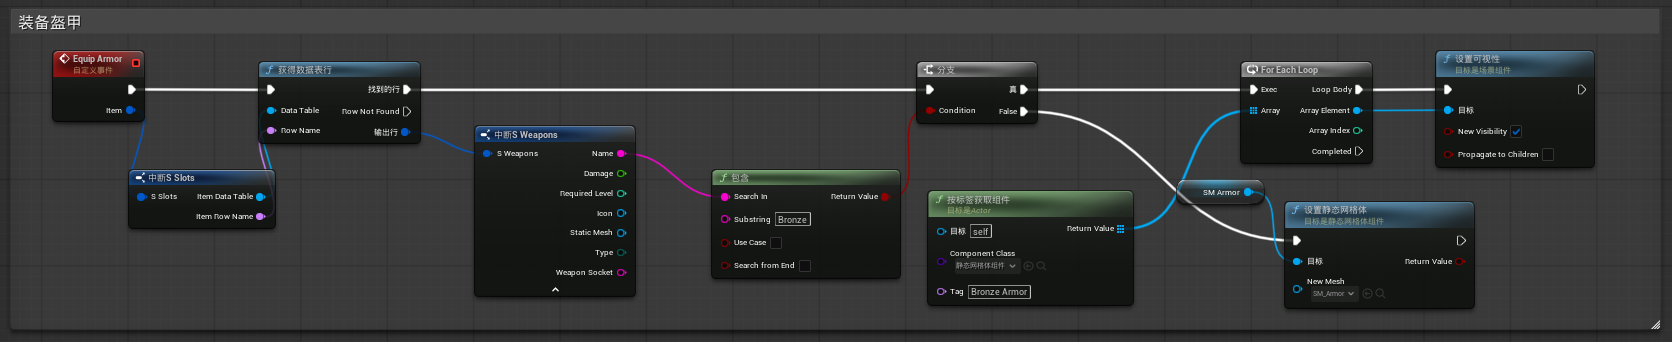
\includegraphics[width=1.0\textwidth]{装备盔甲.png}
\caption{装备盔甲}
\end{figure}


%---------------------------------------------新章节
\section{攀爬移动} 

攀爬：
\begin{itemize}
    \item 在第三人称角色蓝图中，启用角色“移动能力”“可飞行”，复用角色的飞行系统来构建攀爬系统
    \item 新建输入映射“攀爬”（Q），创建新函数用于表面附着计算（F5.36）  
    \item 修改IA\_Move组件，按移动模式进行选择，并将攀爬模式的y输入用于向上移动（F5.37），其中攀爬移动为(F5.38)
    \item 实现停止攀爬函数（F5.39）：当角色不再检测到可攀爬的表面，或再次按下攀爬键（F5.38）
    \item 实现攀爬动画
    \subitem 创造包含四个方向运动的混合空间，使用水平轴和垂直轴。在状态机中增加状态“Climbing” ，可与Locomotion相互转换，条件依赖于一个变量isClimbing。其中向下攀爬动画可用向上攀爬动画速率*-1实现
    \subitem 在ABP事件图中设置我们需要的水平和垂直速度以及isClimbing，前两者需要在角色蓝图中创建对应变量，在我们Move的时候获取（修改F5.37）,ABP事件图设置（F5.40）
    \subitem bug：攀爬时角色无输入仍在动->当速度小于1时，将水平和垂直速度置为0（F5.41）
    \subitem bug:攀爬停止时，有一定概率角色模型飞离碰撞体-> 脚步IK造成 -> 增加启用IK时检测isClimbing
    \subitem bug:攀爬时各动画之间存在偏移 -> 统一各个动画的起始帧的根骨格Z坐标（添加关键帧）。穿模问题同样设置根骨骼起始帧的坐标实现
\end{itemize}

\begin{figure}[h]
\centering
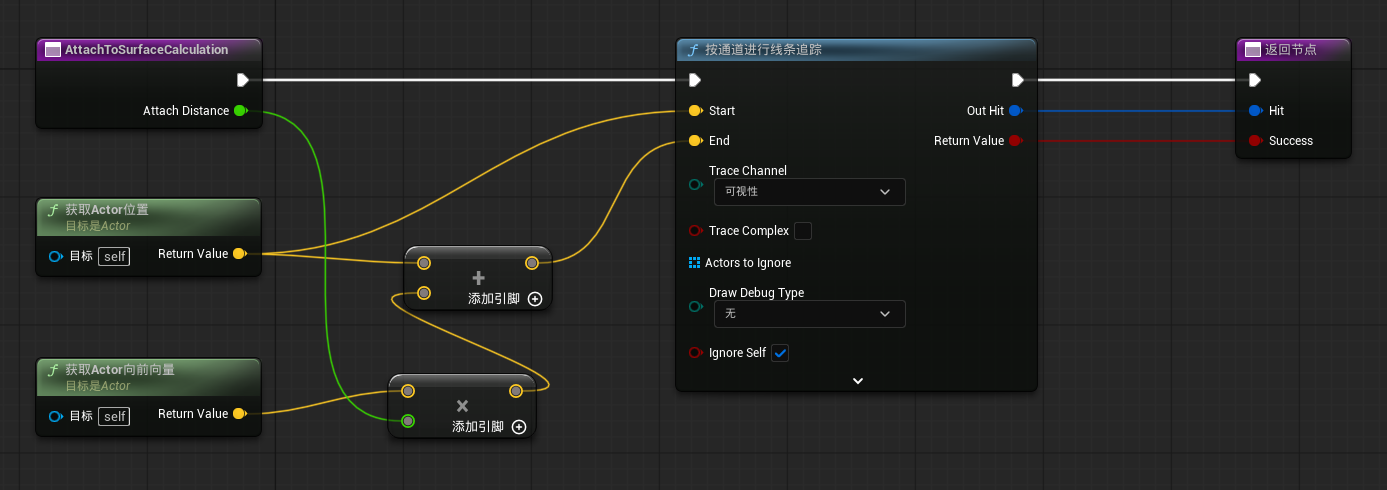
\includegraphics[width=1.0\textwidth]{计算表面附着.png}
\caption{计算表面附着}
\end{figure}

\begin{figure}[h]
\centering
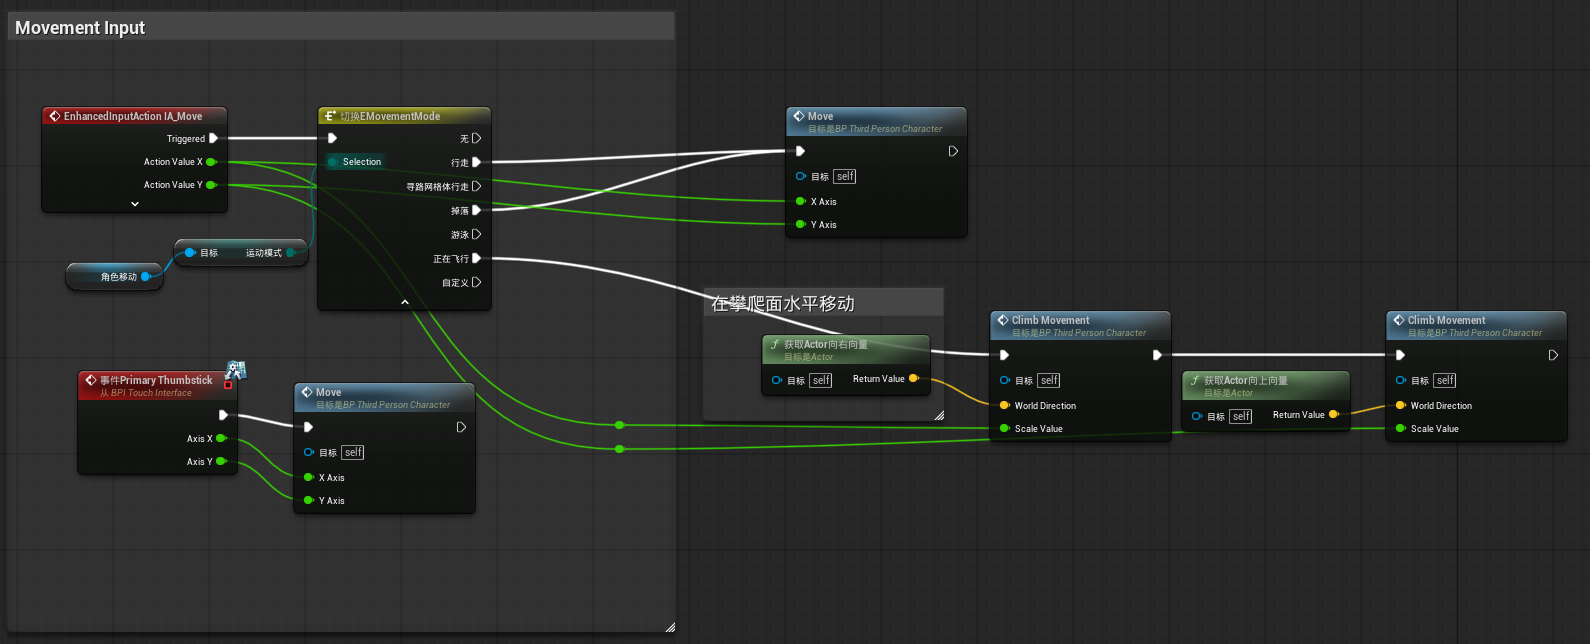
\includegraphics[width=1.0\textwidth]{修改移动输入.png}
\caption{修改移动输入}
\end{figure}

\begin{figure}[h]
\centering
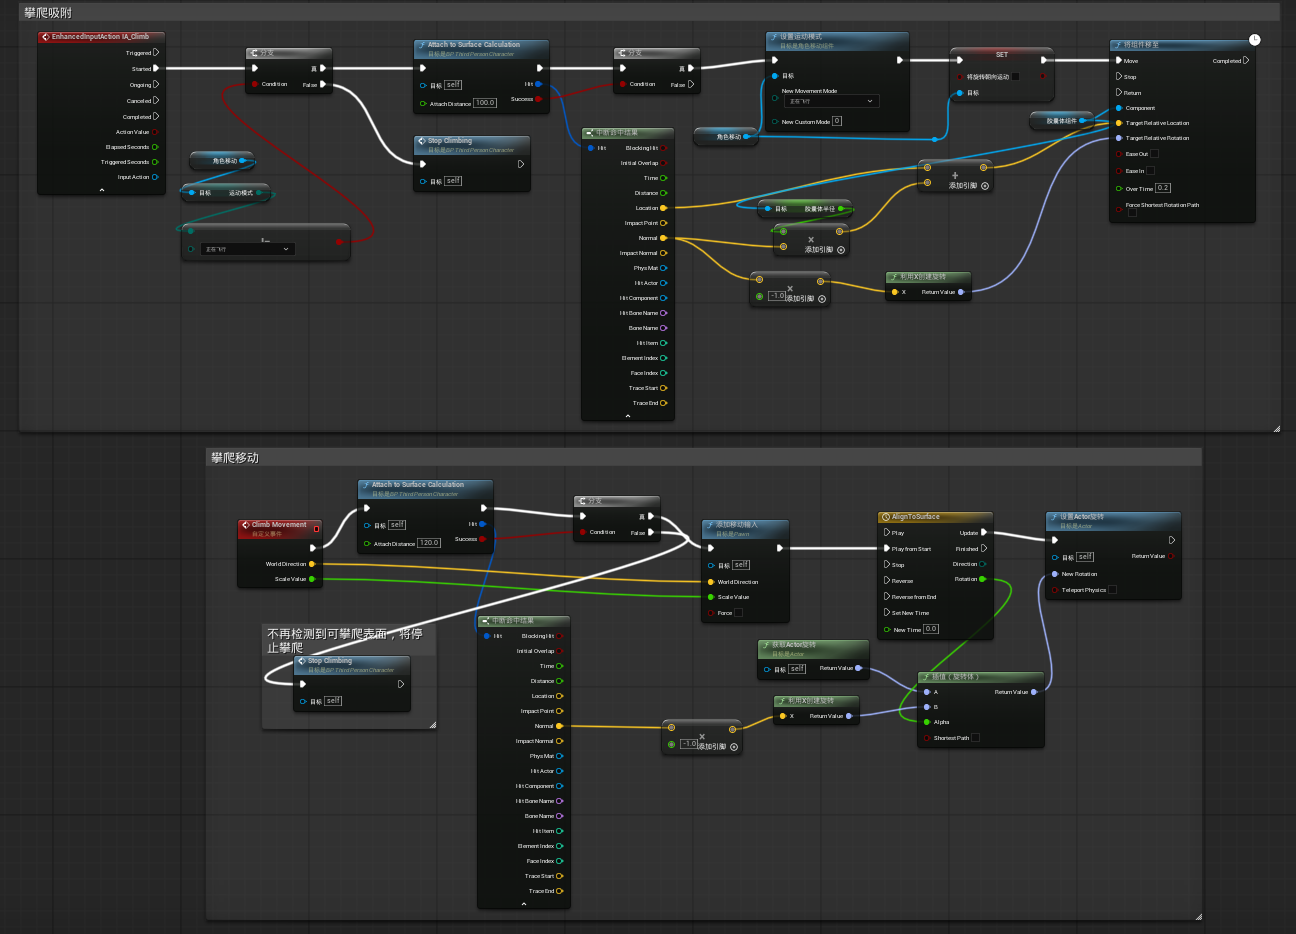
\includegraphics[width=1.0\textwidth]{攀爬移动.png}
\caption{攀爬移动}
\end{figure}

\begin{figure}[h]
\centering
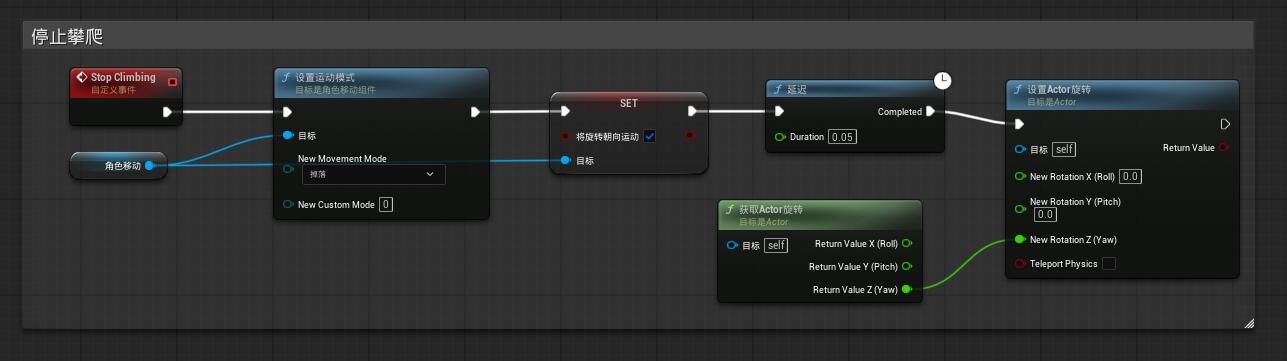
\includegraphics[width=1.0\textwidth]{停止攀爬.png}
\caption{停止攀爬}
\end{figure}


\begin{figure}[h]
\centering
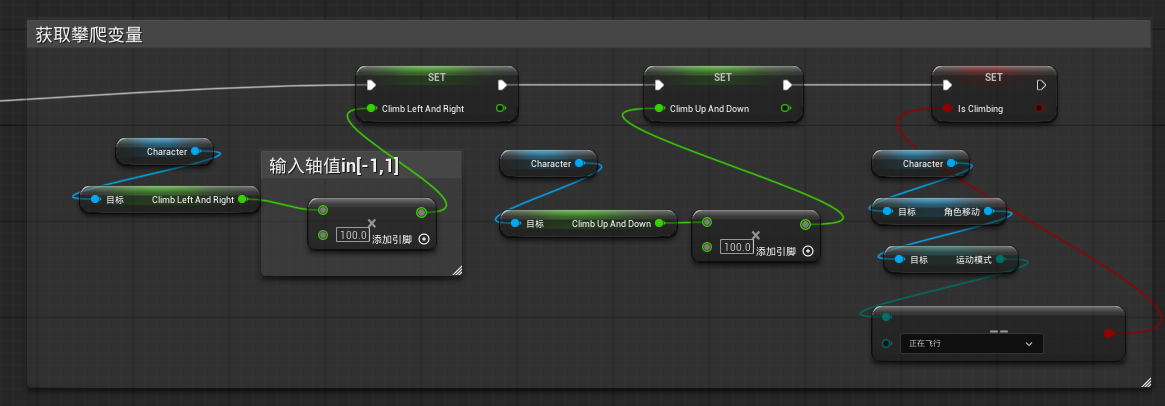
\includegraphics[width=1.0\textwidth]{获取攀爬变量.png}
\caption{获取攀爬变量}
\end{figure}


\begin{figure}[h]
\centering
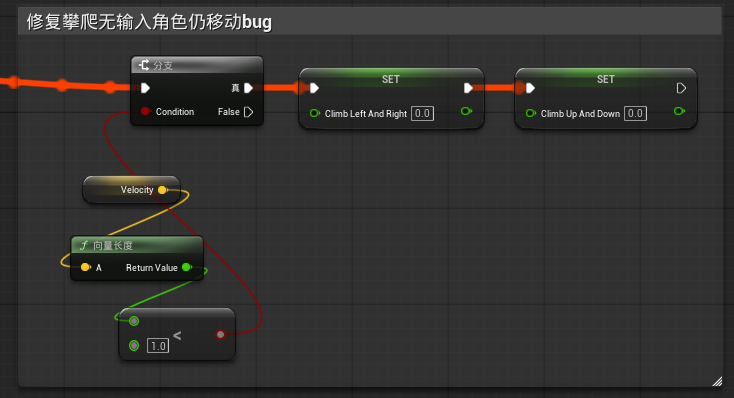
\includegraphics[width=1.0\textwidth]{修复攀爬bug.png}
\caption{修复攀爬bug}
\end{figure}

抓边攀爬：
\begin{itemize}
    \item 对抓边攀爬动作启用根骨格运动
    \item 在角色中实现检测边缘逻辑（在角色头顶向前方发出射线检测），在攀爬移动中旋转actor正对平面法线之前应用
    \item 检测头顶边缘首先在头顶位置朝面对的方向发出射线检测，一旦检测不到命中，说明头顶到达了边缘，此时进行竖直方向上的射线检测，首个命中点就是我们进行运动扭曲的目标位置。（F5.42-5.44）
    \item 创建蒙太奇，其中设置两个运动扭曲通知点，一个是我们向上运动时，一个是攀爬上去以后向前移动。否则角色会沿直线直接穿模到目标位置。最后设置一个蒙太奇通知，用于设置角色在攀爬过程中禁用碰撞检测
    \item 在第三人称角色中使用motion warp组件实现通信：“更新扭曲目标”，名字必须完全一样
\end{itemize}

\begin{warning}
由于攀爬目前设置的模式是飞行模式，与我们翻越时的运动模式一致，所以目前翻越动画完成后，会错误的显示一下攀爬动作
->目前只要是飞行模式角色就会执行攀爬动画 -> 修改is climbing的判断逻辑（F5.40），加入条件没有在is warping

\end{warning}

\begin{figure}[h]
\centering
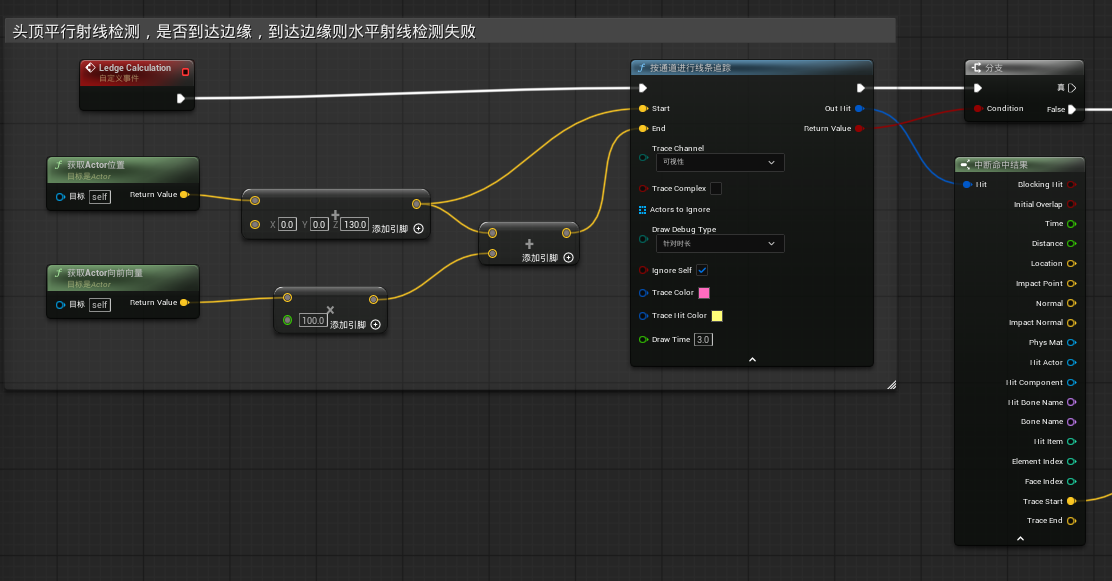
\includegraphics[width=1.0\textwidth]{抓边攀爬1.png}
\caption{抓边攀爬}

\end{figure}
\begin{figure}[h]
\centering
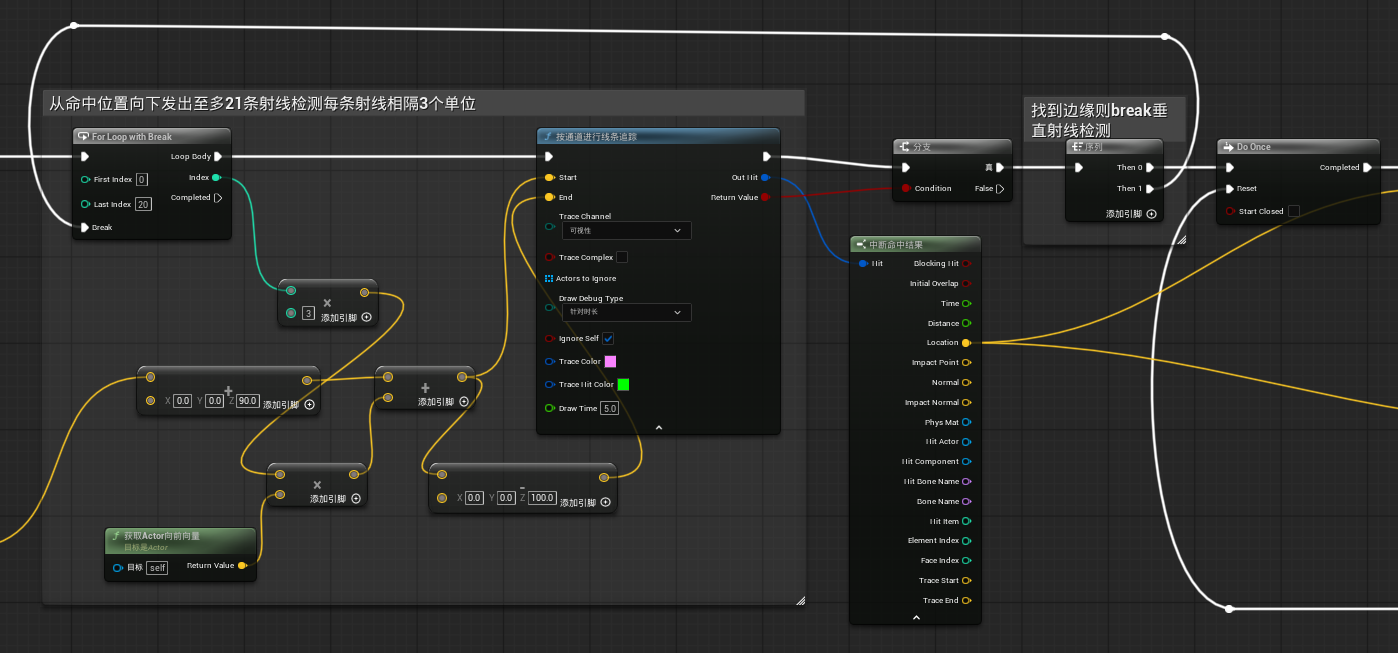
\includegraphics[width=1.0\textwidth]{抓边攀爬2.png}
\caption{抓边攀爬}
\end{figure}

\begin{figure}[h]
\centering
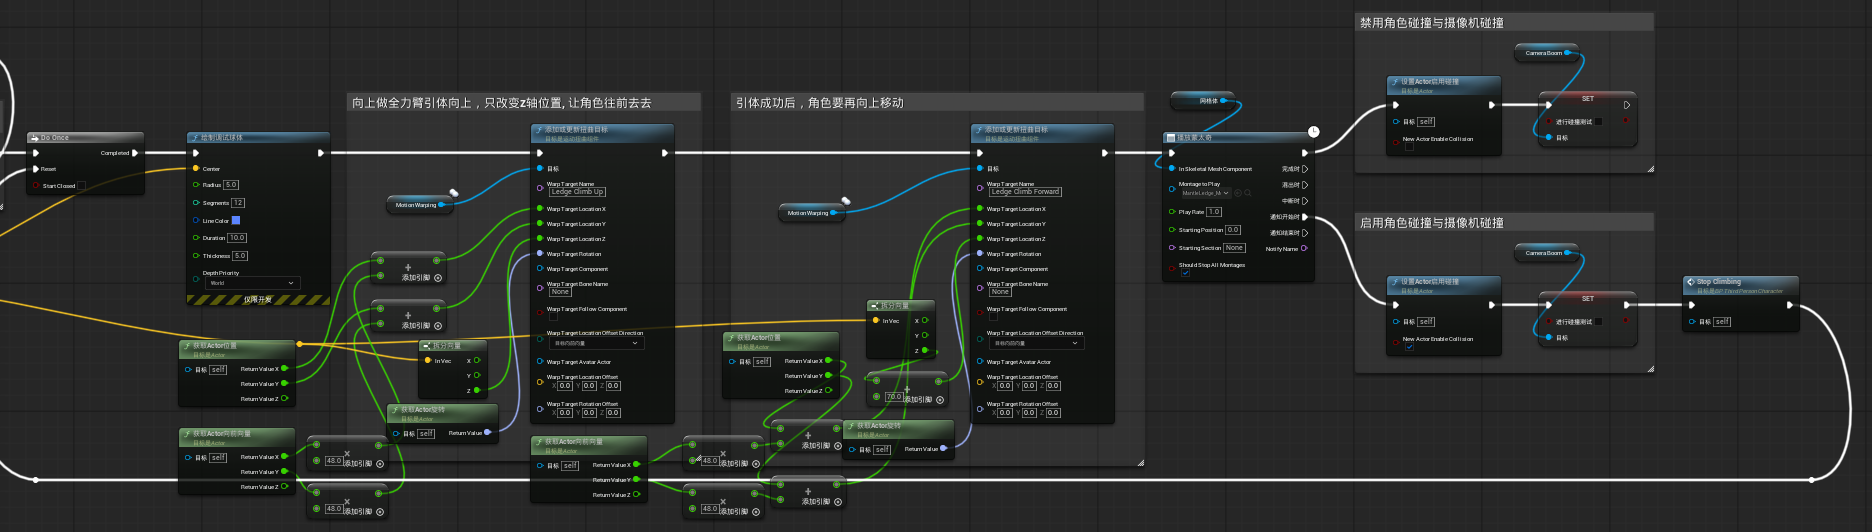
\includegraphics[width=1.0\textwidth]{抓边攀爬3.png}
\caption{抓边攀爬}
\end{figure}





%--------------------------------------------------------------------------AI
\chapter{AI系统} 

\section{AI行为树巡逻}

\begin{itemize}
    \item 新建AI文件夹
    \item 新建“人工智能”“黑板”BD\_AI，作为AI通用的黑板模板；新建“人工智能”“行为树”BT\_AI；确保将黑板资产连接到行为树
    \item 新建“蓝图类”“AIController”，作为AI类通用的控制器。事件开始运行时，运行行为树
    \item 复制BP\_Dummy为BP\_AI，“细节”中搜索AI，修改AI控制器类，更改“自动控制AI”->已放置在场景中或已生成
    \item 在行为树中新建序列巡逻，新建文件夹task，在里面添加任务BP\_Task\_PatrolRandomPoints（巡逻随机点）（F5.36）
    \item 在关卡中快速添加“体积”“寻路网格体体积边界”，设置包裹全地图，按下p键可以看到所有可能的路径
    \item AI此时可以移动，但没有动画。旋转太生硬-> 关闭“细节”“使用控制器旋转Yaw”，开启“角色移动”“把旋转朝向运动”，并创建AI自己的动画蓝图。给AI应用该ABP

\end{itemize}

\begin{warning}
修复装备UI界面可以攻击的bug -> 引用并修改攻击系统中的canAttack变量
\end{warning}

\begin{warning}
修复装备UI槽在选取装备项后没有自动关闭的问题 ->  按了SlotItem后，设置装备列表不可见
\end{warning}


\begin{warning}
修复装备UI槽在关闭重新打开后值被取消的bug -> 每个UI本质上是一个Actor，当关闭装备栏再打开时，它已经是另一个实例了 -> 将需要保存的信息传入角色中（暂不修复）
\end{warning}

\begin{tip}
行为树的执行顺序：自上而下，自左而右
\end{tip}

\begin{figure}[h]
\centering
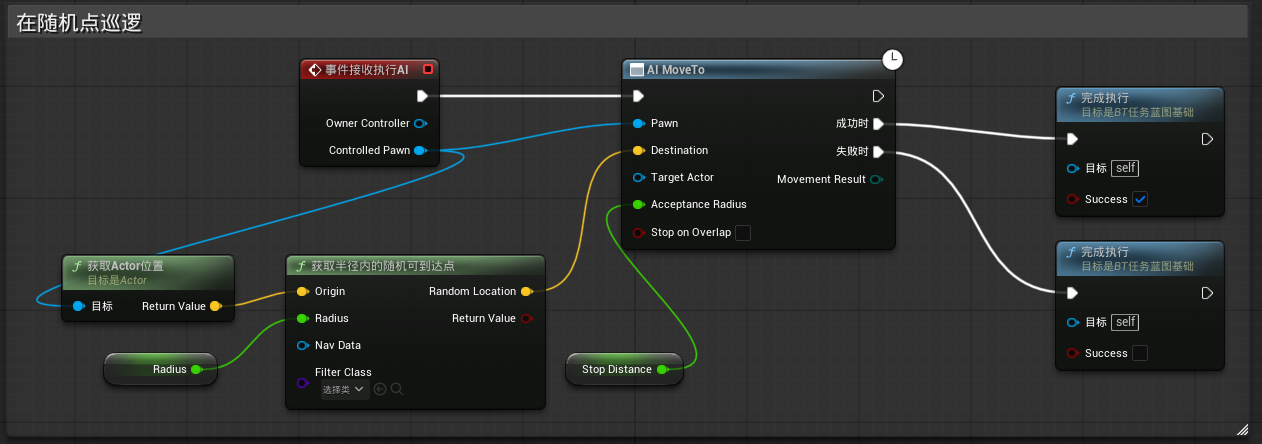
\includegraphics[width=1.0\textwidth]{AI随机巡逻任务.png}
\caption{AI随机巡逻任务}
\end{figure}


%---------------------------------------------新章节
\section{AI侦测与追击}

视觉：
\begin{itemize}
    \item 给AI控制器添加AI Perception组件，给“感官配置”增加视觉感官，启用全部按归属检测。给控制器添加获取刺激来源的逻辑（F5.37）
    \item 行为树增加追逐目标序列，并且拖到巡逻左边。右键添加装饰器“黑板”（相当于判定条件）
    \item 给玩家角色添加AI感知刺激源组件，勾选自动注册源，添加“视觉”
    \item 修改默认游戏配置，取消自动注册角色为刺激源
\end{itemize}

听觉：
\begin{itemize}
    \item 给AI感知组件“感官配置”增加"AI监听配置"
    \item 将F5.37的事件改为一个函数Sight Detection，为听觉添加类似的函数（黑板中增加Investigation Location位置变量）（F5.43）
    \item 状态树中新建序列Investigation Sequence，当没看到目标时，如果听到声音则去声音发出的调查点调查，否则在随机点巡逻（F5.44）
    \item 给主角新增一个调试键，调用“报告噪音事件”
    \item 给AI添加调查图标-> 制作一个widget -> BP\_AI添加这个组件，事件中写一个逻辑（F5.45）启用这个组件
\end{itemize}




\begin{figure}[h]
\centering
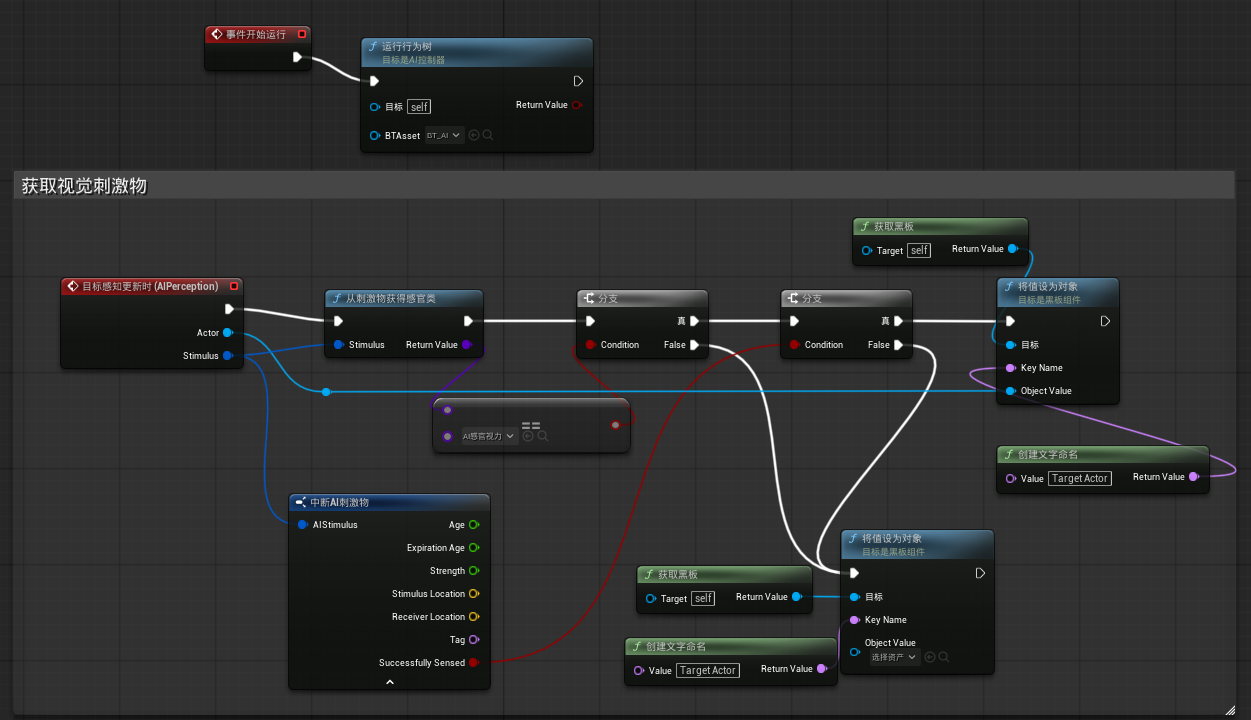
\includegraphics[width=1.0\textwidth]{获取视觉刺激物.png}
\caption{获取视觉刺激物}
\end{figure}

\begin{tip}
视角对准想看的ai，按下'键可以进入AI感知调试
\end{tip}

\begin{warning}
UE中默认所有pawn和character自带刺激源 -> 去Config -> DefaultGame.ini设置 [/Script/Engine.GameModeBase] DefaultPawnClass=None
\end{warning}

%---------------------------------------------新章节
\section{AI近战攻击}

\begin{itemize}
    \item 黑板中新建变量inAttackRange,新建Services服务文件夹，在行为树中新建服务获取与目标之间距离，给追击目标序列添加服务
    \item 新建任务“攻击目标”（F5.39，延迟使得动画可以播放完毕，不会一直在动画的第一帧），放在追逐目标右边，并新建装饰器添加条件。使用并行结构保证两个任务都会做，且完成模式改为延迟（F5.40）
    \item 给BP\_AI添加攻击任务中用到的接口，并双击左边“接口”中Attack函数实现(F5.41)。
    \item 目前ai的攻击逻辑只是播放一个动画，我们首先将玩家角色中的连击动画系统复制到BP\_AI中,修改其中的自定义事件并创建变量。然后为连招中的通知事件添加ai处理逻辑（F5.42）。接着为AI创造类似的追踪碰撞逻辑。最后，伤害只会施加给可受伤的敌人，玩家需要也有这个标签
    \item AI目前和我们碰撞会将角色弹飞 ->更改AI的碰撞预设为无碰撞，角色死亡时布娃娃逻辑中更改碰撞类型为“物理形体”。并给ai加上模型剑
\end{itemize}

\begin{figure}[h]
\centering
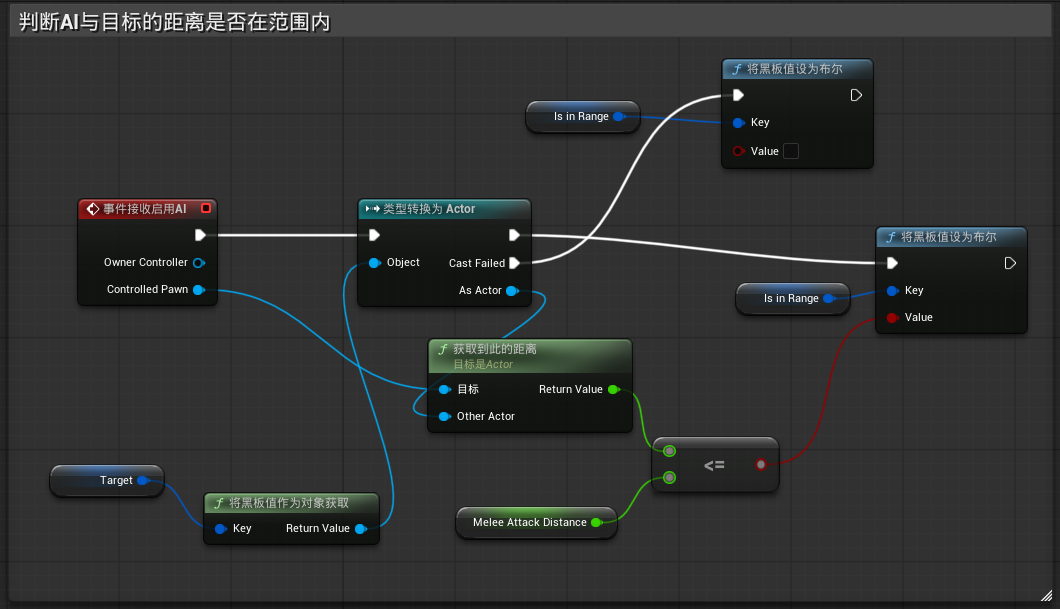
\includegraphics[width=1.0\textwidth]{判断AI与目标的距离.png}
\caption{判断AI与目标的距离服务}
\end{figure}

\begin{figure}[h]
\centering
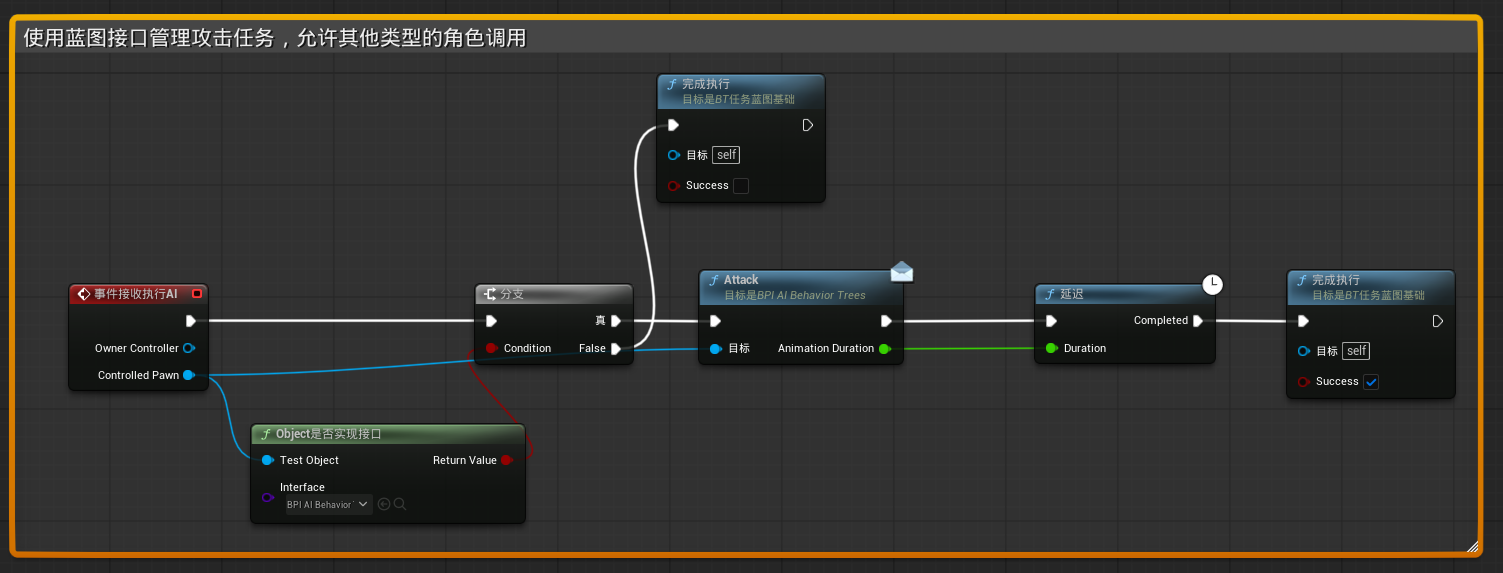
\includegraphics[width=1.0\textwidth]{攻击任务.png}
\caption{攻击目标}
\end{figure}

\begin{figure}[h]
\centering
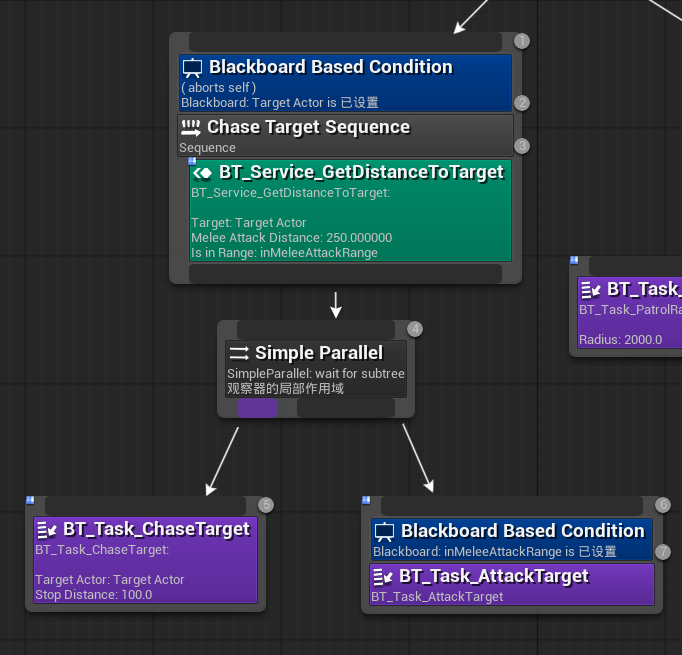
\includegraphics[width=1.0\textwidth]{添加攻击逻辑的行为树.png}
\caption{添加攻击逻辑的行为树}
\end{figure}

\begin{figure}[h]
\centering
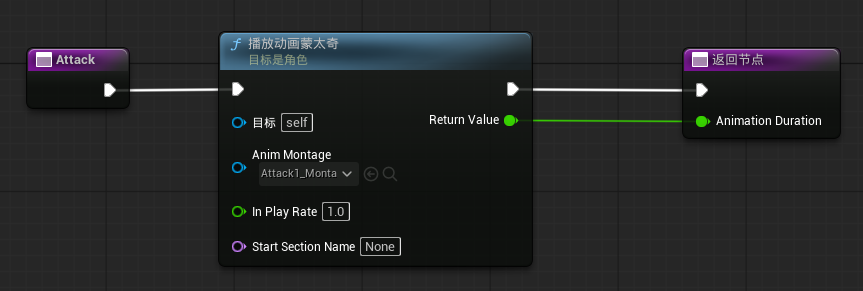
\includegraphics[width=1.0\textwidth]{Attack函数.png}
\caption{Attack函数}
\end{figure}


\begin{figure}[h]
\centering
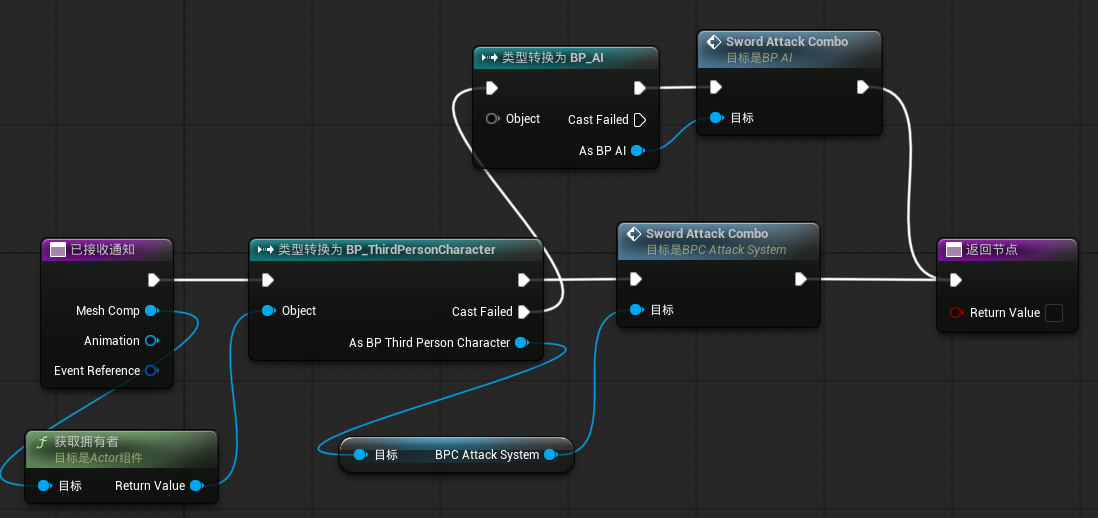
\includegraphics[width=1.0\textwidth]{通知逻辑修改实例.png}
\caption{通知逻辑修改实例}
\end{figure}

\begin{warning}
     F5.38的逻辑中，AI只会在一开始计算与目标距离，导致它进入连击后不会再计算从而一直连击 -> 将开始事件改为Tick AI
\end{warning}


\begin{warning}
     角色的脚一直是平行的 -> ik修复： 启用Control Rig（绑定控制），并在没有下落时启用射线检测 -> 脚可以更大程度的贴合环境
\end{warning}

\begin{warning}
     蹲伏时修改胶囊体变小，但是如果在地形下站起来，则会卡入地形中 -> 增加射线检测，头顶有障碍物不允许站立 （F5.46）
\end{warning}




\begin{figure}[h]
\centering
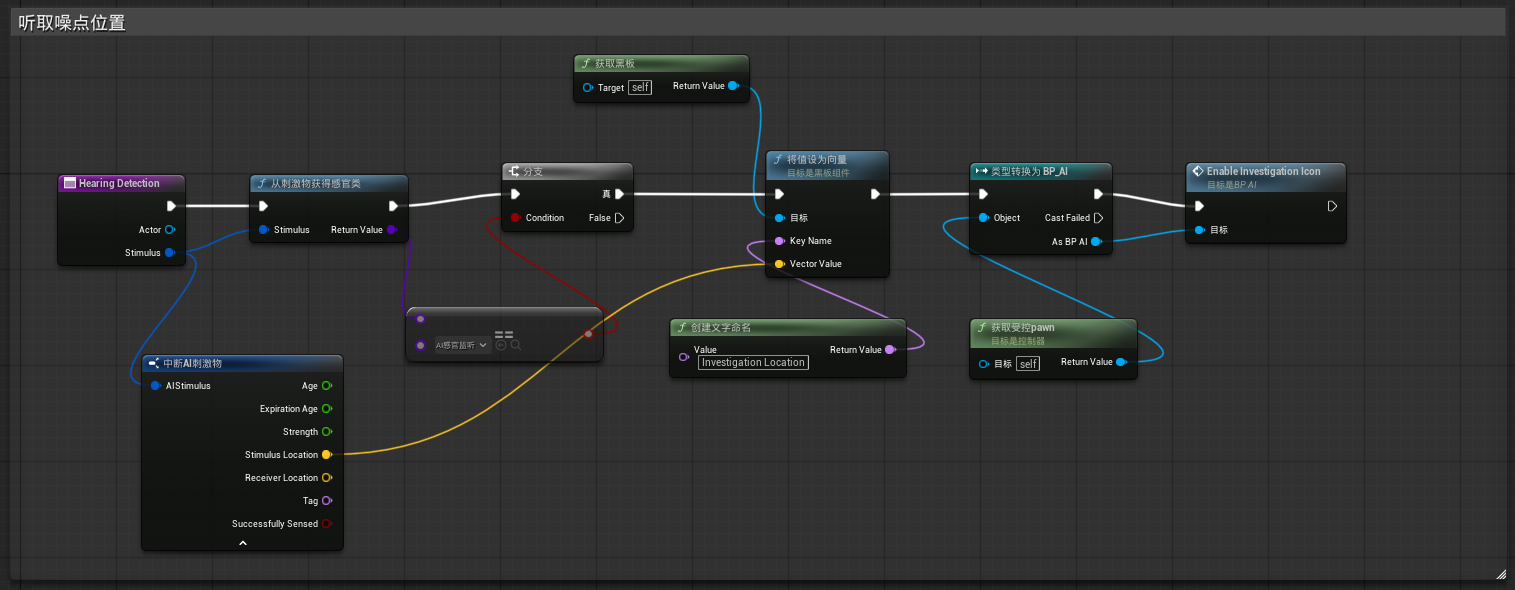
\includegraphics[width=1.0\textwidth]{监听噪点.png}
\caption{监听噪点}
\end{figure}

\begin{figure}[h]
\centering
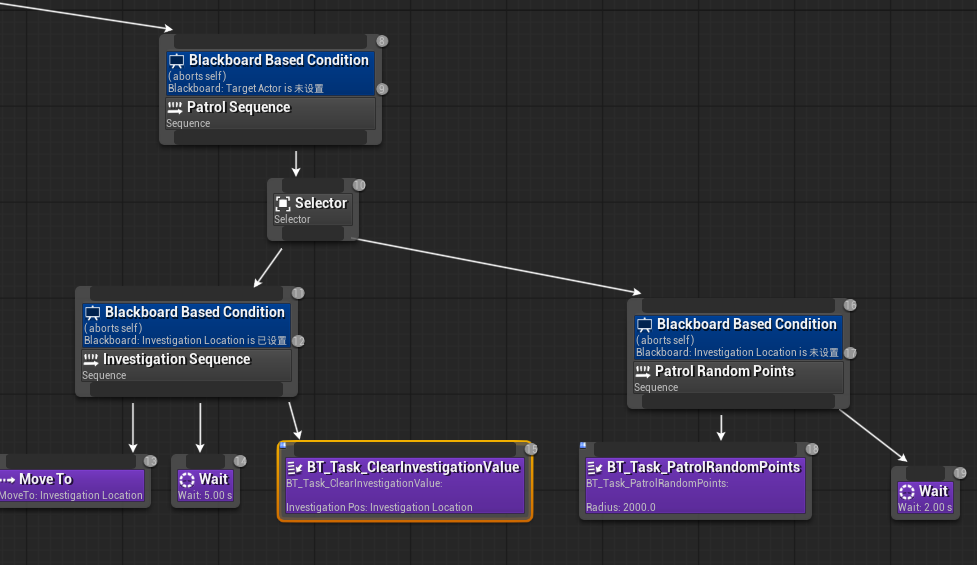
\includegraphics[width=1.0\textwidth]{调查噪点.png}
\caption{调查噪点}
\end{figure}

\begin{figure}[h]
\centering
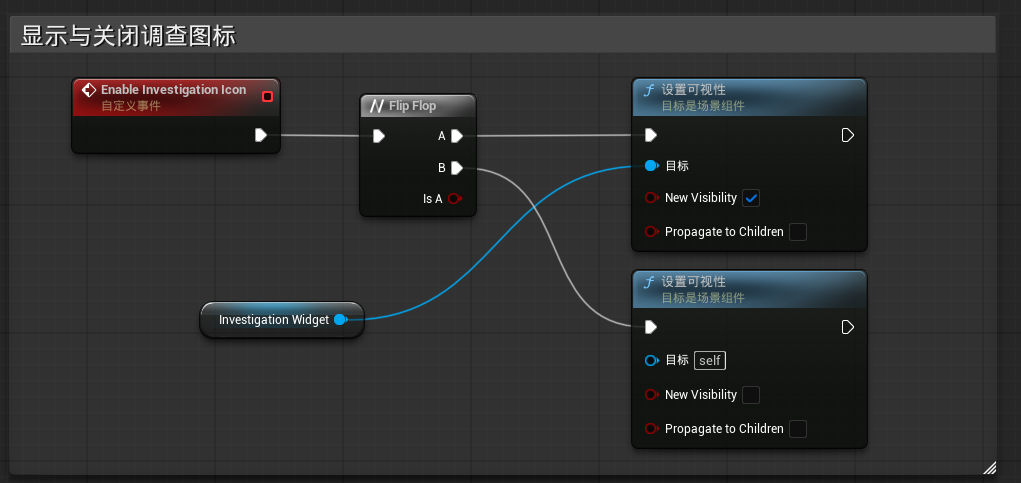
\includegraphics[width=1.0\textwidth]{调查图标.png}
\caption{调查图标}
\end{figure}

\begin{figure}[h]
\centering
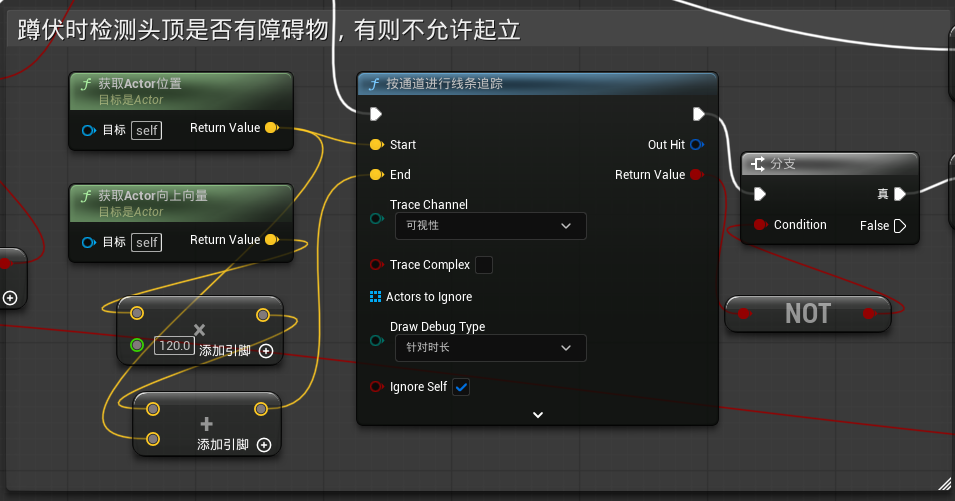
\includegraphics[width=1.0\textwidth]{头顶射线检测.png}
\caption{头顶射线检测}
\end{figure}



%---------------------------------------------新章节
\section{投掷物干扰AI}

允许玩家投掷物品，物品落地后发出噪点，吸引AI前往调查：
\begin{itemize}
    \item 新建文件夹Interact，复制攻击1动画（这个动画本身就像在投掷一个物体）并改名ThrowObject，移除多余的帧，调整播放速率更慢
    \item 新建输入投掷（E），连接蒙太奇，并建立投掷物体通知点，在通知点时刻生成投掷物体（SpawnActor ）（F5.47）
    \item 新建Actor类BP\_ThrowableObject，添加静态网格体组件(石头模型)，弹射物移动组件，给定初速度和最大速度。将模型设为父级，并给模型添加碰撞体，才能发生碰撞
    \item 最后，给投掷物落地应用干扰噪点：添加事件“组件命中时”连接报告噪音。注意需要给投掷物添加AI刺激源，并且设置为听觉刺激（F5.48）

\end{itemize}


\begin{figure}[h]
\centering
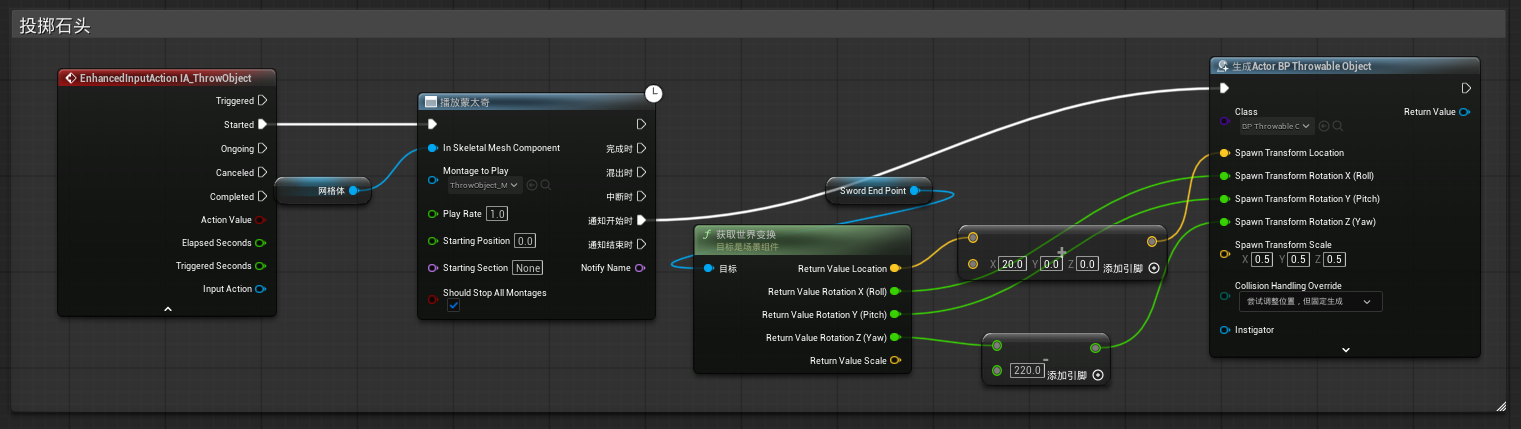
\includegraphics[width=1.0\textwidth]{投掷石头.png}
\caption{投掷石头}
\end{figure}

\begin{figure}[h]
\centering
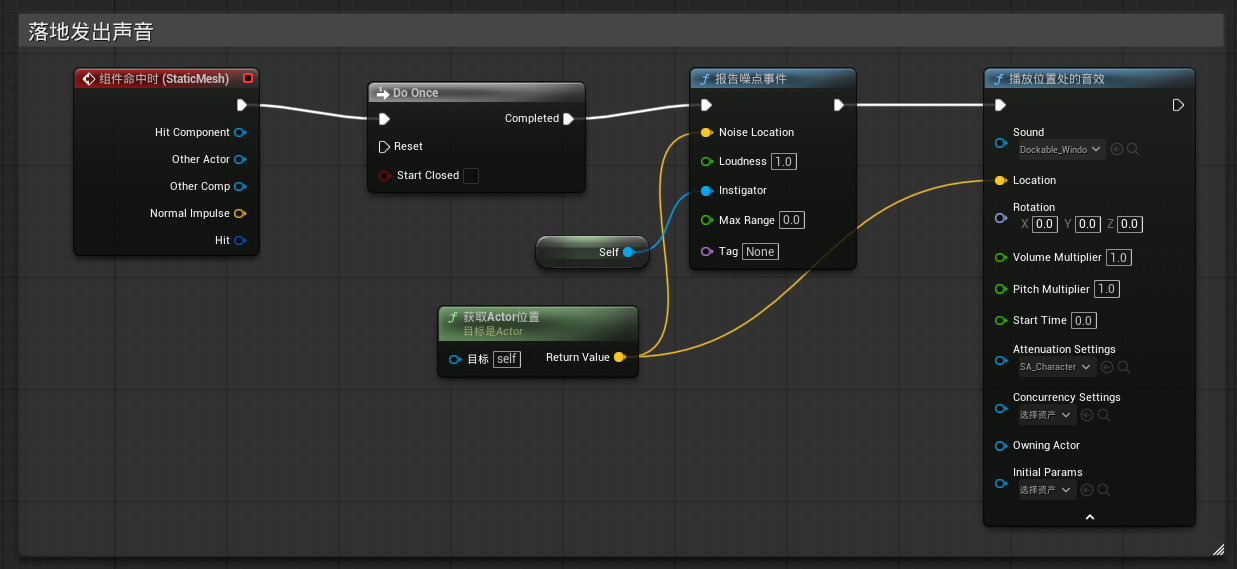
\includegraphics[width=1.0\textwidth]{石头落地.png}
\caption{石头落地}
\end{figure}



%---------------------------------------------新章节
\section{首领AI}
\begin{itemize}
    \item 在BP\_AI上右键，创建子蓝图类BP\_AI\_Boss,放大模型，减慢移动速度。更改ai控制器，行为树（需更改选中的黑板）
    \item 更改Boss攻击动画播放速率，将父类中动画播放速率提升为变量，并公开 -> Boss中可以在类默认值中找到这个变量并且设置
    \item 创建用于显示Boss的UI控件，并在Boss控制器的事件中实现激活逻辑，在父类中调用（F5.49）。并且实时更新来自Boss属性系统的血量值(F5.50)
    
    \item 类似的，我们创造平民AI（只会巡逻），调整速度（角色移动组件）和巡逻范围(行为树中task)。平民没有血条，且不允许被攻击（将父类的damageable标签移除，给需要的子类添加）
    

\end{itemize}

\begin{warning}
    修复生命值系统的报错问题 -> 过去的生命值系统只能检测两类蓝图：character 和 dummy,我们将选择节点改用枚举（F5.51）
\end{warning}

\begin{figure}[h]
\centering
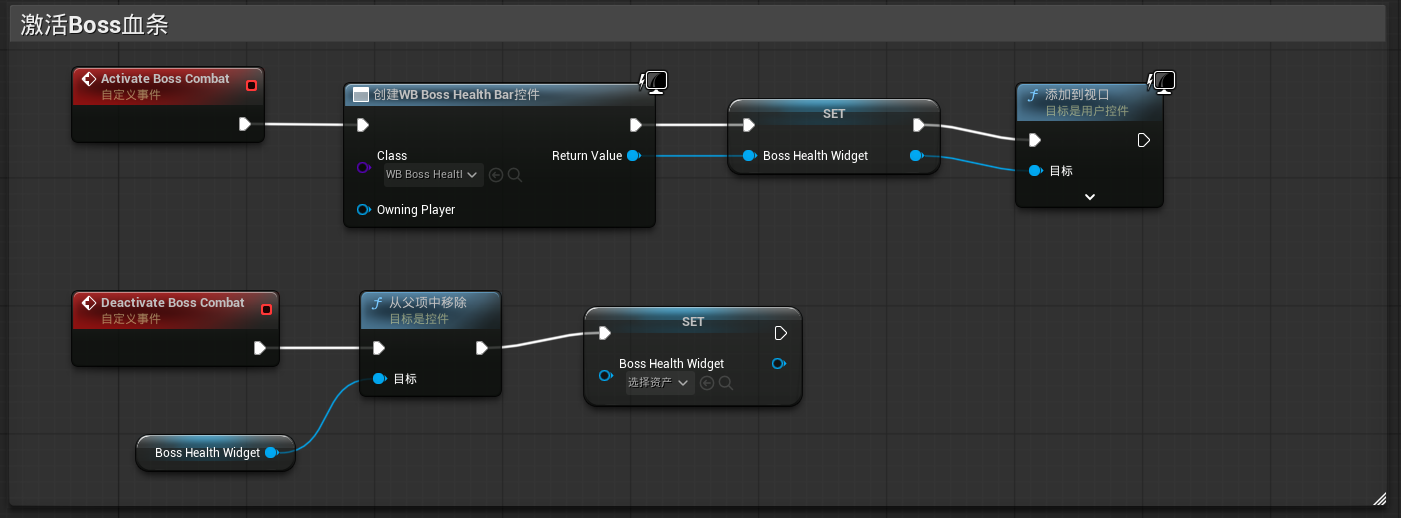
\includegraphics[width=1.0\textwidth]{激活Boss血条.png}
\caption{激活Boss血条}
\end{figure}

\begin{figure}[h]
\centering
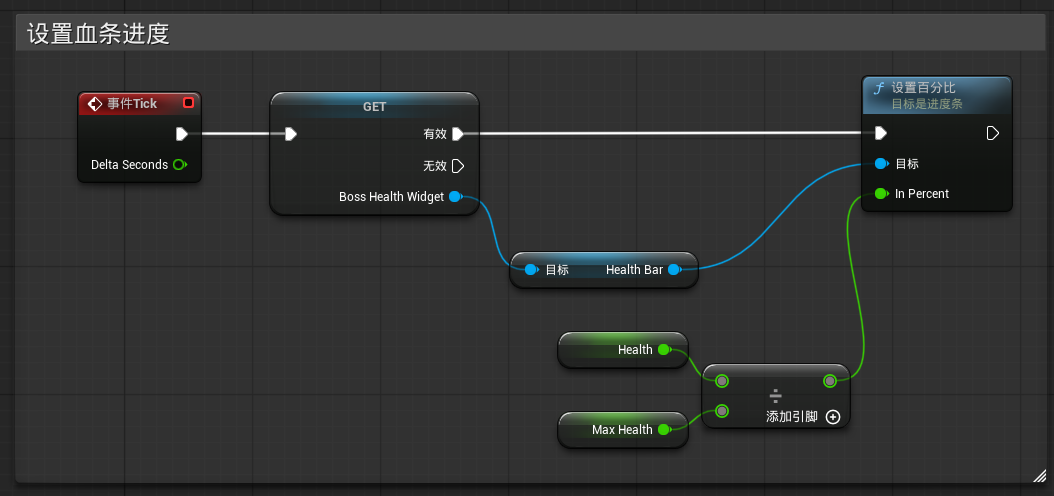
\includegraphics[width=1.0\textwidth]{设置boss血条.png}
\caption{设置Boss血条}
\end{figure}

\begin{figure}[h]
\centering
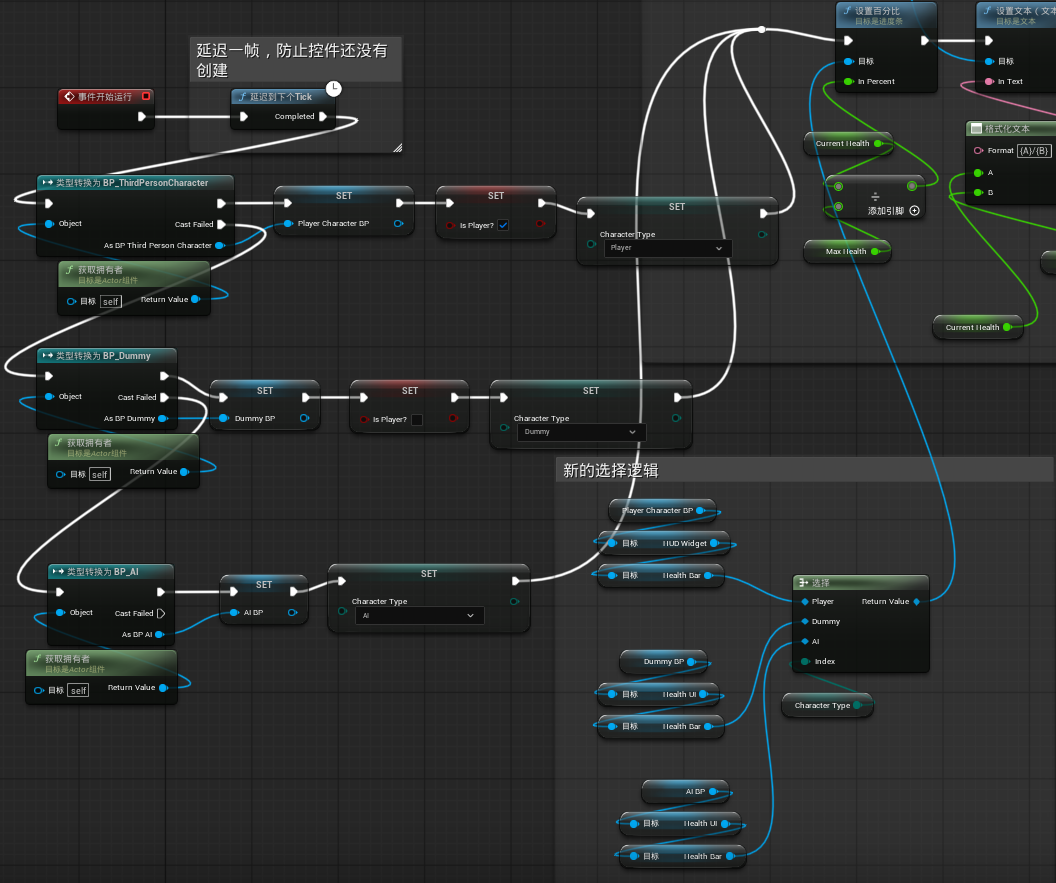
\includegraphics[width=1.0\textwidth]{选择逻辑更新.png}
\caption{选择逻辑更新}
\end{figure}


%--------------------------------------------------------------------------AI
\chapter{弓箭设计系统} 

\section{弓箭动画}

\begin{itemize}
    \item  在动画蓝图中添加三个状态：拉弓，瞄准，射箭
    \item  设置变量isAimingWithBow和hasBow，若角色在瞄准且有弓箭（因为我们有一个取箭的动作），则从locomotion切换到拉弓状态，拉弓动画播放完毕，切换瞄准（转换条件勾选自动序列规则即可）
    \item  如果我们有箭并且停止了用弓瞄准，则射箭
    \item  当装备了弓时，我们希望播放其他的待机动画，所以在idle状态中使用blend执行选择（F7.2）
    \item  给拉弓设计新的输入（鼠标右键）
\end{itemize}


\begin{figure}[h]
\centering
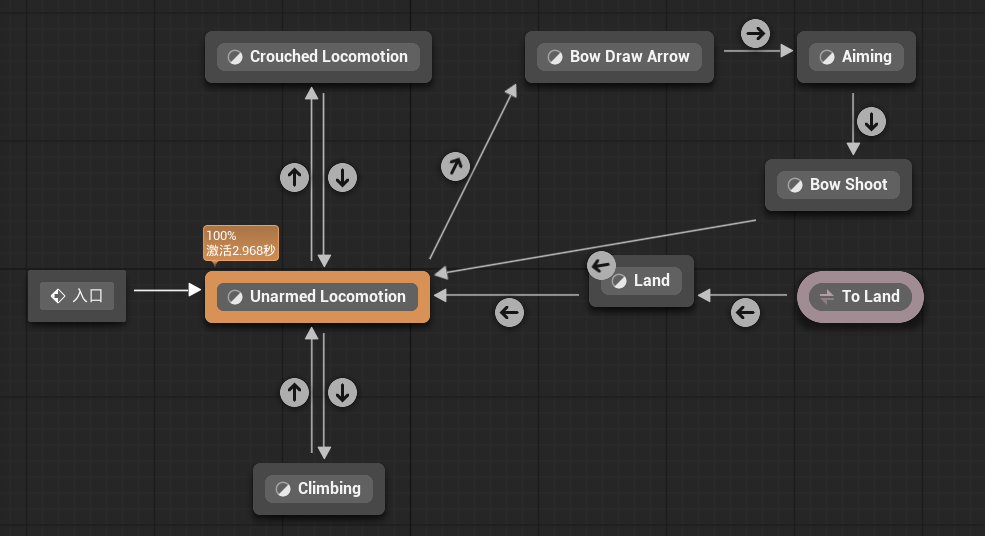
\includegraphics[width=1.0\textwidth]{射箭状态转换图.png}
\caption{射箭状态转换图}
\end{figure}

\begin{figure}[h]
\centering
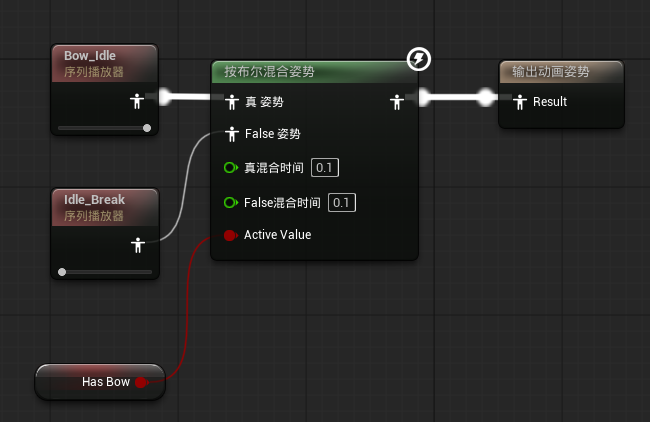
\includegraphics[width=1.0\textwidth]{选择待机动画.png}
\caption{选择待机动画}
\end{figure}

\section{瞄准偏移}

\begin{itemize}
    \item  在Bow文件夹中新建文件夹AO\_Aiming,基于Bow\_Aiming动画，创建几个副本
    \item  以向前瞄准为例，选中第一帧，删除其余的所有帧，启用附加动画“网格体空间”，选择Bow\_Aiming。向上看和向下瞄准同样操作，不过需要额外调整骨骼树中spine03的旋转角（添加关键帧）
    \item  将这三个瞄准统一放在一个“瞄准偏移”中，水平上设置变量pitch，管理俯仰角 
    \item  首先需要在主状态机输出姿势的末尾，依据alpha值启用瞄准偏移动画（F7.3）
    \item  接着需要在有弓箭时才启用瞄准偏移（设置alpha为1），同时设置动画需要的俯仰角变量（F7.4）
 
\end{itemize}

\begin{figure}[h]
\centering
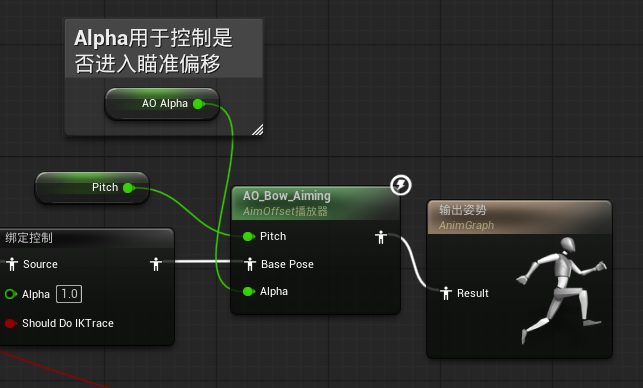
\includegraphics[width=1.0\textwidth]{动画中调用瞄准偏移.png}
\caption{动画中调用瞄准偏移}
\end{figure}

\begin{figure}[h]
\centering
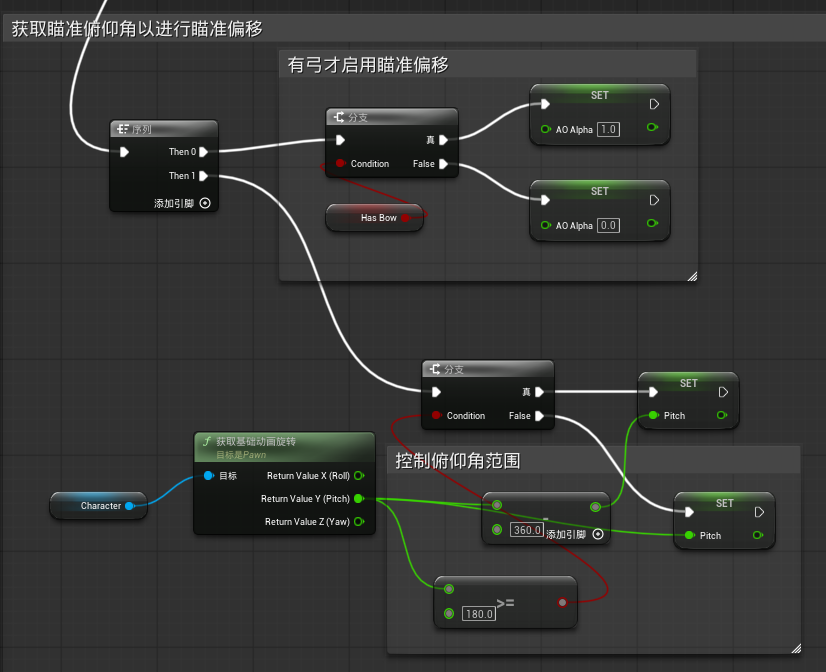
\includegraphics[width=1.0\textwidth]{设置瞄准偏移俯仰角.png}
\caption{设置瞄准偏移俯仰角}
\end{figure}

\section{手持弓箭}
\begin{itemize}
    \item  给骨骼手部创立拿弓的插槽，这里可以使用预览动画，原来的动画可以复制一份重新绑定骨骼
    \item  创立一个静态网格体绑定手部的持弓插槽，给其设置弓箭网格体。当装备弓箭时，令背部的弓不可见，同时，令手部的弓可见（F7.5）
    \item  令瞄准时视角锁定，始终指向玩家的正前方（F7.6）
    \item  创建新的Actor类BP\_Arrow，参考之前做的可投掷物对象（石头吸引ai），添加静态网格体组件（箭），并将其设置为根。
    \item  添加发射物移动组件，设置初速度和最大速度，禁用反弹。
    \item  在射击时生成箭：新建一个AnimNotify通知（F7.7），在动画射击时发出该通知。
    \item  在角色蓝图中手中弓下创建一个箭头，用于标记生成的箭的位置和方向
    \item  在角色时间中建立“射箭”事件（F7.8），收到通知后调用该事件，在恰当的位置生成actor箭

\end{itemize}

\begin{figure}[h]
\centering
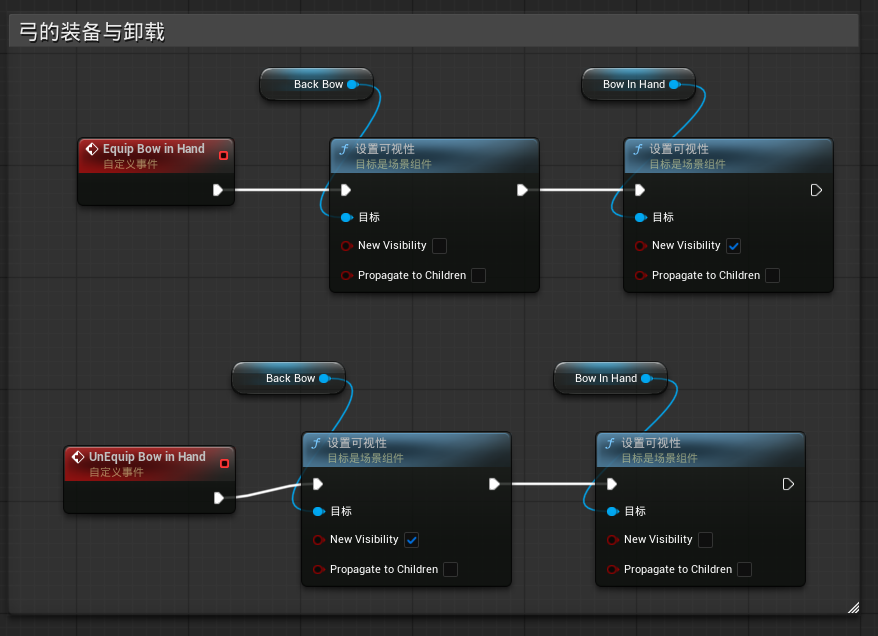
\includegraphics[width=1.0\textwidth]{弓的装备和卸载.png}
\caption{弓的装备和卸载}
\end{figure}

\begin{figure}[h]
\centering
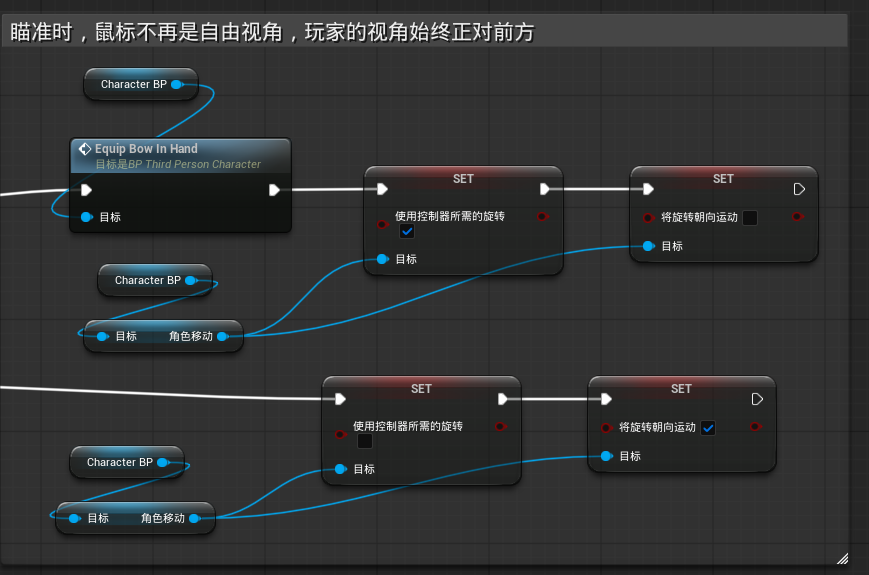
\includegraphics[width=1.0\textwidth]{锁定瞄准视角.png}
\caption{锁定瞄准视角}
\end{figure}

\begin{figure}[h]
\centering
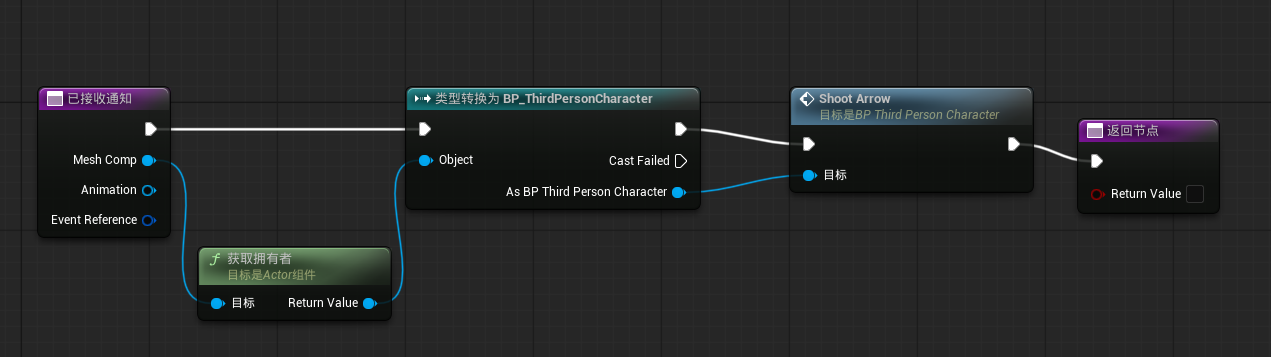
\includegraphics[width=1.0\textwidth]{射箭通知.png}
\caption{射箭通知}
\end{figure}

\begin{figure}[h]
\centering
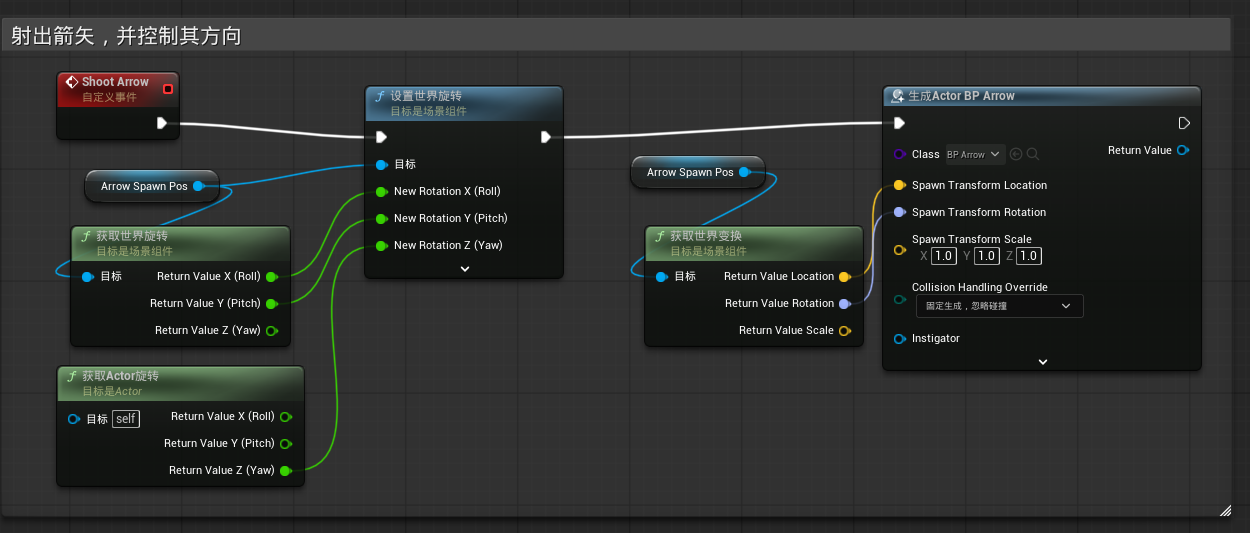
\includegraphics[width=1.0\textwidth]{射箭.png}
\caption{射箭}
\end{figure}

\section{瞄准移动}
\begin{itemize}
    \item  导入箭模型后，初始箭的方向并不指向x轴正方向，导致生成箭时箭的方向不对 -> 在场景中拖入箭模型的静态网格体，使用建模模式编辑轴枢点，使其指向x轴正方向
    \item  在之前的逻辑中，一旦我们进入瞄准状态，那么始终播放瞄准动画，因此即使角色移动，也是瞄准动画在平移 -> 进入瞄准状态机，令瞄准和身体下半身混合。
    \item  在“每个骨骼的分层混合”中，基础动画选择locomotion，混合动画选择瞄准，并在右侧的层设置中，添加索引骨骼"spine\_01",设置“混合深度”为8，并勾选“网格体空间旋转混合”（F7.9）
    \item  在拉弓时，我们需要拉满弓才会切换动画，因此此时奔跑也会平移 -> 使用相同的方法分层混合。射击完毕后同理。
\end{itemize}

\begin{figure}[h]
\centering
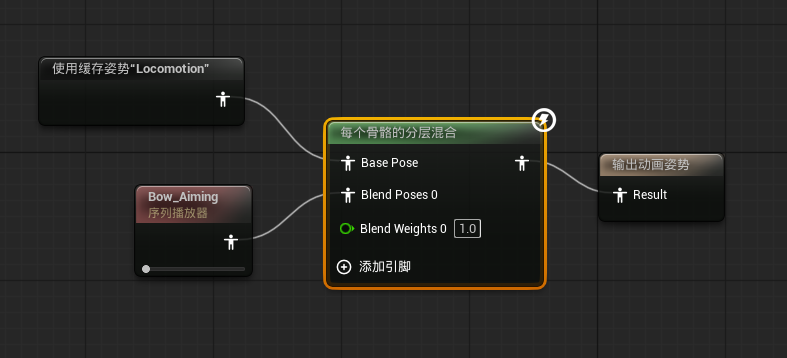
\includegraphics[width=1.0\textwidth]{混合瞄准与奔跑.png}
\caption{混合瞄准与奔跑}
\end{figure}



\section{弓箭伤害}
\begin{itemize}
    \item  新建射击准星UI，在玩家攻击系统中，开始瞄准后设置该UI可见。并且稍微移动一下摄像机角度，给一个摄像机臂的偏移（时间轴）（F7.10）
    \item  给箭的蓝图添加当组件开始重叠时(F7.11)，并且在刚开始的一会，禁用箭矢的碰撞，以防玩家移动撞到箭
    \item  调整箭的生成点与准星对齐，将箭矢生成位置由弓的子对象改为摄像机的子对象，并取消之前的旋转箭头朝向与视角对齐逻辑
\end{itemize}


\begin{figure}[h]
\centering
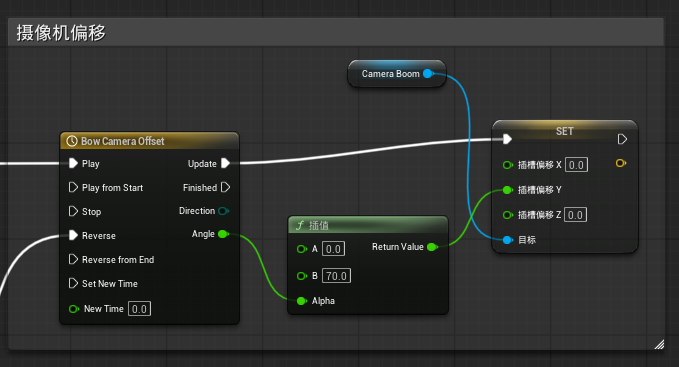
\includegraphics[width=1.0\textwidth]{摄像机偏移.png}
\caption{摄像机偏移}
\end{figure}

\begin{figure}[h]
\centering
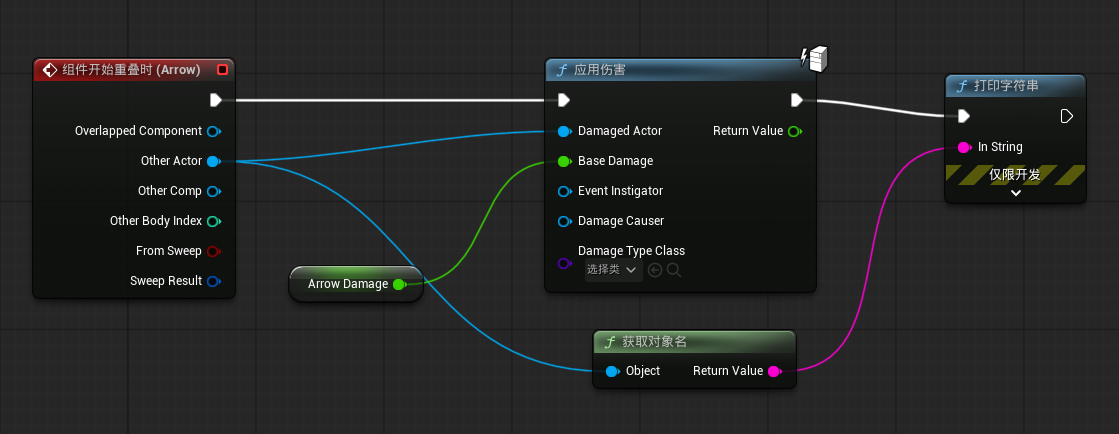
\includegraphics[width=1.0\textwidth]{箭伤.png}
\caption{箭伤}
\end{figure}


%---------------------------------------------新章节
\chapter{开放世界} 

\begin{itemize}
    \item 文件 -> 新建关卡 -> 基础模板，将关卡保存在新建文件夹Levels下，命名为desert
    \item 设置游戏模式，删除原来的地面，创建新地形，设置玩家起始位置
    \item 使用landmass插件创建地形，进入“地形”模式，选择“蓝图”，蓝图笔刷 CustomBrush MaterialOnly，并更改笔刷材质（噪声）
    \item 在Quixel Bridge中找到Bright Desert Sand，下载后拖入LandScape的地形材质
    \item 调整光照并启用体积雾，调整雾密度和消光范围
    \item 添加视觉效果，后期处理体积，重置位置并勾选无限范围（未绑定），调整曝光，全局饱和度和对比度
    \item 添加Water插件，在“快速添加”“所有类”中查找water body lake，将碰撞预设改为overlapalldynamic
    \item 添加棕榈树与岩石资源，在“选择模式”中选择植被，拖入植物资源。调整笔刷尺寸与绘制密度。可以为素材添加Nanite

\end{itemize}

\begin{tip}
按住ctrl + l，移动鼠标，调整光照

\end{tip}


\section{游泳}
\begin{itemize}
    \item 在第三人称角色中添加游泳逻辑（F8.1）
    \item 将湖泊转化为蓝图，并触发玩家游泳逻辑(F8.2)，注意需要给玩家打上标签
    \item 导入游泳动画，依据速度创立混合空间。连接主状态机中的locomotion。游泳时需要禁用ik
    \item 设置水体的碰撞高度偏移为负数，以免刚一碰到水，玩家就开始游泳了

\end{itemize}

\begin{figure}[h]
\centering
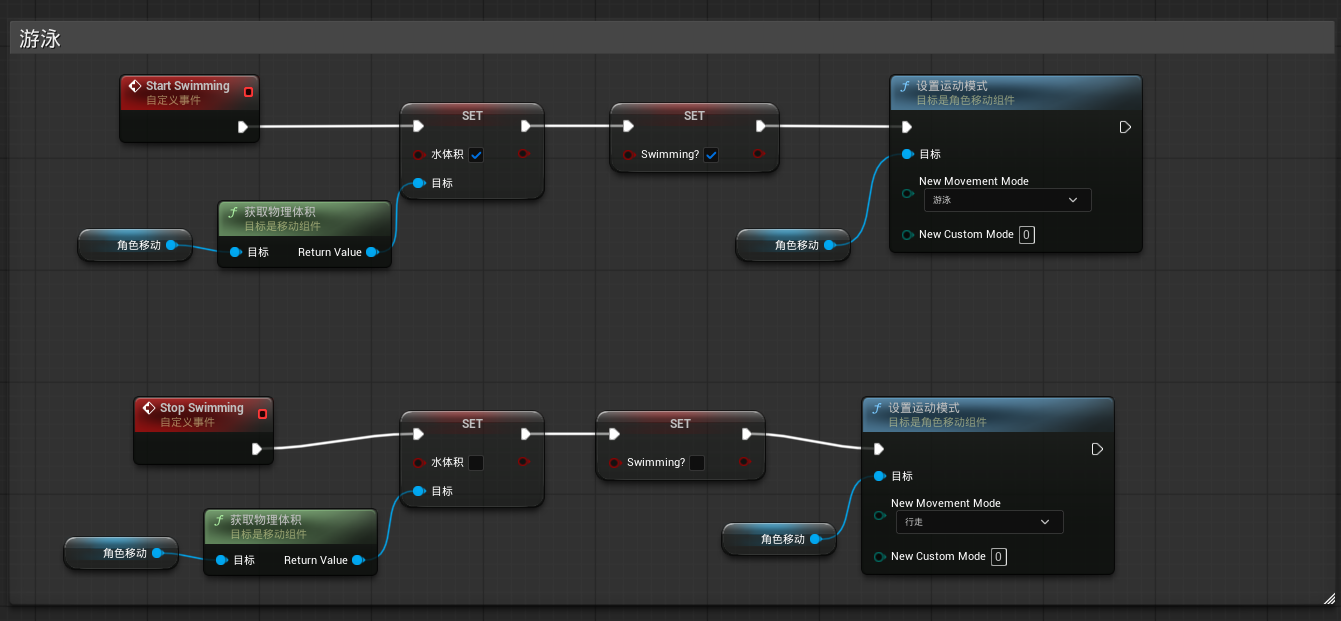
\includegraphics[width=1.0\textwidth]{游泳.png}
\caption{游泳}
\end{figure}


\begin{figure}[h]
\centering
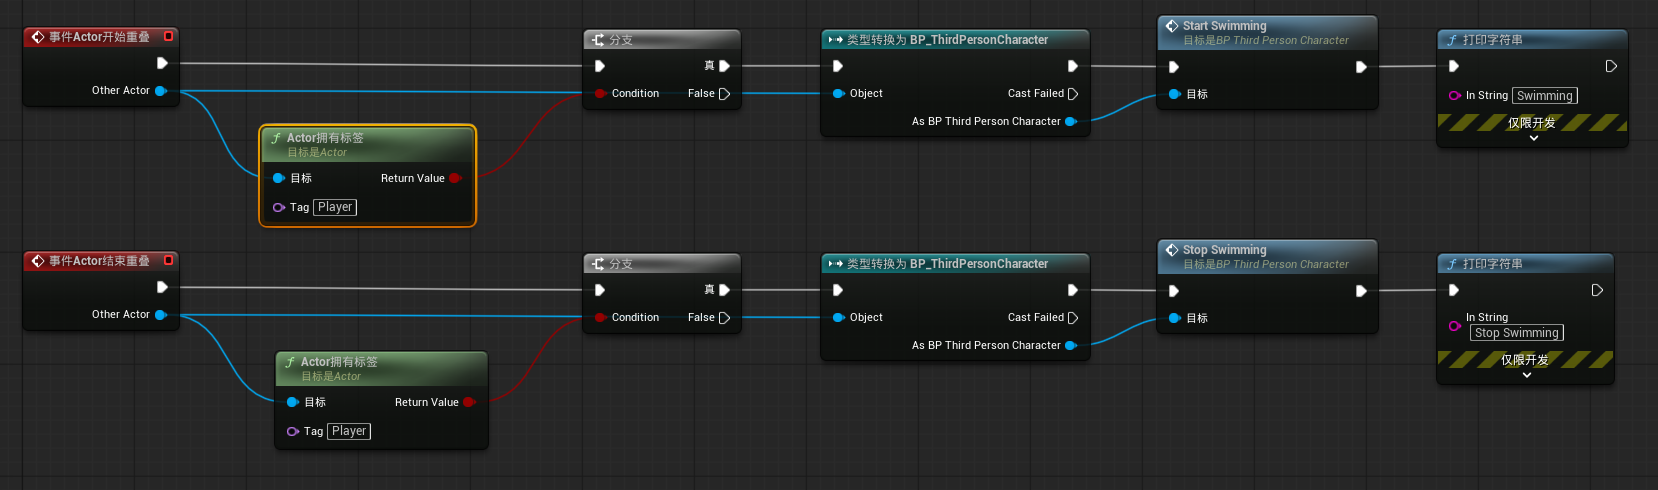
\includegraphics[width=1.0\textwidth]{湖泊蓝图.png}
\caption{湖泊蓝图}
\end{figure}

%--------------------------------------------新章节

\section{动物人工智能}
\begin{itemize}
    \item 使用非洲动物包，设立动物角色蓝图。注意设置移动速度，以及“使旋转朝向运动”，并禁用“使用旋转器控制yaw”，并完成游荡逻辑（不使用行为树与黑板控制，在事件中完成 F8.3）
    \item 以河马为例，创建动画蓝图。生成从待机到行走的混合空间（选择相应骨骼）,连接到动画输出。从父类创建子类，可以实现各个动物。
    \item 给动物父类实现攻击系统：添加Pawn Sensing组件（比AI perception更简单且直接），在“看见pawn”中实现逻辑。需要给动物攻击动画的蒙太奇添加蒙太奇通知，从而开始攻击检测。（F8.4）注意攻击需要控制频率，我们通过is Attacking变量保证完成动画播放再攻击下一次
    \item 在蓝图中编写在某处播放音效，在角色动画中添加通知“play sound”，实现动物走路脚步
  

\end{itemize}

\begin{figure}[h]
\centering
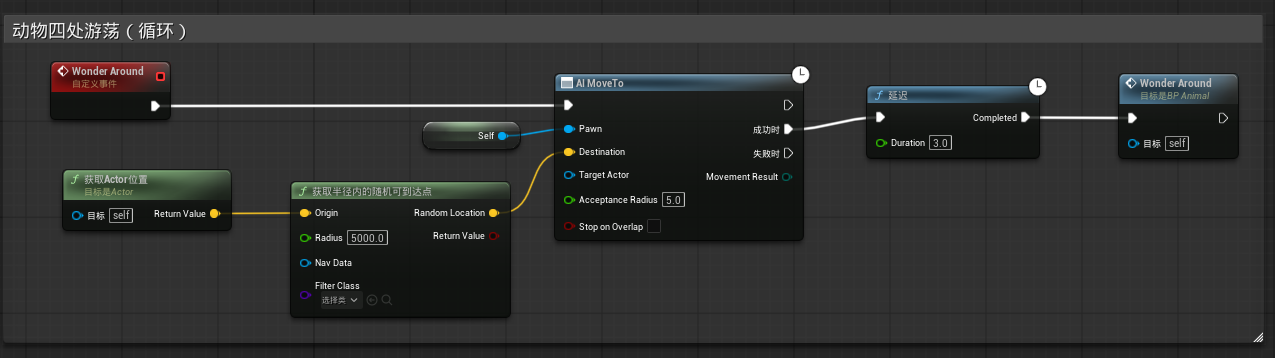
\includegraphics[width=1.0\textwidth]{动物游荡.png}
\caption{动物游荡}
\end{figure}

\begin{figure}[h]
\centering
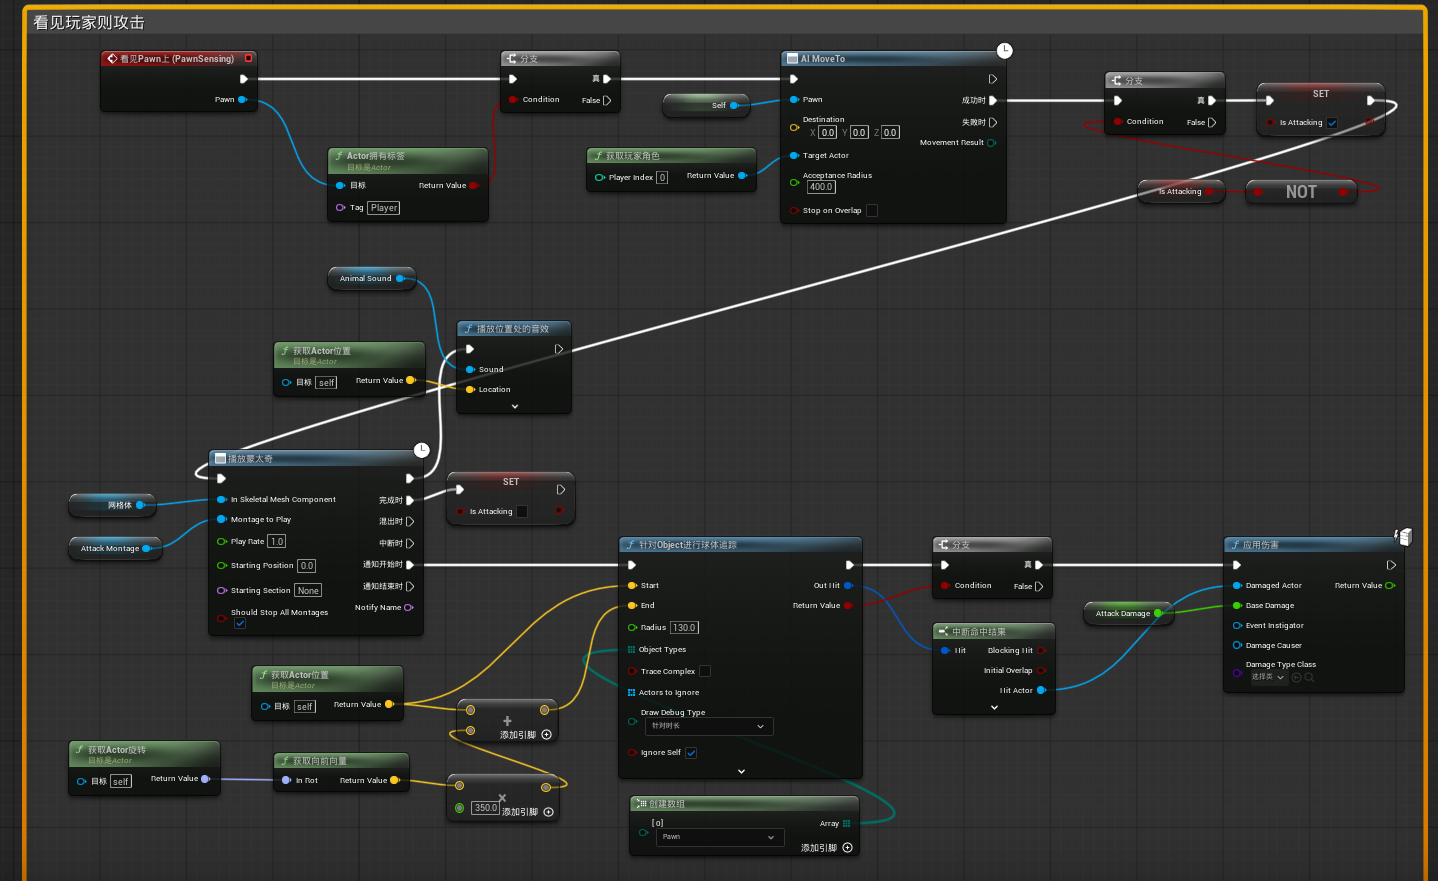
\includegraphics[width=1.0\textwidth]{动物攻击.png}
\caption{动物攻击}
\end{figure}

%--------------------------------------------新章节
\section{玩家受击反馈}

\begin{itemize}
    \item 玩家收到攻击时，除了减少血量，还需要有受击反馈，并设置ui提醒
    \item 1.播放受击音效，对原始音效创建MetaSound应用随机扰动与音效衰减，并创建Sound Cue实现随机播放
    \item 2.播放受击蒙太奇（随机数组取值），并应用一个力弹射角色
    \item 3.在角色HUD中添加一个新图像组件，设置为红色，默认alpha为0。为该图像创建一个动画，以alpha值添加几个关键帧 (F8.5)


\end{itemize}

\begin{figure}[h]
\centering
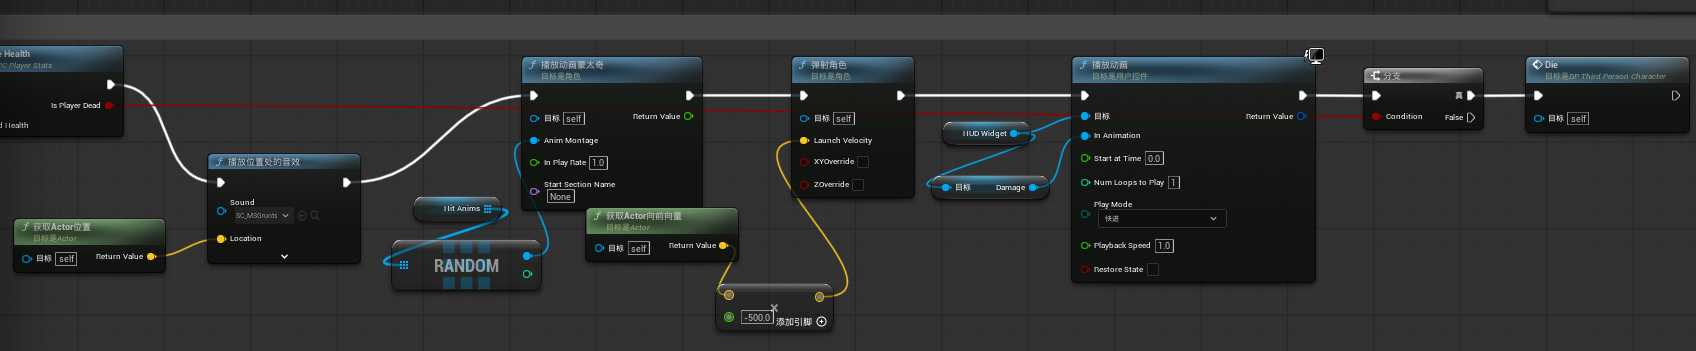
\includegraphics[width=1.0\textwidth]{应用伤害.png}
\caption{应用伤害}
\end{figure}



%---------------------------------------------新章节
\chapter{自我设计}

\section{角色死亡动画}

\begin{itemize}
    \item 目前给角色死亡加了一个动画组，但是这些动画会让角色产生长位移。而角色位移过后，播放完蒙太奇，会率先回到abp中的idle状态，因此会飞回原地
    -> 蒙太奇设置了混出时间，导致在动画的末尾和ABP中的状态混合，设置混出时间为0即可。播放完成后立即设置模拟物理。

    \item 允许根据攻击方向来播放死亡动画：向前和向后（使用攻击者与受击者的前向向量的点积计算）。如果点积大于0,则玩家从背面攻击，角色向前飞

    \item 增加死亡变淡消失的效果。需要在角色材质中“不透明蒙版”连接"DitherTemporalAA"，将Alpha值设为参数。再在函数中调用时间轴将Alpha值从1调整到0（F9.1）

\end{itemize}

\begin{figure}[h]
\centering
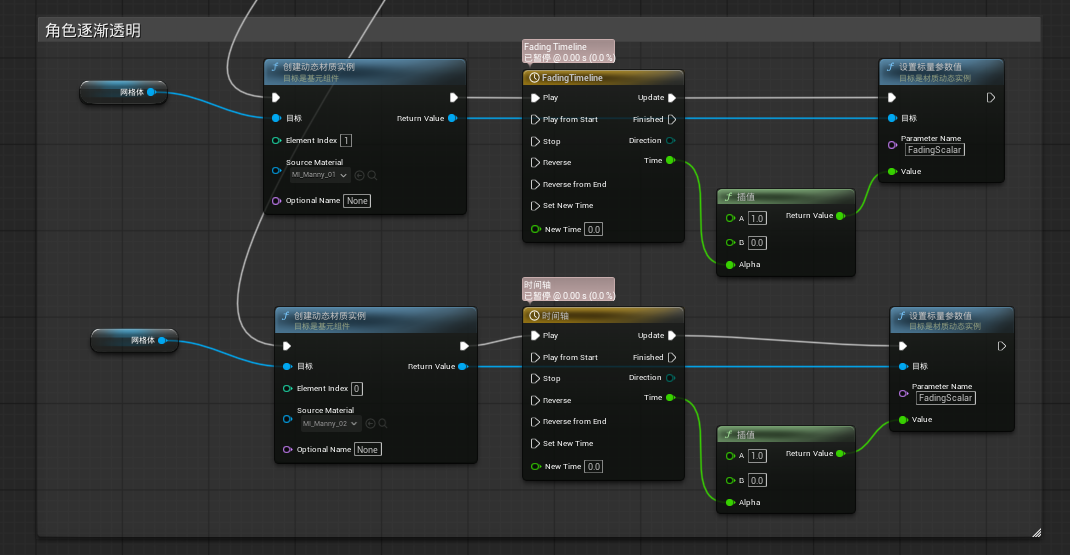
\includegraphics[width=1.0\textwidth]{角色透明.png}
\caption{角色透明}
\end{figure}

%---------------------------------------------新章节

\chapter{游戏概念设计}

1.豪意值，看破值
2.不同的角色间有不同的机制（33号远征队）
3.羁绊系统
4.增强ttk，增加博弈色彩，但不要过长造成了冗余



重大失误：对整个动画文件夹重命名，导致游戏文件崩坏 -> 从git中强行合并到上次提交的分支


% 豪礼1：175套UE卡通场景合集
% 豪礼2：130套游戏音效合集
% 豪礼3：3583个常用UE人物动作
% 豪礼4：400个UE人物角色合集
% 豪礼5：5套UE精选实战教程及素材
% 豪礼6：230套UE各种特效素材
% 豪礼7：1200多棵UE常用树木植物
% 豪礼8：77套UE末日生存场景合集
% 豪礼9：112个UE室内环境场景

% 豪礼1链接：https://pan.baidu.com/s/1kbNqhgJCgBMotc-sXtulaA?pwd=aaaa 提取码: aaaa
% 豪礼2链接：https://pan.baidu.com/s/1r9RSWQ2X1nIrdHqOmPlBYQ?pwd=aaaa 提取码: aaaa
% 豪礼3链接：https://pan.baidu.com/s/1uIUrXbgb5PSPa2lP0uHBKA?pwd=aaaa 提取码: aaaa
% 豪礼4链接：https://pan.baidu.com/s/1Lp0_5ZzvTOPB7WXpP7l1-A?pwd=aaaa 提取码: aaaa
% 豪礼5链接：https://pan.baidu.com/s/17HBec4BYqHKv63F7T95bQA?pwd=aaaa 提取码: aaaa
% 豪礼6链接：https://pan.baidu.com/s/1b6PzCWuZfKw8oAYDTbJfqQ?pwd=aaaa 提取码: aaaa
% 豪礼7链接：https://pan.baidu.com/s/19H0ViniBGjGPWLUC1_HImg?pwd=aaaa 提取码: aaaa
% 豪礼8链接：https://pan.baidu.com/s/1aTvsmtOLVIeOQiEVFnq6Sw?pwd=aaaa 提取码: aaaa
% 豪礼9链接：https://pan.baidu.com/s/1vWcjyzqALyH-HcdO5WeVfA?pwd=aaaa 提取码: aaaa





\end{document}